\documentclass{llncs}

\usepackage{xcolor}
\usepackage{enumitem,amsmath,amssymb}
\usepackage{stmaryrd}    % needed for \mapsfrom
\usepackage{algorithm2e}
\usepackage{bussproofs}
\def\defaultHypSeparation{\hskip.1in}

\usepackage{tikz}
\usepackage{subfig}

\usepackage{logictools}
\usepackage{prooftheory}
\usepackage{comment}
\usepackage{mathenvironments}


\title{Propositional Resolution Proof Compression by Lowering Nodes}

\author{
  Joseph Boudou\inst{1}\thanks{This work was partly supported by the Google Summer of Code program.}
  \and 
  Bruno Woltzenlogel Paleo\inst{2}
}

\authorrunning{J.\~Boudou \and B.\~Woltzenlogel Paleo}

\institute{
  Universit\'e Paul Sabatier, Toulouse \\
  \email{joseph.boudou@matabio.net}
  \and 
  Vienna University of Technology \\
  \email{bruno@logic.at}
}




%\includeonly{LU_charts}
\begin{document}

\maketitle


\begin{abstract}
This paper describes a generalization of the {\LowerUnits} algorithm \cite{LURPI} for the compression
of propositional resolution proofs. The generalized algorithm, here called {\LowerUnivalents}, is
able to lower not only units but also proof nodes containing non-unit clauses, provided that their
literals satisfy some additional conditions. A formal proof that {\LowerUnivalents} always
compresses more than {\LowerUnits} is shown, and both algorithms are empirically compared on
thousands of proofs produced by the SMT-Solver \veriT.
\end{abstract}

\section{Introduction}

Sat-solvers are among the most successful automated deduction tools available today. As standalone
tools, they can already be applied to a wide range of problems, especially considering that, due to
the NP-completeness of propositional satisfiability \cite{cook}, any NP problem can be encoded as a
propositional formula. And, nevertheless, despite the theoretical difficulty associated with NP
problems, state-of-the-art sat-solving techniques perform surprisingly well in practice
\cite{sat-competition}. With the aim of leveraging this efficiency, sat-solvers have been embedded
into various other automated deduction tools that target problems described in more expressive
logics. The most prominent examples are SMT-solvers \cite{veriT}, for checking satisfiability modulo
theories for equality, linear arithmetic, bit-vectors, arrays and others. But more recently,
interactive proof assistants \cite{isabelle-blanchette-boehme} and automated first-order
\cite{spassT?MELIA?iProver?Vampire?} and even higher-order \cite{satallax} theorem provers have
taken advantage of embedding sat-solvers too.

In such a scenario, it is essential that sat-solvers output not only a \emph{yes} or \emph{no}
answer, but also a model (in case of satisfiability) or a refutation (in case of unsatisfiability).
For DPLL- and CDCL-based sat-solvers, propositional resolution is an excellent proof system, since
refutations in this system can be generated with an acceptable efficiency overhead and they are
detailed enough to allow easy implementation of efficient proof checkers.

ToDo: unsat core, interpolants...

With the increase in the demand for proofs from sat-solvers, there has been a surge of techniques to
compress and improve such proofs in a post-processing stage. ToDo: briefly describe and list related
work here.

In this paper...  ToDo: modify and expand the abstract here\\
 describes a generalization of the {\LowerUnits} algorithm \cite{LURPI} for the compression
of propositional resolution proofs. The generalized algorithm, here called {\LowerUnivalents}, is
able to lower not only units but also proof nodes containing non-unit clauses, provided that their
literals satisfy some additional conditions. A formal proof that {\LowerUnivalents} always
compresses more than {\LowerUnits} is shown, and both algorithms are empirically compared on
thousands of proofs produced by the SMT-Solver \veriT.

ToDo: explain the organization of the paper here.


\section{Propositional Resolution Calculus}

A \emph{literal} is a propositional variable or the negation of a propositional variable. The \emph{dual} of a literal $\ell$ is denoted
$\dual{\ell}$ (i.e. for any propositional variable $p$, $\dual{p} =
\neg p$ and $\dual{\neg p} = p$) and the \emph{underlying variable} of a literal
$\ell$ is written $|\ell|$ (i.e. $|p| = |\neg p| = p$). The set of all literals is denoted $\mathcal{L}$. A \emph{clause} is a set of literals. $\bot$ denotes the \emph{empty clause}.


\noindent
A \emph{proof} of a clause $\Gamma$ from a set of clauses $\mathcal{A}$ is a
directed acyclic graph where: leaves contain \emph{axioms} from $\mathcal{A}$;
any inner node $\eta$ has exactly two outgoing edges to its \emph{premises} $\eta^L$ and $\eta^R$, and $\eta$'s clause is a resolvent of its premises' clauses; the edges are labeled by the premises'
resolved literals; and there is a single \emph{root} node, containing clause $\Gamma$. A \emph{refutation} of $\mathcal{A}$ is a proof of $\bot$ from $\mathcal{A}$.


\begin{definition}[Proof] \label{def:proof}
A proof is a directed acyclic graph
$\langle 
V, 
E, 
\mathcal{A},
\clause, 
\rho
\rangle$, 
where $V$ is a set of nodes, $E \subset V \times \mathcal{L} \times V$, 
$\mathcal{A} \subset 2^\mathcal{L}$,
$\clause : V \longrightarrow 2^\mathcal{L}$, 
$\rho \in V$, and such that it is inductively constructible as follows:
\begin{enumerate}
  \item $\langle \{\rho\}, \varnothing, \{ \Gamma \}, \{ (\rho, \Gamma) \}, \varnothing,  \rho \rangle$ 
    is a proof of $\Gamma$ from $\{ \Gamma \}$.
  \item If $\psi_L$ is a proof $\langle V_L, E_L, \mathcal{A}_L, \clause_L, \rho_L \rangle$ and
    $\psi_R$ is a proof $\langle V_R, E_R, \mathcal{A}_R, \clause_R, \rho_R \rangle$, then, for any $a$ such that $\dual{a} \in \clause(\rho_L)$ and $a
    \in \clause(\rho_R)$ and a new node $\rho$, the graph 
    $\langle 
    V_L \cup V_R \cup \{\rho\},
    E_L \cup E_R \cup \{\rho \xrightarrow{\dual{a}} \rho_L, \rho \xrightarrow{a} \rho_R\}, 
    \mathcal{A}_L \cup \mathcal{A}_R,
    \clause,
    \rho
    \rangle$ where
    \begin{equation*}
      \clause(\eta) = \begin{cases}
        \clause_L(\eta) & \eta \in V_L \\
        \clause_R(\eta) & \eta \in V_R \\
        (\clause_L(\rho_L) \setminus \{\dual{a}\}) \cup (\clause_R(\rho_R) \setminus \{a\}) &
          \eta = \rho
      \end{cases}
    \end{equation*}
    is a proof of $\clause(\rho)$ from $\mathcal{A}_L \cup \mathcal{A}_R$, and is denoted $\psi_L \odot_a \psi_R$.
  \qed
\end{enumerate}
\end{definition}


\BWP{ToDo: fix this paragraph} $E$ is the \emph{premise} or \emph{parent} relation. Its inverse relation is the \emph{child} relation and its
transitive closure is the \emph{ancestor} relation.  

As the premises are unordered $\psi_L \odot_a \psi_R$ denotes the same proof as $\psi_R
\odot_{\dual{a}} \psi_L$.  Furthermore, nodes are uniquely defined by their premises and conclusion.
Each node $\eta$ of a proof is a subproof of its conclusion $f_V(\eta)$.  Hence there is a bijection
between nodes and proofs and in the following the distinction between them will sometimes be eluded
for the sake of clarity.

\begin{definition}[Active literals]
The set of active literals $A_{\psi}(\eta)$ of a node $\eta$ in a proof $\psi$
% = \langle V,E,f_V,f_E,\rho \rangle$ are the
are the labels of $\eta$'s incoming edges: 
$$
A_{\psi}(\eta) = \{a \ | \ \exists \varsigma \in \psi. \ \varsigma \xrightarrow{a} \eta \}
$$
\end{definition}

For any proof $\psi = \langle V,E,f_V,f_E,\rho \rangle$ on $\mathcal{A}$, the following properties
can easily be proved by induction.

\begin{property}
\label{prop:proof_leaf}
Axioms are leaves : $\Gamma \in \mathcal{A} \cap V \Leftrightarrow \forall \eta \in V ,~
(\Gamma,\eta) \notin E$.
\end{property}

\begin{property}
Every inner node $\varsigma \in V \setminus \mathcal{A}$ has exactely two premises.
\end{property}

\begin{property}
\label{prop:proof_edges}
If a node $\varsigma \in V$ has two premises $\eta_L$ and $\eta_R$ then
\begin{equation*}
f_E(\varsigma,\eta_L) = \overline{f_E(\varsigma,\eta_R)}
\end{equation*}
\end{property}

\begin{property}
\label{prop:proof_conclusion}
The conclusion of every node $\varsigma$ verifies
\begin{equation*}
  f_V(\varsigma) = \begin{cases}
    \varsigma & \varsigma \text{ has no premise} \\
    \bigcup_{(\varsigma,\eta) \in E}{f_V(\eta) \setminus f_E(\varsigma,\eta)} & \text{otherwise}
  \end{cases}
\end{equation*}
\end{property}

\begin{property}
Every active literal of a node $\eta$ belongs to $\eta$'s conclusion:
\begin{equation*}
  (\varsigma,\eta) \in E \Rightarrow f_E(\varsigma,\eta) \in f_V(\eta)
\end{equation*}
\end{property}

\begin{property}
For all node $\eta$ different from $\rho$ there is a path from $\rho$ to $\eta$.
\end{property}

\BWP{
Most of these properties are trivial. Perhaps we shouldn't mention them.
On the other hand, the converse does not seem so trivial. We would need to show that all these properties suffice. This lemma would be important, if we want to show a proof that fixing really converts a broken proof into a proof.
}
Conversely, if all those properties hold for a directed acyclic graph (DAG), then it is a proof,
modulo the identity of inner nodes.

\section{Basic Proof Transformations}


Proof compression algorithms presented in this paper are local graph transformations.  But many
simple graph transformations like deleting an edge may result in DAGs which aren't proofs anymore.
An important class of such transformations are those which result in DAGs verifying the property
\ref{prop:proof_edges} plus the following one.

\begin{property}
\label{prop:pseudo-proof}
Every node has at most two premises.
\end{property}

\begin{definition}{Broken Proof}
ToDo

\end{definition}


Such a DAG can be transformed into a proof by \emph{fixing} it as defined below.

\begin{definition}[Fixing]
Fixing a DAG $\langle V, E, f_V, f_E, \rho \rangle$ verifying properties \ref{prop:proof_edges} and
\ref{prop:pseudo-proof} into a proof on $\mathcal{A}$ consist in applying recursively the following
transformations until a fix-point is reached.
\begin{enumerate}
  \item Delete every node $\eta \in V \setminus \mathcal{A}$ which have no premise.
  \item For every node $\varsigma$ which have exactely one premise $\eta$, replace every incoming
    edge $(\theta,\varsigma)$ by $(\theta,\eta)$.
  \item Replace $f_V$ by a function verifying the property \ref{prop:proof_conclusion}.
  \item For every edge $(\varsigma,\eta)$ such that $f_E(\varsigma,\eta) \notin f_V(\eta)$, replace
    every edge $(\theta,\varsigma) \in E$ by $(\theta,\eta)$.
  \item Delete every node and every edge not reachable from $\rho$.
  \qed
\end{enumerate}
\end{definition}
\JB{
Do you think we need a proof of that or is it obvious ?
}


With the help of this fixing operation, the deletion of a node in a proof and the replacement of a
node by another one can easily be defined.

\begin{definition}[Deletion of a node]
Deleting a node $\eta$ in a proof $\psi$ consist in deleting every edge $(\varsigma,\eta) \in E$ and
fixing the resulting DAG. It is written $\psi[\setminus \eta]$.
\end{definition}

\begin{definition}[Replacing a node]
Replacing a node $\eta$ in a proof $\psi$ by a proof $\varphi$ with root $\rho$ consist in adding
every nodes and edges from $\varphi$, replacing every edge $(\varsigma,\eta) \in E$ by
$(\varsigma,\rho)$ and fixing the resulting DAG.  It is written $\psi[\eta \leftarrow \varphi]$.
\end{definition}

\begin{jb}
The definition of the replacement is very informal. If you prefer a more formal one, here it is :\\
Replacing a node $\eta$ in a proof $\psi = \langle V,E,f_V,f_E,\rho \rangle$ by a proof $\varphi =
\langle V_\varphi,E_\varphi,f_{V_\varphi},f_{E_\varphi},\rho_\varphi \rangle$ consits in fixing the DAG
$\langle V',E',f_V',f_E',\rho \rangle$ such that $f_V'$ is defined to verify the property
\ref{prop:proof_conclusion} and
\begin{equation*}
  V' = (V \setminus \{\eta\}) \cup V_\varphi
\end{equation*}
\begin{equation*}
  E' = (E \setminus \{(\varsigma,\eta)|\varsigma \in V\}) \cup E \cup
       \{(\varsigma,\rho_\varphi)|(\varsigma,\eta) \in E\}
\end{equation*}
\begin{equation*}
  f_V'(\varsigma,\theta) = \begin{cases}
    f_V(\varsigma,\theta) & \varsigma \in E \text{ and } \theta \in E \\
    f_{V_\varphi}(\varsigma,\theta) & \varsigma \in E_\varphi \text{ and } \theta \in E_\varphi \\
    f_V(\varsigma,\eta) & \varsigma \in E \text{ and } \theta = \rho_\varphi
  \end{cases}
\end{equation*}
\end{jb}

Finaly, for the transformations to result in proof size compression the resulting proof's conclusion
has to be equal or to subsume the original proof's conclusion. To help in proving such statement the
concepts of safe literal (introduced in \cite{RP}) and of valent literal are defined.

\BWP{In the definition of safe literal, note that $\varphi$ can be an arbitrary subproof... it is not
necessarily a single node.}

\begin{definition}[Safe literal]
In a proof $\psi$ of $\Sigma$, a literal $p$ is safe for the node $\eta$ which conclusion is $\Gamma$ if
for all proof $\varphi$ of $\Gamma \cup \{p\}$, $\psi[\eta \leftarrow \varphi]$ still proves $\Sigma$.
\end{definition}

\begin{definition}[Valent literal]
In a proof $\psi$ of $\Sigma$, a literal $a$ is valent for the node $\eta$ if $\dual{a}$ belongs to
the conclusion of $\psi[\setminus \eta]$ but not to the conclusion of $\psi$.
\end{definition}

\begin{proposition}
In a proof $\psi$, a valent literal of a node $\eta$ is an active literal of $\eta$.
\end{proposition}

\begin{proof}
If $a$ is a valent literal of $\eta$ then an edge with label $\dual{a}$ is removed by the deletion of
$\eta$ in $\psi$. The proposition states that this edge is removed by applying the step 2 of fixing
to a child of $\eta$ in $\psi$. We will prove that such an edge can't be deleted by any other step.
First this edge can't be an edge pointing to $\eta$ because step 5 of fixing deletes $\eta$.
It can't have been removed by step 1 of fixing because this step is never applied for deletion of a
single node.
It can't have been removed by step 4 because this step doesn't introduce any literal in any conclusion.
It can't have been removed by step 5 because the edge has to be reachable from the root of $\psi$.
Finally, the step 2 can't be applied to any other node but the children
of $\eta$. \qed
\end{proof}

\JB{
This last proposition and its proof are very important for LUniv. Should I make it a theorem ?
}


\section{LowerUnits}

When a node $\eta$ as more than one child in a proof $\psi$ it might be convenient to factor the
corresponding resolutions. Lowering $\eta$ is such a factorisation. A new equivalent proof is
constructed by removing $\eta$ from $\psi$, fixing the resulting DAG and then reintroducing $\eta$
at the bottom of the proof. Formaly, a node $\eta$ in a proof $\psi$ of $\Gamma$ can be lowered if
there exists a proof $\psi'$ of $\Gamma$ and a literal $a$ such that $\psi' = \psi[\setminus \eta]
\odot_a \eta$.

These idea has been introduce in \cite{LURPI} for the {\LowerUnits} algorithm. Units are nodes with a
conclusion consisting of only one literal. Such nodes can always be lowered. The proposed algorithm
lowers every unit with more than one child. Care is taken to reintroduce units in an order
corresponding to the transitive closure of the premise relation : if a unit $\eta$ is a parent of a
unit $\varsigma$ then $\eta$ has to be reintroduced after (ie below) $\varsigma$.

A possible presentation of {\LowerUnits} is shown in Algorithm \ref{algo:LU}. Units are collected during a
first traversal. As this traversal is bottom-up, units are stored in a queue. The traversal could
have been top-down and units stored in a stack. Units are effectively removed during a second,
top-down traversal. The last step is the reintroduction of units.

\begin{algorithm}[tb]
  Units $\leftarrow \varnothing$ \;

  \For{every node $\eta$ in a bottom-up traversal}{
    \If{$\eta$ is a unit with more than one child}{Enqueue $\eta$ in Units \; }
  }

  \For{every node $\varsigma$ in a top-down traversal}{
    \uIf{a premise of $\varsigma$ belongs to Units}{
      Replace $\varsigma$ by the other premise \; }
    \Else{
      Recompute $\varsigma$'s conclusion based on the current premises \; }
  }

  $\rho \leftarrow$ the new root of the proof \;
  \For{every unit $\upsilon$ in Units}{
    Let $\{u\}$ be $\upsilon$'s conclusion \;
    \lIf{$\rho$'s conclusion contains $\dual{u}$}{
    $\rho \leftarrow \rho \odot_u \upsilon$ \;}
  }

  \label{algo:LU}
  \caption{\LowerUnits}
\end{algorithm}

LU has been successfully composed with the \texttt{RecyclePivotsWithIntersection} (RPI) algorithm
presented in \cite{LURPI}. Both sequential compositions achieve very good compression ratio in
reasonnable amount of time. Unfortunately, none of them is always better than the other and there is
actually no heuristic to choose which one to apply a priori.

\section{LowerUnivalents}

\begin{jb}
This is the main section. First we present formaly the principles of the algorithm. Then the partial
regularization. Then the algorithm. Then the proof it's always better than LU (and LUnivRPI always
better than LU.RPI).

This is still a draft that have to be completely rewritten.
\end{jb}

{\LowerUnits} obviously doesn't lower every lowerable subproofs. In particular, it doesn't take into
account the already lowered subproofs. For instance, if a unit $\upsilon$ proving $\{a\}$ has
already been lowered, a subproof $\eta$ of $\{\dual{a},b\}$ may be lowered too and reintroduced
above $\upsilon$. To state which conditions $\eta$ must satisfy to be lowered without changing the
proof's conclusion, the lower problem has to be redefined as follow.

\begin{definition}[Lowerable subproof]
Given a proof $\psi$ of $\Gamma$ and a subproof $\varphi$, a subproof $\eta$ from $\varphi$ is lowerable
below $\varphi$ if there exists a literal $\ell$ and a proof $\psi'$ of $\Gamma' \subseteq
\Gamma$ such that
\begin{equation}
  \psi' = \rn{\psi}{\varphi}{\left(\dn{\varphi}{\eta}\right) \odot_\ell \eta}
\end{equation}
\end{definition}
The previous definition is very general. The lowerable subproof introduction presented in the
previous Section can be obtained when $\varphi = \psi$. In the context of proof compression,
lowering a subproof is wanted to reduce the number of $\eta$'s root's children. For instance, it
could be required that every path from the root of $\psi$ to the root of $\eta$ goes through the
root of $\varphi$. In this case, $\eta$'s root is guaranted to have only one child in $\psi'$.

\begin{definition}[Lowered part]
If a proof $\psi$ can be written as
\begin{equation}
  \psi = \eta_1 \odot_{\ell_1} ( \eta_2 \odot_{\ell_2} ( \ldots (\eta_n \odot_{\ell_n} \varphi)
          \ldots ))
\end{equation}
then the pair $\langle L,\Delta \rangle$ in which $L$ is the sequence $(\eta_1,\ldots,\eta_n)$ of
proofs and $\Delta$ the sequence $(\ell_1,\ldots,\ell_n)$ of literals is called a lowered part of
$\psi$ below $\varphi$.
\end{definition}
Once again this is a broad definition. In the context of proof compression the root of each proof
$\eta_i \in L$ would usualy have exactely one child in $\psi$.

\begin{definition}[Univalent subproof]
A subproof $\eta$ of $\Gamma$ in a proof $\psi$ is \emph{univalent} w.r.t. a set $\Delta$ of literals if $\eta$ has
exactely one valent literal $\ell$ in $\psi$ and $\Gamma \subseteq \Delta \cup \left\{ \ell
\right\}$.
\end{definition}

\begin{proposition}
If $\langle L,\Delta \rangle$ is a lowered part of $\psi$ below $\varphi$ and $\eta$ a subproof of
$\varphi$ which is univalent in $\varphi$ w.r.t. $\Delta$, then $\eta$ is lowerable in $\psi$ below $\varphi$.
\end{proposition}

\begin{proof}
Let call $\Gamma$ the conclusion of $\varphi$.  The only valent literal of $\eta$ in $\varphi$ being
$\ell$, the conclusion of $\dn{\varphi}{\eta}$ is a subset of $\Gamma \cup \{\dual{\ell}\}$. As the
conclusion of $\eta$ is a subset of $\Delta \cup \{\ell\}$, the conclusion of $\left(
\dn{\varphi}{\eta} \right) \odot_\ell \eta$ is a subset of $\Gamma \cup \Delta$. Finaly, $\Delta$ is
a set of safe literals for $\varphi$ in $\psi$. \qed
\end{proof}

\begin{jb}
What folow is the old definition. I'm not sure the new one is such better than this one.
\end{jb}

Let suppose a set $\{\eta_i\}_{i \in [0..n]}$ of subproofs has already been lowered resulting in a proof
$\psi$ of $\Gamma$ such that
\begin{equation} \label{eqn:before_LUniv}
  \psi = \varphi \odot_{a_0} \eta_0 \odot_{a_1} \cdots \odot_{a_n} \eta_n
\end{equation}
with each $\eta_i$ having only one child in $\psi$. A subproof $\eta$ which is a parent of $\varphi$ but
not a parent of any $\eta_i$ is lowerable if there is a literal $a$ and a proof $\psi'$ of
$\Gamma$ such that
\begin{equation}
  \psi' = \psi[\varphi \leftarrow (\varphi[\setminus \eta] \odot_a \eta)]
\end{equation}
For clarity, we will consider that no $\eta_i$ is deleted during fixing. However the algorithm
presented later takes into account the possibily that some of them could actually be deleted. This
hypothesis having be added the previous equation can be rewritten
\begin{equation} \label{eqn:after_LUniv}
  \psi' = \varphi[\setminus \eta] \odot_a \eta \odot_{a_0} \eta_0 \odot_{a_1} \cdots \odot_{a_n} \eta_n
\end{equation}

Equation \ref{eqn:before_LUniv} states that the set $\Delta = \{\dual{a_i}\}_{i \in [0..n]}$
represents the safe literals of $\varphi$ in $\psi$ and that the conclusion of $\varphi$ is included
in $\Gamma \cup \Delta$. Equation \ref{eqn:after_LUniv} states that every literal in the conclusion
of $\eta$ either is $a$ or belongs to $\Gamma \cup \Delta$. Similarly, every literal in the
conclusion of $\varphi[\setminus \eta]$ either is $\dual{a}$ or belongs to $\Gamma \cup \Delta$.

\begin{definition}[Univalent subproof]
A subproof $\eta$ in a proof $\psi$ is \emph{univalent} w.r.t. a set $\Delta$ of literals if $\eta$ has
exactely one valent literal $a$ in $\psi$ and every literal in $\eta$'s conclusion either is $a$ or
belongs to $\Delta$.
\end{definition}

In a proof $\psi$ verifying the equation \ref{eqn:before_LUniv}, a univalent subproof $\eta$ w.r.t. to
$\{\dual{a_i}\}$ which is a parent of $\varphi$ but not the parent of any $\eta_i$ is lowerable.


\section{Experiments}

\begin{jb}
LU vs LUniv ; RPI[3]LU vs RPI[3]LUniv ; LUnivRPI vs LU.RPI.
\end{jb}

\begin{figure}[tb]
  \centering
  \subfloat[Compression ratio]{
    \centering
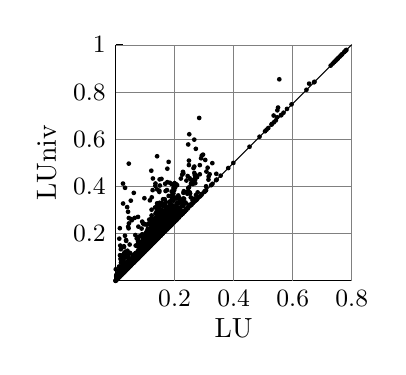
\begin{tikzpicture}

\draw (0,0) -- (3,0);
\node at (1.5,-0.6) {LU};
\node [anchor=north] at (0.75,0) {\small 0.2};
\draw (0.75,0) -- (0.75,0.1);
\draw [style=help lines] (0.75,0) -- (0.75,3);
\node [anchor=north] at (1.5,0) {\small 0.4};
\draw (1.5,0) -- (1.5,0.1);
\draw [style=help lines] (1.5,0) -- (1.5,3);
\node [anchor=north] at (2.25,0) {\small 0.6};
\draw (2.25,0) -- (2.25,0.1);
\draw [style=help lines] (2.25,0) -- (2.25,3);
\node [anchor=north] at (3,0) {\small 0.8};
\draw (3,0) -- (3,0.1);
\draw [style=help lines] (3,0) -- (3,3);
\draw (0,0) -- (0,3);
\node [rotate=90] at (-2.5em,1.5) {LUniv};
\node [anchor=east] at (0,0.599) {\small 0.2};
\draw (0,0.599) -- (0.1,0.599);
\draw [style=help lines] (0,0.599) -- (3,0.599);
\node [anchor=east] at (0,1.198) {\small 0.4};
\draw (0,1.198) -- (0.1,1.198);
\draw [style=help lines] (0,1.198) -- (3,1.198);
\node [anchor=east] at (0,1.797) {\small 0.6};
\draw (0,1.797) -- (0.1,1.797);
\draw [style=help lines] (0,1.797) -- (3,1.797);
\node [anchor=east] at (0,2.396) {\small 0.8};
\draw (0,2.396) -- (0.1,2.396);
\draw [style=help lines] (0,2.396) -- (3,2.396);
\node [anchor=east] at (0,2.995) {\small 1};
\draw (0,2.995) -- (0.1,2.995);
\draw [style=help lines] (0,2.995) -- (3,2.995);
\foreach \pos in {
	(0.000000, 0.000000),
	(0.005240, 0.005240),
	(0.010682, 0.010682),
	(0.015175, 0.015175),
	(0.019519, 0.019519),
	(0.011300, 0.029959),
	(0.019595, 0.028273),
	(0.024510, 0.024510),
	(0.011766, 0.037645),
	(0.028846, 0.028846),
	(0.019449, 0.038898),
	(0.030308, 0.035019),
	(0.036408, 0.036408),
	(0.034538, 0.043075),
	(0.041208, 0.041818),
	(0.008286, 0.060941),
	(0.043578, 0.047670),
	(0.039111, 0.053466),
	(0.049368, 0.050282),
	(0.022477, 0.068865),
	(0.016859, 0.071395),
	(0.010680, 0.074302),
	(0.054051, 0.054154),
	(0.046683, 0.066164),
	(0.058384, 0.058384),
	(0.039416, 0.078186),
	(0.060736, 0.064244),
	(0.055657, 0.072373),
	(0.046408, 0.081664),
	(0.065991, 0.067421),
	(0.052330, 0.079270),
	(0.059494, 0.078548),
	(0.065122, 0.073995),
	(0.027266, 0.096107),
	(0.070894, 0.071107),
	(0.066471, 0.080369),
	(0.057514, 0.087709),
	(0.074950, 0.075947),
	(0.049802, 0.095644),
	(0.041119, 0.099884),
	(0.065398, 0.086684),
	(0.073090, 0.082441),
	(0.079679, 0.079679),
	(0.065648, 0.093650),
	(0.073850, 0.088421),
	(0.054793, 0.102018),
	(0.043824, 0.107619),
	(0.060764, 0.100052),
	(0.080854, 0.086707),
	(0.067071, 0.102366),
	(0.086862, 0.086862),
	(0.081852, 0.094573),
	(0.050777, 0.114381),
	(0.074022, 0.103266),
	(0.089614, 0.092495),
	(0.068716, 0.109486),
	(0.081107, 0.100758),
	(0.061254, 0.115503),
	(0.087183, 0.098250),
	(0.054288, 0.119939),
	(0.038040, 0.126958),
	(0.095093, 0.095395),
	(0.083427, 0.108037),
	(0.093542, 0.101529),
	(0.079141, 0.113669),
	(0.072835, 0.118268),
	(0.045721, 0.131296),
	(0.099775, 0.099775),
	(0.070397, 0.124436),
	(0.090729, 0.111715),
	(0.097880, 0.106648),
	(0.087114, 0.116676),
	(0.002809, 0.146067),
	(0.079539, 0.123544),
	(0.104222, 0.104355),
	(0.095442, 0.116615),
	(0.102629, 0.110546),
	(0.072835, 0.132341),
	(0.108540, 0.108736),
	(0.092309, 0.123067),
	(0.086578, 0.128831),
	(0.104623, 0.116931),
	(0.112820, 0.113157),
	(0.093507, 0.132838),
	(0.111032, 0.119016),
	(0.104301, 0.127636),
	(0.117714, 0.118072),
	(0.093454, 0.139409),
	(0.110423, 0.126945),
	(0.103057, 0.135142),
	(0.116910, 0.124068),
	(0.123373, 0.123847),
	(0.111276, 0.135312),
	(0.117323, 0.130197),
	(0.124177, 0.129868),
	(0.119859, 0.137071),
	(0.068662, 0.169014),
	(0.089438, 0.160375),
	(0.116412, 0.142188),
	(0.095884, 0.156794),
	(0.130244, 0.130693),
	(0.045088, 0.180847),
	(0.126865, 0.137582),
	(0.061123, 0.179488),
	(0.134693, 0.134991),
	(0.111188, 0.156832),
	(0.121036, 0.149412),
	(0.131782, 0.141849),
	(0.096415, 0.168813),
	(0.117763, 0.155382),
	(0.138339, 0.140055),
	(0.080887, 0.181983),
	(0.133837, 0.148182),
	(0.140760, 0.146263),
	(0.129770, 0.156387),
	(0.101752, 0.178496),
	(0.140568, 0.152539),
	(0.124092, 0.166266),
	(0.146779, 0.147280),
	(0.147007, 0.153321),
	(0.112796, 0.180528),
	(0.144330, 0.160438),
	(0.108010, 0.187785),
	(0.130775, 0.173552),
	(0.153846, 0.153846),
	(0.138526, 0.170375),
	(0.151331, 0.160330),
	(0.116438, 0.189604),
	(0.148301, 0.166050),
	(0.159091, 0.159091),
	(0.153552, 0.169284),
	(0.159054, 0.166395),
	(0.132564, 0.189486),
	(0.150860, 0.176181),
	(0.094182, 0.213071),
	(0.166667, 0.166667),
	(0.161309, 0.174369),
	(0.146494, 0.188143),
	(0.068702, 0.230854),
	(0.168686, 0.172947),
	(0.124738, 0.207538),
	(0.160190, 0.182191),
	(0.077376, 0.230050),
	(0.116300, 0.214097),
	(0.166922, 0.179007),
	(0.131261, 0.208117),
	(0.173606, 0.177528),
	(0.159574, 0.194503),
	(0.174016, 0.184222),
	(0.179564, 0.180054),
	(0.165931, 0.193022),
	(0.171103, 0.189532),
	(0.120347, 0.225424),
	(0.161601, 0.200677),
	(0.076732, 0.246686),
	(0.179341, 0.188595),
	(0.185308, 0.185560),
	(0.176153, 0.194376),
	(0.132669, 0.231269),
	(0.182430, 0.195460),
	(0.190081, 0.190793),
	(0.084904, 0.257799),
	(0.072782, 0.261562),
	(0.175120, 0.207888),
	(0.189810, 0.198119),
	(0.194946, 0.194946),
	(0.185239, 0.208139),
	(0.171769, 0.219867),
	(0.191410, 0.206772),
	(0.197353, 0.201440),
	(0.094054, 0.265946),
	(0.147789, 0.241013),
	(0.062797, 0.278281),
	(0.161275, 0.235616),
	(0.184083, 0.219008),
	(0.154805, 0.241902),
	(0.202897, 0.203884),
	(0.192831, 0.218390),
	(0.205231, 0.212015),
	(0.103448, 0.280788),
	(0.192849, 0.230473),
	(0.206108, 0.219084),
	(0.212089, 0.214481),
	(0.185789, 0.241775),
	(0.204179, 0.229419),
	(0.172061, 0.255348),
	(0.215604, 0.222021),
	(0.210520, 0.228547),
	(0.222696, 0.224346),
	(0.212628, 0.234581),
	(0.219582, 0.230989),
	(0.193078, 0.254962),
	(0.228261, 0.228261),
	(0.216663, 0.239534),
	(0.168837, 0.276957),
	(0.133041, 0.296518),
	(0.056493, 0.323925),
	(0.233010, 0.233010),
	(0.194622, 0.268564),
	(0.203616, 0.264023),
	(0.228530, 0.245017),
	(0.236479, 0.238095),
	(0.087494, 0.324280),
	(0.212490, 0.262318),
	(0.204021, 0.270597),
	(0.210021, 0.268504),
	(0.236555, 0.245576),
	(0.231781, 0.250802),
	(0.242110, 0.242110),
	(0.134328, 0.318408),
	(0.230820, 0.257512),
	(0.209390, 0.275701),
	(0.241534, 0.249383),
	(0.247934, 0.247934),
	(0.223259, 0.272292),
	(0.237430, 0.260768),
	(0.160243, 0.314568),
	(0.218291, 0.277480),
	(0.229548, 0.270470),
	(0.243730, 0.258209),
	(0.234504, 0.266870),
	(0.250974, 0.253243),
	(0.249047, 0.261067),
	(0.242545, 0.269783),
	(0.254983, 0.258756),
	(0.218161, 0.292502),
	(0.240307, 0.276518),
	(0.252135, 0.266873),
	(0.260870, 0.260870),
	(0.220285, 0.298421),
	(0.111483, 0.356001),
	(0.260602, 0.268810),
	(0.250028, 0.282343),
	(0.239909, 0.291172),
	(0.258720, 0.275401),
	(0.215543, 0.313621),
	(0.269565, 0.269565),
	(0.272120, 0.275648),
	(0.136600, 0.362996),
	(0.265161, 0.284910),
	(0.243765, 0.303831),
	(0.270900, 0.281833),
	(0.126701, 0.369859),
	(0.260209, 0.293482),
	(0.277923, 0.278696),
	(0.234560, 0.316205),
	(0.222632, 0.326556),
	(0.270852, 0.289003),
	(0.277199, 0.286041),
	(0.252807, 0.307887),
	(0.185896, 0.352863),
	(0.282536, 0.282536),
	(0.268998, 0.301397),
	(0.282000, 0.289685),
	(0.246580, 0.321812),
	(0.066667, 0.400000),
	(0.288462, 0.288462),
	(0.151345, 0.381215),
	(0.278192, 0.301585),
	(0.283743, 0.296460),
	(0.239348, 0.336139),
	(0.291415, 0.294021),
	(0.287822, 0.302328),
	(0.280098, 0.310157),
	(0.296928, 0.296928),
	(0.276908, 0.318120),
	(0.294644, 0.304676),
	(0.283910, 0.317924),
	(0.301676, 0.301676),
	(0.292588, 0.311365),
	(0.275166, 0.328035),
	(0.301967, 0.308146),
	(0.289614, 0.320347),
	(0.073602, 0.429833),
	(0.255747, 0.353974),
	(0.307793, 0.309812),
	(0.299555, 0.317967),
	(0.285690, 0.331798),
	(0.291233, 0.327480),
	(0.106871, 0.428114),
	(0.276708, 0.344071),
	(0.299968, 0.325193),
	(0.312354, 0.314122),
	(0.295918, 0.331633),
	(0.285868, 0.340752),
	(0.310823, 0.322255),
	(0.305575, 0.327690),
	(0.316164, 0.319194),
	(0.286392, 0.347849),
	(0.060005, 0.446577),
	(0.106195, 0.438053),
	(0.305293, 0.333783),
	(0.296974, 0.343566),
	(0.322167, 0.322167),
	(0.312910, 0.331572),
	(0.312014, 0.338456),
	(0.322953, 0.328297),
	(0.322724, 0.335459),
	(0.328612, 0.332499),
	(0.322366, 0.341480),
	(0.313945, 0.350035),
	(0.335294, 0.335294),
	(0.329407, 0.343479),
	(0.292932, 0.375183),
	(0.285743, 0.380904),
	(0.339623, 0.339623),
	(0.329983, 0.349624),
	(0.318882, 0.364278),
	(0.338061, 0.347791),
	(0.312845, 0.371287),
	(0.333521, 0.355283),
	(0.344828, 0.344828),
	(0.329449, 0.363087),
	(0.304328, 0.385979),
	(0.345023, 0.351445),
	(0.179221, 0.459740),
	(0.318407, 0.379002),
	(0.351668, 0.351889),
	(0.328883, 0.375662),
	(0.333916, 0.372378),
	(0.347110, 0.360178),
	(0.314085, 0.393774),
	(0.354966, 0.357565),
	(0.332132, 0.381081),
	(0.351485, 0.364355),
	(0.324842, 0.389943),
	(0.344225, 0.376216),
	(0.350975, 0.371407),
	(0.357579, 0.367012),
	(0.338266, 0.385928),
	(0.362903, 0.362903),
	(0.318905, 0.402705),
	(0.255998, 0.446698),
	(0.352830, 0.378469),
	(0.284342, 0.433524),
	(0.347052, 0.385355),
	(0.361687, 0.372061),
	(0.367220, 0.367220),
	(0.343659, 0.394324),
	(0.134967, 0.506459),
	(0.368543, 0.373169),
	(0.356720, 0.384911),
	(0.331017, 0.408341),
	(0.351659, 0.392818),
	(0.365693, 0.380502),
	(0.375000, 0.375000),
	(0.362288, 0.388213),
	(0.277903, 0.453184),
	(0.352840, 0.399245),
	(0.134050, 0.515837),
	(0.327966, 0.420763),
	(0.343766, 0.408247),
	(0.374287, 0.383005),
	(0.047966, 0.534272),
	(0.367765, 0.391561),
	(0.363360, 0.395749),
	(0.380486, 0.382499),
	(0.288200, 0.456127),
	(0.374979, 0.389055),
	(0.359994, 0.403423),
	(0.368080, 0.399501),
	(0.374610, 0.395624),
	(0.356955, 0.412073),
	(0.351058, 0.417581),
	(0.319725, 0.443578),
	(0.381292, 0.392313),
	(0.386757, 0.389393),
	(0.367185, 0.409175),
	(0.372944, 0.404971),
	(0.381582, 0.399003),
	(0.353678, 0.425519),
	(0.335780, 0.440367),
	(0.363539, 0.418231),
	(0.390437, 0.394896),
	(0.371535, 0.413705),
	(0.388458, 0.402624),
	(0.381140, 0.409792),
	(0.366476, 0.424258),
	(0.396476, 0.396476),
	(0.372454, 0.421855),
	(0.328851, 0.458011),
	(0.353040, 0.441721),
	(0.381510, 0.417440),
	(0.397622, 0.402422),
	(0.365122, 0.432293),
	(0.390487, 0.412215),
	(0.403525, 0.403525),
	(0.342625, 0.457296),
	(0.399156, 0.409006),
	(0.365000, 0.440000),
	(0.384257, 0.424034),
	(0.286160, 0.496449),
	(0.394019, 0.417766),
	(0.406413, 0.410487),
	(0.401840, 0.415068),
	(0.384509, 0.431813),
	(0.393909, 0.425888),
	(0.352988, 0.461174),
	(0.400215, 0.421194),
	(0.375286, 0.445128),
	(0.408177, 0.416884),
	(0.119683, 0.571497),
	(0.368411, 0.455178),
	(0.400448, 0.428297),
	(0.415065, 0.415065),
	(0.394568, 0.434711),
	(0.387655, 0.442274),
	(0.357555, 0.468446),
	(0.409794, 0.423679),
	(0.369574, 0.461087),
	(0.355698, 0.474212),
	(0.396590, 0.440710),
	(0.382935, 0.453856),
	(0.377818, 0.458562),
	(0.416193, 0.424197),
	(0.412021, 0.430581),
	(0.389075, 0.451667),
	(0.406718, 0.435862),
	(0.421696, 0.421696),
	(0.395029, 0.448501),
	(0.345883, 0.487517),
	(0.402098, 0.444026),
	(0.288142, 0.525596),
	(0.335767, 0.498043),
	(0.269341, 0.537021),
	(0.353271, 0.485981),
	(0.421797, 0.429285),
	(0.412102, 0.438682),
	(0.384078, 0.463439),
	(0.375463, 0.471799),
	(0.395371, 0.456070),
	(0.418929, 0.437548),
	(0.427790, 0.430375),
	(0.413434, 0.444786),
	(0.408596, 0.449698),
	(0.390287, 0.466856),
	(0.403968, 0.455966),
	(0.399324, 0.461363),
	(0.419853, 0.443551),
	(0.367646, 0.488728),
	(0.428137, 0.437268),
	(0.433735, 0.433735),
	(0.356256, 0.499704),
	(0.386041, 0.477485),
	(0.414499, 0.455458),
	(0.421738, 0.449641),
	(0.427825, 0.444914),
	(0.404006, 0.468046),
	(0.435175, 0.440248),
	(0.279097, 0.553735),
	(0.414312, 0.461461),
	(0.376077, 0.493780),
	(0.401504, 0.473584),
	(0.410092, 0.466514),
	(0.388599, 0.484690),
	(0.427583, 0.451639),
	(0.434366, 0.446543),
	(0.423053, 0.458473),
	(0.441176, 0.441176),
	(0.412704, 0.472595),
	(0.429199, 0.457739),
	(0.417742, 0.468725),
	(0.439795, 0.449539),
	(0.445946, 0.445946),
	(0.410009, 0.479950),
	(0.427404, 0.466149),
	(0.403310, 0.487155),
	(0.251356, 0.580379),
	(0.436267, 0.458411),
	(0.444079, 0.454294),
	(0.373795, 0.514102),
	(0.399655, 0.494909),
	(0.420345, 0.477706),
	(0.426013, 0.473091),
	(0.380873, 0.511259),
	(0.436780, 0.464843),
	(0.388486, 0.505994),
	(0.411698, 0.488848),
	(0.349836, 0.535075),
	(0.442851, 0.462218),
	(0.366551, 0.525130),
	(0.395959, 0.503830),
	(0.453265, 0.453265),
	(0.432213, 0.474326),
	(0.448926, 0.460234),
	(0.307100, 0.564969),
	(0.427919, 0.482331),
	(0.408273, 0.500000),
	(0.443300, 0.469350),
	(0.387109, 0.517904),
	(0.440752, 0.475887),
	(0.422222, 0.492832),
	(0.458113, 0.459752),
	(0.434211, 0.483083),
	(0.344677, 0.550611),
	(0.453209, 0.465377),
	(0.429816, 0.489593),
	(0.407727, 0.508388),
	(0.383030, 0.529256),
	(0.450694, 0.474190),
	(0.459262, 0.465945),
	(0.426174, 0.497742),
	(0.438524, 0.487418),
	(0.420582, 0.503356),
	(0.444861, 0.482141),
	(0.389500, 0.529957),
	(0.398489, 0.524159),
	(0.456694, 0.475693),
	(0.419703, 0.509593),
	(0.413846, 0.515996),
	(0.445082, 0.489344),
	(0.428371, 0.504090),
	(0.466664, 0.471510),
	(0.407631, 0.524096),
	(0.440126, 0.498141),
	(0.457911, 0.481880),
	(0.463374, 0.477187),
	(0.420221, 0.515977),
	(0.448663, 0.494269),
	(0.398023, 0.536590),
	(0.370987, 0.557241),
	(0.054669, 0.667251),
	(0.456791, 0.489939),
	(0.473684, 0.473684),
	(0.426296, 0.516821),
	(0.446224, 0.500494),
	(0.420713, 0.522581),
	(0.469959, 0.478806),
	(0.465053, 0.483614),
	(0.380460, 0.552874),
	(0.434279, 0.512449),
	(0.386355, 0.549636),
	(0.353282, 0.571911),
	(0.444094, 0.507402),
	(0.404828, 0.539390),
	(0.417613, 0.530333),
	(0.454109, 0.499583),
	(0.470187, 0.486797),
	(0.395304, 0.549832),
	(0.344029, 0.584753),
	(0.442215, 0.515249),
	(0.426866, 0.528668),
	(0.338417, 0.589688),
	(0.467150, 0.494051),
	(0.437385, 0.520606),
	(0.409775, 0.543261),
	(0.477288, 0.485239),
	(0.463126, 0.499091),
	(0.454806, 0.507038),
	(0.449595, 0.514166),
	(0.399448, 0.555249),
	(0.476725, 0.491325),
	(0.484305, 0.484305),
	(0.472477, 0.497534),
	(0.166063, 0.665804),
	(0.462603, 0.507468),
	(0.428959, 0.537557),
	(0.438565, 0.530045),
	(0.482922, 0.491077),
	(0.406012, 0.556445),
	(0.378086, 0.576873),
	(0.387984, 0.570282),
	(0.448464, 0.524297),
	(0.460861, 0.514221),
	(0.414800, 0.553367),
	(0.489474, 0.489474),
	(0.472714, 0.506145),
	(0.481150, 0.498403),
	(0.467116, 0.512856),
	(0.438624, 0.538311),
	(0.458882, 0.522949),
	(0.487994, 0.496340),
	(0.422147, 0.554068),
	(0.451424, 0.531566),
	(0.466053, 0.519211),
	(0.482041, 0.504601),
	(0.475019, 0.512063),
	(0.444805, 0.539502),
	(0.432977, 0.549132),
	(0.489493, 0.502707),
	(0.460006, 0.530072),
	(0.481091, 0.511249),
	(0.465807, 0.525766),
	(0.497326, 0.497326),
	(0.403694, 0.576517),
	(0.159934, 0.686681),
	(0.488030, 0.509051),
	(0.476989, 0.520096),
	(0.444739, 0.549967),
	(0.460177, 0.537409),
	(0.486034, 0.514765),
	(0.472866, 0.527296),
	(0.497433, 0.504315),
	(0.457496, 0.542903),
	(0.466667, 0.535897),
	(0.453172, 0.547424),
	(0.481420, 0.524284),
	(0.495560, 0.511895),
	(0.504621, 0.504621),
	(0.491354, 0.518012),
	(0.422150, 0.575829),
	(0.381960, 0.603662),
	(0.448529, 0.556415),
	(0.465848, 0.542817),
	(0.474676, 0.536808),
	(0.483137, 0.531032),
	(0.488706, 0.526382),
	(0.501141, 0.515319),
	(0.391802, 0.602887),
	(0.506565, 0.510464),
	(0.447001, 0.564165),
	(0.495734, 0.522184),
	(0.439750, 0.570162),
	(0.465054, 0.551075),
	(0.489160, 0.532700),
	(0.453099, 0.563833),
	(0.458772, 0.559334),
	(0.405253, 0.599437),
	(0.474568, 0.546480),
	(0.495307, 0.528279),
	(0.483460, 0.539447),
	(0.504248, 0.520792),
	(0.450341, 0.570564),
	(0.512746, 0.515520),
	(0.441860, 0.577519),
	(0.501491, 0.527336),
	(0.458567, 0.566420),
	(0.492781, 0.538644),
	(0.424528, 0.594340),
	(0.471543, 0.558511),
	(0.418421, 0.600000),
	(0.511430, 0.523187),
	(0.485981, 0.548910),
	(0.518433, 0.518433),
	(0.481172, 0.553771),
	(0.397163, 0.617021),
	(0.507797, 0.529994),
	(0.499890, 0.538954),
	(0.492979, 0.545383),
	(0.463744, 0.571388),
	(0.470496, 0.565913),
	(0.518449, 0.525126),
	(0.506655, 0.537048),
	(0.513841, 0.530709),
	(0.480680, 0.562007),
	(0.499875, 0.545215),
	(0.462379, 0.578394),
	(0.331114, 0.662437),
	(0.469006, 0.575661),
	(0.445518, 0.594303),
	(0.478049, 0.568502),
	(0.459224, 0.584323),
	(0.497271, 0.553289),
	(0.418306, 0.615269),
	(0.522380, 0.530165),
	(0.510367, 0.542434),
	(0.506413, 0.547373),
	(0.484951, 0.566576),
	(0.397803, 0.630860),
	(0.492844, 0.560050),
	(0.290155, 0.687392),
	(0.516544, 0.538655),
	(0.441176, 0.603209),
	(0.170160, 0.728239),
	(0.525012, 0.535945),
	(0.516448, 0.544798),
	(0.459983, 0.593934),
	(0.502470, 0.559048),
	(0.498127, 0.563670),
	(0.507692, 0.555944),
	(0.470588, 0.587688),
	(0.530871, 0.534179),
	(0.446188, 0.607419),
	(0.420966, 0.625258),
	(0.453385, 0.603492),
	(0.525364, 0.542567),
	(0.484816, 0.579582),
	(0.514877, 0.553378),
	(0.490400, 0.575425),
	(0.522716, 0.549034),
	(0.506852, 0.565146),
	(0.536817, 0.536817),
	(0.497461, 0.573631),
	(0.479582, 0.588863),
	(0.513340, 0.560134),
	(0.531625, 0.543286),
	(0.439744, 0.621249),
	(0.520462, 0.557416),
	(0.478368, 0.595382),
	(0.494804, 0.582300),
	(0.512714, 0.566824),
	(0.531265, 0.549866),
	(0.538288, 0.543919),
	(0.448388, 0.621016),
	(0.527366, 0.556160),
	(0.519075, 0.564162),
	(0.505263, 0.577346),
	(0.510781, 0.573589),
	(0.488704, 0.592866),
	(0.538662, 0.550565),
	(0.533609, 0.555762),
	(0.517988, 0.571085),
	(0.544416, 0.548223),
	(0.506223, 0.583740),
	(0.524941, 0.567103),
	(0.498891, 0.592018),
	(0.480561, 0.607290),
	(0.490469, 0.599682),
	(0.427754, 0.646207),
	(0.531491, 0.564200),
	(0.539521, 0.556925),
	(0.519775, 0.576993),
	(0.409250, 0.660477),
	(0.515587, 0.582903),
	(0.550459, 0.550459),
	(0.546159, 0.555842),
	(0.505885, 0.592938),
	(0.498000, 0.600000),
	(0.421376, 0.656250),
	(0.486091, 0.610542),
	(0.467240, 0.625134),
	(0.540944, 0.562804),
	(0.530404, 0.573327),
	(0.536018, 0.569052),
	(0.459993, 0.632625),
	(0.514647, 0.589871),
	(0.527634, 0.578931),
	(0.504593, 0.600570),
	(0.522558, 0.585477),
	(0.479373, 0.621932),
	(0.550669, 0.560229),
	(0.510108, 0.597834),
	(0.468154, 0.631711),
	(0.500924, 0.607341),
	(0.547765, 0.566442),
	(0.534532, 0.579185),
	(0.531276, 0.584459),
	(0.494881, 0.616041),
	(0.520033, 0.596688),
	(0.554101, 0.565653),
	(0.545618, 0.574430),
	(0.541957, 0.580127),
	(0.510227, 0.609784),
	(0.205927, 0.768141),
	(0.552677, 0.572280),
	(0.538497, 0.585649),
	(0.491003, 0.627064),
	(0.524541, 0.600768),
	(0.560160, 0.568182),
	(0.534068, 0.593215),
	(0.502039, 0.620588),
	(0.548518, 0.580863),
	(0.519449, 0.608075),
	(0.459538, 0.656792),
	(0.541717, 0.591048),
	(0.556522, 0.578435),
	(0.475697, 0.647809),
	(0.548655, 0.587413),
	(0.528308, 0.606592),
	(0.502244, 0.628581),
	(0.362491, 0.718310),
	(0.568895, 0.569220),
	(0.554201, 0.584688),
	(0.537880, 0.600000),
	(0.452985, 0.666602),
	(0.496946, 0.634647),
	(0.487500, 0.642188),
	(0.520767, 0.615914),
	(0.508745, 0.625936),
	(0.201149, 0.781609),
	(0.349315, 0.727984),
	(0.526292, 0.613469),
	(0.565823, 0.577215),
	(0.375103, 0.717302),
	(0.560847, 0.584127),
	(0.549990, 0.594403),
	(0.555380, 0.590981),
	(0.503226, 0.636774),
	(0.534977, 0.610704),
	(0.543813, 0.604739),
	(0.575218, 0.575218),
	(0.493238, 0.647806),
	(0.169014, 0.797007),
	(0.561943, 0.590272),
	(0.550836, 0.601535),
	(0.555566, 0.597645),
	(0.398352, 0.712454),
	(0.522885, 0.627023),
	(0.530423, 0.621693),
	(0.540895, 0.613421),
	(0.490391, 0.654510),
	(0.503092, 0.644962),
	(0.570152, 0.586522),
	(0.576300, 0.582188),
	(0.520157, 0.634218),
	(0.537706, 0.620457),
	(0.566623, 0.594345),
	(0.561712, 0.599207),
	(0.484232, 0.663784),
	(0.528721, 0.629243),
	(0.557440, 0.603974),
	(0.476589, 0.669732),
	(0.550344, 0.610756),
	(0.575707, 0.588934),
	(0.545394, 0.617628),
	(0.338735, 0.751176),
	(0.449843, 0.691017),
	(0.513295, 0.647399),
	(0.526993, 0.636575),
	(0.493912, 0.663051),
	(0.504110, 0.656621),
	(0.554594, 0.615180),
	(0.562745, 0.608140),
	(0.573012, 0.598590),
	(0.568468, 0.603400),
	(0.547612, 0.623404),
	(0.471544, 0.682949),
	(0.522961, 0.646677),
	(0.581413, 0.594796),
	(0.587486, 0.589112),
	(0.560727, 0.615273),
	(0.494479, 0.670741),
	(0.532982, 0.641161),
	(0.242647, 0.798291),
	(0.542477, 0.635107),
	(0.572501, 0.608653),
	(0.459081, 0.698711),
	(0.478803, 0.685786),
	(0.558140, 0.623477),
	(0.580630, 0.603137),
	(0.588208, 0.598035),
	(0.539308, 0.642558),
	(0.549115, 0.634896),
	(0.571909, 0.616387),
	(0.451627, 0.709328),
	(0.459040, 0.704798),
	(0.567445, 0.621271),
	(0.595479, 0.595479),
	(0.577864, 0.612816),
	(0.545763, 0.641808),
	(0.423430, 0.728619),
	(0.467313, 0.701843),
	(0.513117, 0.669753),
	(0.440383, 0.720431),
	(0.564108, 0.628541),
	(0.588454, 0.606167),
	(0.536747, 0.652916),
	(0.523415, 0.665111),
	(0.575342, 0.622227),
	(0.585569, 0.612701),
	(0.555939, 0.640217),
	(0.499266, 0.685941),
	(0.474840, 0.704026),
	(0.535206, 0.659978),
	(0.572127, 0.628973),
	(0.581463, 0.620658),
	(0.543146, 0.655380),
	(0.593545, 0.610281),
	(0.564638, 0.637860),
	(0.512202, 0.680693),
	(0.522266, 0.675766),
	(0.571379, 0.635367),
	(0.604290, 0.604290),
	(0.553432, 0.651316),
	(0.461397, 0.719724),
	(0.497370, 0.695649),
	(0.588977, 0.621472),
	(0.503515, 0.693322),
	(0.533891, 0.670335),
	(0.584343, 0.627213),
	(0.566957, 0.643478),
	(0.494592, 0.701549),
	(0.601018, 0.613102),
	(0.546484, 0.662577),
	(0.285501, 0.810885),
	(0.580300, 0.634513),
	(0.520321, 0.685175),
	(0.554206, 0.658879),
	(0.501828, 0.700640),
	(0.561576, 0.655172),
	(0.458852, 0.731146),
	(0.586552, 0.633763),
	(0.595937, 0.626411),
	(0.546581, 0.670108),
	(0.606158, 0.616742),
	(0.570272, 0.650809),
	(0.538013, 0.677938),
	(0.485914, 0.717472),
	(0.561986, 0.661590),
	(0.535222, 0.684533),
	(0.583099, 0.645504),
	(0.570204, 0.657020),
	(0.599842, 0.631059),
	(0.556269, 0.671813),
	(0.483871, 0.725806),
	(0.517595, 0.702597),
	(0.589891, 0.644274),
	(0.605714, 0.629467),
	(0.595849, 0.639833),
	(0.580212, 0.655674),
	(0.549431, 0.682415),
	(0.568291, 0.667124),
	(0.613885, 0.626714),
	(0.605985, 0.635910),
	(0.576060, 0.663473),
	(0.516447, 0.712365),
	(0.588350, 0.655340),
	(0.532701, 0.701439),
	(0.623463, 0.623463),
	(0.567010, 0.677835),
	(0.599459, 0.649526),
	(0.608743, 0.641366),
	(0.620785, 0.629982),
	(0.596099, 0.654607),
	(0.560584, 0.685401),
	(0.530904, 0.709329),
	(0.584834, 0.666898),
	(0.428571, 0.776978),
	(0.545141, 0.700895),
	(0.618032, 0.638180),
	(0.608434, 0.648594),
	(0.595612, 0.661093),
	(0.464188, 0.759253),
	(0.552746, 0.697472),
	(0.158850, 0.875946),
	(0.604552, 0.654266),
	(0.626846, 0.633557),
	(0.579553, 0.677316),
	(0.563337, 0.692070),
	(0.525145, 0.722437),
	(0.570322, 0.688319),
	(0.575216, 0.684340),
	(0.593852, 0.668374),
	(0.588298, 0.673675),
	(0.559394, 0.697965),
	(0.619850, 0.645651),
	(0.633533, 0.634263),
	(0.613934, 0.653728),
	(0.519514, 0.732871),
	(0.583618, 0.683569),
	(0.574481, 0.693133),
	(0.602899, 0.669478),
	(0.594974, 0.676950),
	(0.624494, 0.650203),
	(0.612457, 0.662944),
	(0.631676, 0.648341),
	(0.574100, 0.700302),
	(0.544696, 0.725629),
	(0.588727, 0.692415),
	(0.610106, 0.673737),
	(0.455176, 0.787558),
	(0.483852, 0.770933),
	(0.509766, 0.754395),
	(0.583557, 0.699118),
	(0.617126, 0.670475),
	(0.630114, 0.658345),
	(0.571200, 0.710400),
	(0.600000, 0.686724),
	(0.639512, 0.650216),
	(0.605982, 0.682095),
	(0.527066, 0.746439),
	(0.551951, 0.729853),
	(0.612438, 0.680036),
	(0.596203, 0.696203),
	(0.621049, 0.675234),
	(0.487373, 0.777922),
	(0.629139, 0.668874),
	(0.590861, 0.703519),
	(0.610973, 0.686617),
	(0.605332, 0.692202),
	(0.650794, 0.650794),
	(0.644759, 0.659056),
	(0.536591, 0.750186),
	(0.564298, 0.730476),
	(0.498410, 0.777424),
	(0.503932, 0.774772),
	(0.605264, 0.700492),
	(0.579333, 0.722243),
	(0.652408, 0.657178),
	(0.597691, 0.707364),
	(0.558927, 0.738786),
	(0.639686, 0.670628),
	(0.621571, 0.688591),
	(0.573892, 0.729363),
	(0.631423, 0.683139),
	(0.551424, 0.750000),
	(0.658537, 0.658537),
	(0.620123, 0.695959),
	(0.609756, 0.705366),
	(0.561298, 0.746394),
	(0.528633, 0.770549),
	(0.496420, 0.792363),
	(0.578493, 0.735811),
	(0.617439, 0.706049),
	(0.591578, 0.727941),
	(0.650068, 0.677564),
	(0.601297, 0.721232),
	(0.553009, 0.760116),
	(0.503860, 0.793657),
	(0.641108, 0.687776),
	(0.610619, 0.716814),
	(0.534387, 0.776022),
	(0.626902, 0.703763),
	(0.633333, 0.700000),
	(0.510000, 0.795000),
	(0.568756, 0.754911),
	(0.147613, 0.935419),
	(0.620726, 0.715323),
	(0.457867, 0.829110),
	(0.654673, 0.686406),
	(0.612920, 0.724430),
	(0.578804, 0.752038),
	(0.542079, 0.779703),
	(0.630105, 0.710618),
	(0.642763, 0.700662),
	(0.592557, 0.743615),
	(0.575581, 0.758721),
	(0.673825, 0.673825),
	(0.652038, 0.695925),
	(0.531626, 0.792061),
	(0.599849, 0.744796),
	(0.574570, 0.765774),
	(0.659663, 0.694467),
	(0.674079, 0.681241),
	(0.532776, 0.798025),
	(0.655954, 0.701001),
	(0.616354, 0.737674),
	(0.641967, 0.715720),
	(0.633417, 0.724492),
	(0.561127, 0.782535),
	(0.670298, 0.691945),
	(0.595715, 0.757296),
	(0.576335, 0.772787),
	(0.550445, 0.792810),
	(0.630107, 0.731350),
	(0.682916, 0.682916),
	(0.660194, 0.705502),
	(0.528027, 0.810538),
	(0.652057, 0.717127),
	(0.680948, 0.692803),
	(0.564191, 0.790897),
	(0.610321, 0.757195),
	(0.649779, 0.725324),
	(0.659559, 0.716912),
	(0.643096, 0.732183),
	(0.575342, 0.789041),
	(0.679777, 0.702067),
	(0.600244, 0.771394),
	(0.657934, 0.724052),
	(0.667195, 0.717908),
	(0.693531, 0.693531),
	(0.580715, 0.793283),
	(0.681051, 0.709193),
	(0.609070, 0.772101),
	(0.546601, 0.817641),
	(0.095866, 0.980783),
	(0.592294, 0.788632),
	(0.553834, 0.817292),
	(0.656421, 0.737753),
	(0.577739, 0.802079),
	(0.698598, 0.700185),
	(0.665834, 0.732418),
	(0.646341, 0.750000),
	(0.507137, 0.850912),
	(0.654026, 0.744949),
	(0.608888, 0.783419),
	(0.537012, 0.834993),
	(0.679064, 0.725024),
	(0.641829, 0.758479),
	(0.623302, 0.775467),
	(0.704626, 0.704626),
	(0.619914, 0.783726),
	(0.695884, 0.718554),
	(0.679642, 0.734963),
	(0.704590, 0.713883),
	(0.643585, 0.769799),
	(0.710526, 0.710526),
	(0.679426, 0.741627),
	(0.606784, 0.802764),
	(0.561753, 0.836653),
	(0.665811, 0.756895),
	(0.714844, 0.714844),
	(0.518086, 0.868145),
	(0.457605, 0.901973),
	(0.641938, 0.783812),
	(0.581733, 0.830445),
	(0.678832, 0.754745),
	(0.662606, 0.770808),
	(0.532624, 0.868475),
	(0.704585, 0.737860),
	(0.669867, 0.771787),
	(0.702280, 0.744599),
	(0.609656, 0.824059),
	(0.632091, 0.807131),
	(0.532115, 0.879831),
	(0.546667, 0.874545),
	(0.525787, 0.887456),
	(0.660095, 0.792687),
	(0.628592, 0.818718),
	(0.695622, 0.763477),
	(0.711300, 0.750490),
	(0.193795, 1.017425),
	(0.673267, 0.787129),
	(0.568203, 0.869585),
	(0.701840, 0.766053),
	(0.621918, 0.832877),
	(0.693942, 0.775332),
	(0.735849, 0.735849),
	(0.588889, 0.858586),
	(0.553130, 0.884836),
	(0.671505, 0.799847),
	(0.736598, 0.742049),
	(0.636111, 0.830556),
	(0.687275, 0.788742),
	(0.586462, 0.869481),
	(0.619427, 0.847864),
	(0.728682, 0.757967),
	(0.705292, 0.779944),
	(0.652568, 0.827795),
	(0.745968, 0.745968),
	(0.644153, 0.836190),
	(0.635945, 0.843318),
	(0.596037, 0.873418),
	(0.502131, 0.930744),
	(0.704850, 0.791445),
	(0.717991, 0.781703),
	(0.673004, 0.823194),
	(0.657279, 0.838332),
	(0.615364, 0.872058),
	(0.628131, 0.863198),
	(0.726146, 0.783913),
	(0.748756, 0.764041),
	(0.712975, 0.799177),
	(0.582252, 0.899844),
	(0.738182, 0.777940),
	(0.612713, 0.882963),
	(0.547723, 0.924950),
	(0.738570, 0.784291),
	(0.677468, 0.838983),
	(0.762520, 0.762520),
	(0.713451, 0.809079),
	(0.643332, 0.869296),
	(0.527973, 0.945629),
	(0.660185, 0.860608),
	(0.766803, 0.767580),
	(0.690101, 0.840527),
	(0.705574, 0.827869),
	(0.675773, 0.852726),
	(0.727800, 0.813987),
	(0.670419, 0.862275),
	(0.772954, 0.773229),
	(0.756048, 0.792339),
	(0.657288, 0.878690),
	(0.778086, 0.778086),
	(0.561170, 0.946809),
	(0.701356, 0.849762),
	(0.736622, 0.824288),
	(0.661900, 0.888662),
	(0.646434, 0.901366),
	(0.436185, 1.020918),
	(0.366460, 1.048137),
	(0.786268, 0.786956),
	(0.725703, 0.845783),
	(0.527840, 0.983853),
	(0.704651, 0.866512),
	(0.732973, 0.845897),
	(0.636136, 0.922208),
	(0.698451, 0.877783),
	(0.727380, 0.854052),
	(0.606766, 0.944420),
	(0.783197, 0.807649),
	(0.704707, 0.877981),
	(0.604639, 0.952577),
	(0.674676, 0.905334),
	(0.668944, 0.911180),
	(0.802867, 0.802867),
	(0.765521, 0.840332),
	(0.559630, 0.990115),
	(0.721584, 0.880023),
	(0.231947, 1.115987),
	(0.759238, 0.850451),
	(0.771832, 0.839166),
	(0.699438, 0.901685),
	(0.653558, 0.936224),
	(0.605996, 0.969412),
	(0.808431, 0.808431),
	(0.629630, 0.961353),
	(0.585608, 0.988921),
	(0.692866, 0.917775),
	(0.776657, 0.848363),
	(0.459691, 1.059605),
	(0.768138, 0.865451),
	(0.762579, 0.880544),
	(0.718232, 0.917127),
	(0.689311, 0.942557),
	(0.813210, 0.841901),
	(0.767702, 0.886957),
	(0.832173, 0.832173),
	(0.766972, 0.899515),
	(0.815785, 0.857660),
	(0.687773, 0.963974),
	(0.639608, 0.999164),
	(0.120569, 1.180296),
	(0.739935, 0.930125),
	(0.782743, 0.895181),
	(0.719048, 0.952381),
	(0.762915, 0.922906),
	(0.603359, 1.035186),
	(0.725449, 0.956705),
	(0.849656, 0.849656),
	(0.706407, 0.974930),
	(0.769209, 0.926295),
	(0.842355, 0.866307),
	(0.854533, 0.854533),
	(0.625489, 1.035215),
	(0.817721, 0.904457),
	(0.790231, 0.930222),
	(0.691446, 1.007637),
	(0.815476, 0.910714),
	(0.774580, 0.945848),
	(0.860457, 0.869976),
	(0.847835, 0.887930),
	(0.870518, 0.870518),
	(0.818750, 0.920536),
	(0.773868, 0.963799),
	(0.094626, 1.234003),
	(0.470780, 1.150833),
	(0.882141, 0.882141),
	(0.778312, 0.986273),
	(0.736239, 1.018349),
	(0.555253, 1.128470),
	(0.889960, 0.894887),
	(0.836842, 0.947368),
	(0.716900, 1.043057),
	(0.887892, 0.905830),
	(0.674505, 1.077970),
	(0.800264, 0.988445),
	(0.899462, 0.899462),
	(0.556432, 1.143983),
	(0.527619, 1.160000),
	(0.862767, 0.951340),
	(0.727721, 1.061652),
	(0.819113, 0.994198),
	(0.750000, 1.056641),
	(0.919260, 0.919260),
	(0.778462, 1.043077),
	(0.915152, 0.927273),
	(0.635748, 1.139472),
	(0.718872, 1.090055),
	(0.505191, 1.205109),
	(0.782450, 1.049360),
	(0.773585, 1.056604),
	(0.813528, 1.031079),
	(0.871802, 0.990304),
	(0.838608, 1.018987),
	(0.878970, 0.985761),
	(0.653403, 1.151309),
	(0.936771, 0.944138),
	(0.806592, 1.058977),
	(0.735849, 1.111140),
	(0.889187, 0.993865),
	(0.563484, 1.209601),
	(0.507280, 1.235027),
	(0.926209, 0.963104),
	(0.851545, 1.031128),
	(0.712614, 1.133940),
	(0.796258, 1.083601),
	(0.942477, 0.959673),
	(0.951758, 0.955726),
	(0.860312, 1.045138),
	(0.869859, 1.040416),
	(0.965509, 0.965509),
	(0.961968, 0.975487),
	(0.745174, 1.150579),
	(0.474447, 1.298975),
	(0.630553, 1.231853),
	(0.735981, 1.177570),
	(0.982973, 0.986654),
	(0.559671, 1.287184),
	(0.756113, 1.183567),
	(0.862017, 1.116076),
	(0.996406, 1.001797),
	(0.657224, 1.252125),
	(0.977296, 1.023469),
	(0.712938, 1.227089),
	(0.583070, 1.293901),
	(0.689524, 1.244712),
	(0.955359, 1.058749),
	(0.867100, 1.137546),
	(0.911253, 1.105215),
	(1.012376, 1.014299),
	(0.985358, 1.041089),
	(0.754455, 1.223762),
	(0.781395, 1.213953),
	(0.771084, 1.224900),
	(0.749203, 1.240170),
	(1.025563, 1.025563),
	(0.911917, 1.132124),
	(0.945552, 1.105938),
	(1.031007, 1.031759),
	(0.945510, 1.113017),
	(0.940929, 1.124444),
	(0.454321, 1.397531),
	(1.037037, 1.047009),
	(1.043449, 1.046800),
	(1.021382, 1.088816),
	(0.923607, 1.176910),
	(0.168363, 1.487512),
	(0.932798, 1.185557),
	(1.067554, 1.067554),
	(1.077793, 1.077793),
	(1.043199, 1.122754),
	(0.829296, 1.298091),
	(1.092965, 1.092965),
	(1.094572, 1.103053),
	(0.899847, 1.272554),
	(0.956877, 1.231227),
	(0.657758, 1.422945),
	(0.982147, 1.228258),
	(0.987500, 1.247917),
	(0.846984, 1.347799),
	(1.127451, 1.127451),
	(0.961497, 1.278742),
	(1.012681, 1.239141),
	(1.132105, 1.135807),
	(0.978145, 1.272298),
	(0.941359, 1.302524),
	(1.140000, 1.140000),
	(0.861057, 1.363014),
	(0.916232, 1.329549),
	(1.149254, 1.149254),
	(0.856120, 1.382884),
	(1.011202, 1.284114),
	(1.006897, 1.300000),
	(0.674399, 1.509743),
	(1.149648, 1.199312),
	(0.527811, 1.581065),
	(1.036226, 1.316350),
	(1.006639, 1.342186),
	(1.019659, 1.340105),
	(1.001081, 1.369142),
	(1.213568, 1.213568),
	(1.070234, 1.351802),
	(0.931723, 1.469478),
	(0.990041, 1.431089),
	(1.230914, 1.230914),
	(1.180322, 1.283272),
	(1.000311, 1.450218),
	(1.182295, 1.324041),
	(0.932359, 1.525974),
	(1.154213, 1.386725),
	(1.195140, 1.353093),
	(1.277256, 1.277256),
	(1.284738, 1.284738),
	(1.070503, 1.468345),
	(1.169483, 1.435660),
	(1.279526, 1.358386),
	(1.334648, 1.334648),
	(1.086285, 1.555649),
	(1.139263, 1.534387),
	(1.095506, 1.589994),
	(1.229111, 1.493686),
	(1.110901, 1.601780),
	(0.922850, 1.730713),
	(1.019751, 1.675551),
	(1.431364, 1.431364),
	(1.000112, 1.792195),
	(0.936129, 1.860556),
	(1.496431, 1.496431),
	(1.062274, 2.067675),
	(1.701794, 1.701794),
	(1.828887, 1.828982),
	(1.898836, 1.898836),
	(1.918677, 1.918677),
	(1.940049, 1.940049),
	(1.981150, 1.983004),
	(1.984119, 1.990266),
	(2.011980, 2.012108),
	(2.035787, 2.036799),
	(2.007715, 2.098120),
	(2.052773, 2.076303),
	(2.100806, 2.101230),
	(2.105910, 2.105910),
	(2.055030, 2.164416),
	(2.064048, 2.199786),
	(2.133342, 2.133803),
	(2.177613, 2.182590),
	(2.235242, 2.240217),
	(2.079764, 2.558349),
	(2.424739, 2.425087),
	(2.458487, 2.503308),
	(2.520522, 2.520522),
	(2.526687, 2.526687),
	(2.732408, 2.732408),
	(2.757845, 2.757845),
	(2.777794, 2.777794),
	(2.794091, 2.794091),
	(2.807822, 2.807822),
	(2.819653, 2.819653),
	(2.825481, 2.825481),
	(2.844497, 2.844497),
	(2.858762, 2.858762),
	(2.870029, 2.870029),
	(2.879296, 2.879296),
	(2.903025, 2.903025),
	(2.916072, 2.916072),
	(2.925152, 2.925152),
	(2.931903, 2.931903),
} \fill \pos circle(0.03);
\draw (0,0) -- (3, 3);
\end{tikzpicture}

  } \qquad
  \subfloat[Unsat core compression ratio]{
    \centering
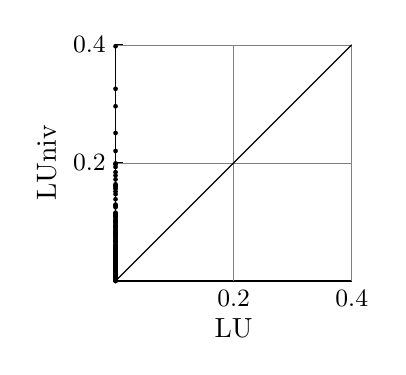
\begin{tikzpicture}

\draw (0,0) -- (3,0);
\node at (1.5,-0.6) {LU};
\node [anchor=north] at (1.5,0) {\small 0.2};
\draw (1.5,0) -- (1.5,0.1);
\draw [style=help lines] (1.5,0) -- (1.5,3);
\node [anchor=north] at (3,0) {\small 0.4};
\draw (3,0) -- (3,0.1);
\draw [style=help lines] (3,0) -- (3,3);
\draw (0,0) -- (0,3);
\node [rotate=90] at (-2.5em,1.5) {LUniv};
\node [anchor=east] at (0,1.499) {\small 0.2};
\draw (0,1.499) -- (0.1,1.499);
\draw [style=help lines] (0,1.499) -- (3,1.499);
\node [anchor=east] at (0,2.998) {\small 0.4};
\draw (0,2.998) -- (0.1,2.998);
\draw [style=help lines] (0,2.998) -- (3,2.998);
\foreach \pos in {
	(0.000000, 0.000000),
	(0.000000, 0.006027),
	(0.000000, 0.012068),
	(0.000000, 0.018078),
	(0.000000, 0.024081),
	(0.000000, 0.030102),
	(0.000000, 0.036132),
	(0.000000, 0.042135),
	(0.000000, 0.048139),
	(0.000000, 0.054173),
	(0.000000, 0.060193),
	(0.000000, 0.066204),
	(0.000000, 0.072231),
	(0.000000, 0.078267),
	(0.000000, 0.084364),
	(0.000000, 0.090399),
	(0.000000, 0.096401),
	(0.000000, 0.102428),
	(0.000000, 0.108447),
	(0.000000, 0.114679),
	(0.000000, 0.120791),
	(0.000000, 0.126880),
	(0.000000, 0.132911),
	(0.000000, 0.139104),
	(0.000000, 0.145161),
	(0.000000, 0.151976),
	(0.000000, 0.158056),
	(0.000000, 0.164294),
	(0.000000, 0.170607),
	(0.000000, 0.177083),
	(0.000000, 0.183346),
	(0.000000, 0.189531),
	(0.000000, 0.197023),
	(0.000000, 0.203202),
	(0.000000, 0.210068),
	(0.000000, 0.216346),
	(0.000000, 0.222534),
	(0.000000, 0.228814),
	(0.000000, 0.235149),
	(0.000000, 0.242236),
	(0.000000, 0.248494),
	(0.000000, 0.255682),
	(0.000000, 0.262190),
	(0.000000, 0.268595),
	(0.000000, 0.275000),
	(0.000000, 0.281250),
	(0.000000, 0.288652),
	(0.000000, 0.295468),
	(0.000000, 0.302469),
	(0.000000, 0.309633),
	(0.000000, 0.317199),
	(0.000000, 0.323920),
	(0.000000, 0.330264),
	(0.000000, 0.337955),
	(0.000000, 0.343960),
	(0.000000, 0.353213),
	(0.000000, 0.359281),
	(0.000000, 0.367948),
	(0.000000, 0.376227),
	(0.000000, 0.382883),
	(0.000000, 0.389447),
	(0.000000, 0.396635),
	(0.000000, 0.403226),
	(0.000000, 0.410584),
	(0.000000, 0.418424),
	(0.000000, 0.425226),
	(0.000000, 0.432000),
	(0.000000, 0.442446),
	(0.000000, 0.449183),
	(0.000000, 0.456933),
	(0.000000, 0.468750),
	(0.000000, 0.489614),
	(0.000000, 0.500000),
	(0.000000, 0.507201),
	(0.000000, 0.513219),
	(0.000000, 0.520112),
	(0.000000, 0.535714),
	(0.000000, 0.552826),
	(0.000000, 0.566406),
	(0.000000, 0.573940),
	(0.000000, 0.582320),
	(0.000000, 0.591603),
	(0.000000, 0.603998),
	(0.000000, 0.610329),
	(0.000000, 0.617089),
	(0.000000, 0.629845),
	(0.000000, 0.645161),
	(0.000000, 0.659843),
	(0.000000, 0.680628),
	(0.000000, 0.689189),
	(0.000000, 0.696653),
	(0.000000, 0.703125),
	(0.000000, 0.722940),
	(0.000000, 0.738137),
	(0.000000, 0.750000),
	(0.000000, 0.756961),
	(0.000000, 0.765571),
	(0.000000, 0.772382),
	(0.000000, 0.796943),
	(0.000000, 0.814917),
	(0.000000, 0.825147),
	(0.000000, 0.833333),
	(0.000000, 0.843426),
	(0.000000, 0.853716),
	(0.000000, 0.867993),
	(0.000000, 0.936396),
	(0.000000, 0.953237),
	(0.000000, 0.961538),
	(0.000000, 0.970588),
	(0.000000, 1.038405),
	(0.000000, 1.102151),
	(0.000000, 1.135487),
	(0.000000, 1.169637),
	(0.000000, 1.192255),
	(0.000000, 1.207154),
	(0.000000, 1.214489),
	(0.000000, 1.228771),
	(0.000000, 1.289409),
	(0.000000, 1.338120),
	(0.000000, 1.382175),
	(0.000000, 1.447721),
	(0.000000, 1.481127),
	(0.000000, 1.493478),
	(0.000000, 1.651376),
	(0.000000, 1.879845),
	(0.000000, 2.219101),
	(0.000000, 2.440727),
	(0.000000, 2.981462),
} \fill \pos circle(0.03);
\draw (0,0) -- (3, 3);
\end{tikzpicture}

  } \
  \subfloat[Compression ratio difference]{
    \centering
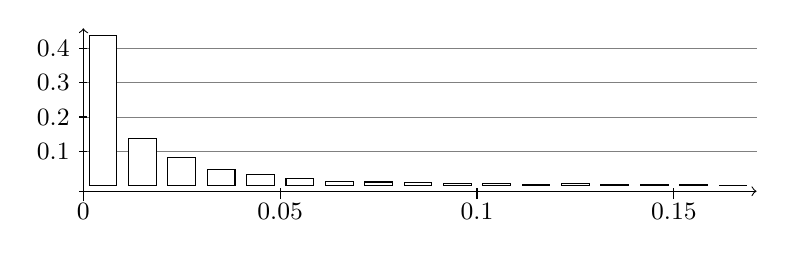
\begin{tikzpicture}
\draw[->] (-0.25,-0.2) -- (-0.25,2);
\draw [style=help lines] (-0.3,0.436406513976431) -- (8.3,0.436406513976431);
\node [anchor=east,fill=white] at (-0.3,0.436406513976431) {\small 0.1};
\draw (-0.3,0.436406513976431) -- (-0.2,0.436406513976431);
\draw [style=help lines] (-0.3,0.872813027952862) -- (8.3,0.872813027952862);
\node [anchor=east,fill=white] at (-0.3,0.872813027952862) {\small 0.2};
\draw (-0.3,0.872813027952862) -- (-0.2,0.872813027952862);
\draw [style=help lines] (-0.3,1.30921954192929) -- (8.3,1.30921954192929);
\node [anchor=east,fill=white] at (-0.3,1.30921954192929) {\small 0.3};
\draw (-0.3,1.30921954192929) -- (-0.2,1.30921954192929);
\draw [style=help lines] (-0.3,1.74562605590572) -- (8.3,1.74562605590572);
\node [anchor=east,fill=white] at (-0.3,1.74562605590572) {\small 0.4};
\draw (-0.3,1.74562605590572) -- (-0.2,1.74562605590572);
\draw[->] (-0.3,-0.07) -- (8.3,-0.07);
\node [anchor=north] at (-0.25, -0.1) {\small 0};
\draw (-0.25,-0.17) -- (-0.25,-0.03);
\node [anchor=north] at (2.25, -0.1) {\small 0.05};
\draw (2.25,-0.17) -- (2.25,-0.03);
\node [anchor=north] at (4.75, -0.1) {\small 0.1};
\draw (4.75,-0.17) -- (4.75,-0.03);
\node [anchor=north] at (7.25, -0.1) {\small 0.15};
\draw (7.25,-0.17) -- (7.25,-0.03);

\draw[fill=white] plot[ybar] coordinates {
	(6.000000, 0.027668)
	(6.500000, 0.011240)
	(7.500000, 0.014698)
	(3.000000, 0.054470)
	(5.500000, 0.014698)
	(5.000000, 0.025074)
	(8.000000, 0.005188)
	(1.500000, 0.202319)
	(4.500000, 0.032855)
	(3.500000, 0.046689)
	(0.500000, 0.601769)
	(0.000000, 1.912519)
	(4.000000, 0.044960)
	(2.500000, 0.094243)
	(1.000000, 0.361407)
	(2.000000, 0.138338)
	(7.000000, 0.012969)
};

\end{tikzpicture}
  } \
  \subfloat[Duration difference]{
    \centering
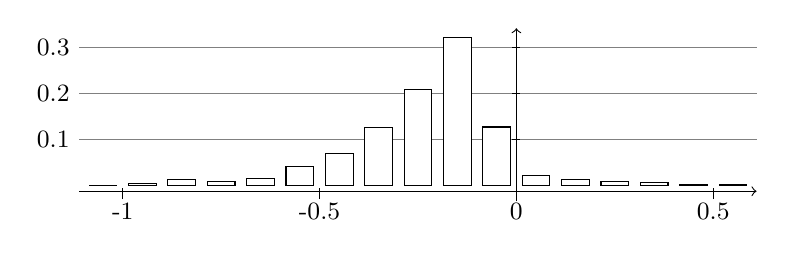
\begin{tikzpicture}
\draw[->] (-0.25,-0.2) -- (-0.25,2);
\draw [style=help lines] (-5.8,0.585829681355775) -- (2.8,0.585829681355775);
\node [anchor=east,fill=white] at (-5.8,0.585829681355775) {\small 0.1};
\draw (-0.3,0.585829681355775) -- (-0.2,0.585829681355775);
\draw [style=help lines] (-5.8,1.17165936271155) -- (2.8,1.17165936271155);
\node [anchor=east,fill=white] at (-5.8,1.17165936271155) {\small 0.2};
\draw (-0.3,1.17165936271155) -- (-0.2,1.17165936271155);
\draw [style=help lines] (-5.8,1.75748904406732) -- (2.8,1.75748904406732);
\node [anchor=east,fill=white] at (-5.8,1.75748904406732) {\small 0.3};
\draw (-0.3,1.75748904406732) -- (-0.2,1.75748904406732);
\draw[->] (-5.8,-0.07) -- (2.8,-0.07);
\node [anchor=north] at (-5.25, -0.1) {\small -1};
\draw (-5.25,-0.17) -- (-5.25,-0.03);
\node [anchor=north] at (-2.75, -0.1) {\small -0.5};
\draw (-2.75,-0.17) -- (-2.75,-0.03);
\node [anchor=north] at (-0.25, -0.1) {\small 0};
\draw (-0.25,-0.17) -- (-0.25,-0.03);
\node [anchor=north] at (2.25, -0.1) {\small 0.5};
\draw (2.25,-0.17) -- (2.25,-0.03);

\draw[fill=white] plot[ybar] coordinates {
	(1.000000, 0.048719)
	(-4.000000, 0.054519)
	(1.500000, 0.041759)
	(-4.500000, 0.077718)
	(0.000000, 0.132237)
	(-5.500000, 0.008120)
	(2.000000, 0.019720)
	(-3.500000, 0.092798)
	(0.500000, 0.080038)
	(-0.500000, 0.745862)
	(-3.000000, 0.249394)
	(-2.000000, 0.741222)
	(-1.000000, 1.882634)
	(2.500000, 0.015080)
	(-1.500000, 1.223770)
	(-5.000000, 0.025519)
	(-2.500000, 0.409470)
};

\end{tikzpicture}
  }
  \caption{Comparison between LU and LUniv}
  \label{fig:LU}
\end{figure}

\include{RPILU_charts}
\begin{figure}[tb]
  \centering
  \subfloat[Compression ratio]{
    \centering
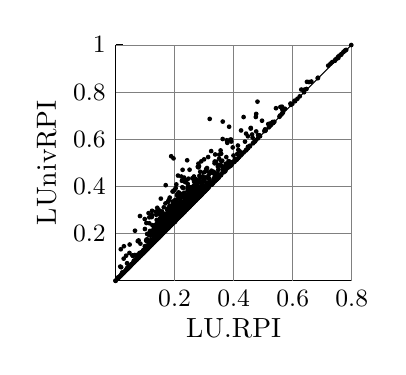
\begin{tikzpicture}

\draw (0,0) -- (3,0);
\node at (1.5,-0.6) {LU.RPI};
\node [anchor=north] at (0.75,0) {\small 0.2};
\draw (0.75,0) -- (0.75,0.1);
\draw [style=help lines] (0.75,0) -- (0.75,3);
\node [anchor=north] at (1.5,0) {\small 0.4};
\draw (1.5,0) -- (1.5,0.1);
\draw [style=help lines] (1.5,0) -- (1.5,3);
\node [anchor=north] at (2.25,0) {\small 0.6};
\draw (2.25,0) -- (2.25,0.1);
\draw [style=help lines] (2.25,0) -- (2.25,3);
\node [anchor=north] at (3,0) {\small 0.8};
\draw (3,0) -- (3,0.1);
\draw [style=help lines] (3,0) -- (3,3);
\draw (0,0) -- (0,3);
\node [rotate=90] at (-2.5em,1.5) {LUnivRPI};
\node [anchor=east] at (0,0.599) {\small 0.2};
\draw (0,0.599) -- (0.1,0.599);
\draw [style=help lines] (0,0.599) -- (3,0.599);
\node [anchor=east] at (0,1.198) {\small 0.4};
\draw (0,1.198) -- (0.1,1.198);
\draw [style=help lines] (0,1.198) -- (3,1.198);
\node [anchor=east] at (0,1.797) {\small 0.6};
\draw (0,1.797) -- (0.1,1.797);
\draw [style=help lines] (0,1.797) -- (3,1.797);
\node [anchor=east] at (0,2.396) {\small 0.8};
\draw (0,2.396) -- (0.1,2.396);
\draw [style=help lines] (0,2.396) -- (3,2.396);
\node [anchor=east] at (0,2.995) {\small 1};
\draw (0,2.995) -- (0.1,2.995);
\draw [style=help lines] (0,2.995) -- (3,2.995);
\foreach \pos in {
	(0.000000, 0.000000),
	(0.022556, 0.022556),
	(0.026866, 0.026866),
	(0.034884, 0.034884),
	(0.033771, 0.044224),
	(0.039735, 0.039735),
	(0.047782, 0.047782),
	(0.055046, 0.055046),
	(0.061529, 0.061529),
	(0.065990, 0.065990),
	(0.071429, 0.071429),
	(0.075949, 0.075949),
	(0.078947, 0.086842),
	(0.086185, 0.086185),
	(0.092593, 0.092593),
	(0.084806, 0.106007),
	(0.099919, 0.099919),
	(0.104966, 0.104966),
	(0.110092, 0.110092),
	(0.114504, 0.114504),
	(0.122041, 0.122041),
	(0.128571, 0.128571),
	(0.071303, 0.171655),
	(0.060000, 0.180000),
	(0.136364, 0.136364),
	(0.142012, 0.142012),
	(0.141340, 0.149701),
	(0.146341, 0.146341),
	(0.151899, 0.151899),
	(0.156780, 0.156780),
	(0.150729, 0.170178),
	(0.162712, 0.162712),
	(0.168000, 0.168000),
	(0.173077, 0.173077),
	(0.177515, 0.177515),
	(0.182657, 0.182657),
	(0.145941, 0.222798),
	(0.190909, 0.190909),
	(0.195918, 0.195918),
	(0.204545, 0.204545),
	(0.200856, 0.210782),
	(0.103448, 0.280788),
	(0.211973, 0.214269),
	(0.221051, 0.221549),
	(0.225348, 0.228804),
	(0.233010, 0.233010),
	(0.238054, 0.238805),
	(0.231502, 0.252513),
	(0.241615, 0.244870),
	(0.134328, 0.318408),
	(0.248121, 0.248730),
	(0.242163, 0.256984),
	(0.252074, 0.257542),
	(0.258219, 0.258427),
	(0.252366, 0.264420),
	(0.259315, 0.265075),
	(0.265513, 0.265513),
	(0.269674, 0.269879),
	(0.222026, 0.314537),
	(0.268906, 0.276229),
	(0.214286, 0.321429),
	(0.275511, 0.275726),
	(0.270148, 0.283768),
	(0.176471, 0.352941),
	(0.279610, 0.281561),
	(0.066667, 0.400000),
	(0.286393, 0.287182),
	(0.244898, 0.326531),
	(0.285177, 0.295294),
	(0.291667, 0.291667),
	(0.296928, 0.296928),
	(0.300130, 0.302734),
	(0.307058, 0.307831),
	(0.302600, 0.313489),
	(0.284211, 0.331579),
	(0.301693, 0.320207),
	(0.311584, 0.311792),
	(0.310383, 0.317737),
	(0.316484, 0.316484),
	(0.106195, 0.438053),
	(0.313074, 0.324653),
	(0.320626, 0.322031),
	(0.325434, 0.326011),
	(0.318974, 0.334808),
	(0.315469, 0.341907),
	(0.326271, 0.332227),
	(0.305505, 0.353670),
	(0.332547, 0.332547),
	(0.324825, 0.343055),
	(0.334427, 0.339516),
	(0.333588, 0.346735),
	(0.340909, 0.340909),
	(0.329980, 0.357339),
	(0.339402, 0.348831),
	(0.345455, 0.345455),
	(0.332109, 0.364030),
	(0.179221, 0.459740),
	(0.345945, 0.353188),
	(0.351792, 0.351792),
	(0.348837, 0.358804),
	(0.356265, 0.356512),
	(0.355974, 0.364317),
	(0.360921, 0.360921),
	(0.346738, 0.375993),
	(0.366084, 0.366105),
	(0.361655, 0.370806),
	(0.360262, 0.377479),
	(0.370662, 0.370684),
	(0.367135, 0.378819),
	(0.355440, 0.392429),
	(0.364115, 0.385163),
	(0.374950, 0.374988),
	(0.372969, 0.382027),
	(0.379331, 0.379521),
	(0.369434, 0.391811),
	(0.376535, 0.388813),
	(0.383470, 0.384334),
	(0.381187, 0.393701),
	(0.388263, 0.388556),
	(0.381963, 0.401857),
	(0.392587, 0.392718),
	(0.389875, 0.398283),
	(0.388031, 0.404186),
	(0.396528, 0.397336),
	(0.380041, 0.416875),
	(0.395580, 0.403315),
	(0.315881, 0.471023),
	(0.401438, 0.401541),
	(0.391266, 0.417037),
	(0.400591, 0.410781),
	(0.405797, 0.405797),
	(0.371866, 0.438719),
	(0.282110, 0.502294),
	(0.393529, 0.422730),
	(0.405007, 0.414862),
	(0.410853, 0.410853),
	(0.399240, 0.424905),
	(0.392027, 0.433555),
	(0.405433, 0.422848),
	(0.412802, 0.417751),
	(0.292683, 0.512195),
	(0.402659, 0.435226),
	(0.419692, 0.419692),
	(0.421184, 0.425797),
	(0.427612, 0.427734),
	(0.423215, 0.435209),
	(0.415609, 0.443377),
	(0.429151, 0.434300),
	(0.423256, 0.445349),
	(0.435256, 0.435368),
	(0.432916, 0.441732),
	(0.424676, 0.454307),
	(0.439511, 0.441052),
	(0.430712, 0.453184),
	(0.439107, 0.449259),
	(0.444795, 0.444795),
	(0.426309, 0.467243),
	(0.447369, 0.450247),
	(0.440077, 0.458763),
	(0.435583, 0.463190),
	(0.397732, 0.498631),
	(0.451080, 0.455735),
	(0.445668, 0.461316),
	(0.389262, 0.510067),
	(0.457061, 0.457419),
	(0.434292, 0.480493),
	(0.451189, 0.467641),
	(0.442037, 0.476676),
	(0.456647, 0.463621),
	(0.462555, 0.462555),
	(0.393516, 0.523691),
	(0.430969, 0.496568),
	(0.453807, 0.478173),
	(0.463568, 0.469922),
	(0.459797, 0.476456),
	(0.407631, 0.524096),
	(0.469785, 0.470615),
	(0.454803, 0.488338),
	(0.473595, 0.475379),
	(0.468025, 0.481294),
	(0.458019, 0.495482),
	(0.478819, 0.478960),
	(0.466975, 0.490559),
	(0.247059, 0.635294),
	(0.476424, 0.489682),
	(0.482688, 0.483707),
	(0.449591, 0.514986),
	(0.462162, 0.510811),
	(0.484317, 0.490023),
	(0.469266, 0.506422),
	(0.476190, 0.503401),
	(0.483945, 0.496157),
	(0.490444, 0.491278),
	(0.491765, 0.497793),
	(0.483823, 0.510249),
	(0.497727, 0.498605),
	(0.481799, 0.517131),
	(0.473310, 0.528146),
	(0.491691, 0.512664),
	(0.502547, 0.502744),
	(0.497695, 0.509062),
	(0.492667, 0.520186),
	(0.503893, 0.509530),
	(0.401709, 0.593831),
	(0.500591, 0.516054),
	(0.421813, 0.583443),
	(0.492559, 0.526590),
	(0.498788, 0.522055),
	(0.509770, 0.511427),
	(0.441951, 0.573659),
	(0.505588, 0.520140),
	(0.496173, 0.531888),
	(0.485763, 0.542180),
	(0.514151, 0.516221),
	(0.502830, 0.528835),
	(0.417722, 0.600000),
	(0.497124, 0.539432),
	(0.511285, 0.526364),
	(0.519434, 0.519518),
	(0.509844, 0.532426),
	(0.505670, 0.536929),
	(0.521818, 0.525696),
	(0.500000, 0.547297),
	(0.516432, 0.533646),
	(0.523554, 0.531853),
	(0.529006, 0.529195),
	(0.520112, 0.541093),
	(0.510104, 0.552888),
	(0.479666, 0.579944),
	(0.525795, 0.538924),
	(0.530846, 0.535292),
	(0.373010, 0.657316),
	(0.536817, 0.536817),
	(0.529679, 0.544022),
	(0.522862, 0.550834),
	(0.464343, 0.607429),
	(0.529143, 0.552029),
	(0.540770, 0.541800),
	(0.537037, 0.549383),
	(0.439024, 0.633208),
	(0.517061, 0.572528),
	(0.529363, 0.561219),
	(0.545306, 0.545851),
	(0.542941, 0.551788),
	(0.539863, 0.559226),
	(0.549707, 0.550018),
	(0.537190, 0.566116),
	(0.529698, 0.573515),
	(0.518506, 0.584720),
	(0.547740, 0.557584),
	(0.554702, 0.554702),
	(0.544983, 0.564446),
	(0.536177, 0.575181),
	(0.470004, 0.631404),
	(0.520354, 0.593363),
	(0.550684, 0.566530),
	(0.557879, 0.560014),
	(0.488646, 0.622150),
	(0.545502, 0.574295),
	(0.557056, 0.569210),
	(0.563150, 0.563276),
	(0.550360, 0.578237),
	(0.534542, 0.593023),
	(0.528352, 0.602062),
	(0.564607, 0.569443),
	(0.493103, 0.636782),
	(0.501548, 0.631579),
	(0.570848, 0.571033),
	(0.555000, 0.587857),
	(0.559933, 0.583657),
	(0.565851, 0.578345),
	(0.540089, 0.607969),
	(0.574954, 0.575646),
	(0.556161, 0.595420),
	(0.568569, 0.585179),
	(0.549451, 0.604396),
	(0.578765, 0.580405),
	(0.484605, 0.662651),
	(0.563822, 0.598104),
	(0.523636, 0.635455),
	(0.535851, 0.625717),
	(0.576655, 0.588464),
	(0.561896, 0.604462),
	(0.584743, 0.584743),
	(0.576630, 0.595498),
	(0.559254, 0.613182),
	(0.568398, 0.604883),
	(0.548929, 0.623625),
	(0.391560, 0.733072),
	(0.584871, 0.591158),
	(0.575703, 0.603696),
	(0.507763, 0.662100),
	(0.585389, 0.597674),
	(0.591887, 0.592359),
	(0.578804, 0.611413),
	(0.587723, 0.603244),
	(0.594961, 0.597991),
	(0.576445, 0.617501),
	(0.546099, 0.645390),
	(0.586176, 0.609515),
	(0.429007, 0.729997),
	(0.468547, 0.706074),
	(0.594006, 0.606043),
	(0.572968, 0.626644),
	(0.599106, 0.602735),
	(0.564000, 0.636000),
	(0.570608, 0.634647),
	(0.585509, 0.622715),
	(0.598271, 0.610833),
	(0.545997, 0.659373),
	(0.604267, 0.606442),
	(0.581081, 0.632883),
	(0.573620, 0.640412),
	(0.565923, 0.648073),
	(0.597603, 0.619472),
	(0.587071, 0.630607),
	(0.603268, 0.615260),
	(0.592888, 0.626505),
	(0.609664, 0.610784),
	(0.556808, 0.660885),
	(0.582822, 0.639264),
	(0.599952, 0.624997),
	(0.573326, 0.649538),
	(0.370787, 0.783708),
	(0.609045, 0.617268),
	(0.590614, 0.636554),
	(0.508787, 0.703866),
	(0.566809, 0.658723),
	(0.546019, 0.676319),
	(0.615541, 0.616339),
	(0.576191, 0.655027),
	(0.600816, 0.632653),
	(0.609176, 0.625043),
	(0.562297, 0.669556),
	(0.585000, 0.650000),
	(0.509510, 0.711224),
	(0.593318, 0.644098),
	(0.615639, 0.622825),
	(0.542510, 0.688259),
	(0.310345, 0.821839),
	(0.614063, 0.629464),
	(0.621995, 0.622704),
	(0.564644, 0.675462),
	(0.611009, 0.638532),
	(0.604077, 0.647931),
	(0.620371, 0.632567),
	(0.589699, 0.661359),
	(0.625328, 0.628383),
	(0.556856, 0.689799),
	(0.578740, 0.671915),
	(0.533173, 0.709522),
	(0.617043, 0.638604),
	(0.600000, 0.660502),
	(0.626232, 0.637315),
	(0.632022, 0.632748),
	(0.524272, 0.724919),
	(0.591534, 0.673016),
	(0.600467, 0.668638),
	(0.622877, 0.648033),
	(0.628127, 0.643134),
	(0.634298, 0.638813),
	(0.615904, 0.658767),
	(0.600000, 0.675000),
	(0.606099, 0.670902),
	(0.640281, 0.640691),
	(0.634599, 0.646769),
	(0.628846, 0.653159),
	(0.624590, 0.657787),
	(0.568508, 0.707735),
	(0.580034, 0.700516),
	(0.586466, 0.696026),
	(0.619637, 0.666933),
	(0.612762, 0.673381),
	(0.641038, 0.647636),
	(0.636210, 0.652868),
	(0.428571, 0.805132),
	(0.604142, 0.685584),
	(0.628272, 0.665766),
	(0.621106, 0.673367),
	(0.642096, 0.654123),
	(0.646739, 0.649954),
	(0.614955, 0.680804),
	(0.564516, 0.725806),
	(0.637981, 0.664236),
	(0.622199, 0.681605),
	(0.650591, 0.654940),
	(0.604580, 0.698931),
	(0.585600, 0.715200),
	(0.646423, 0.661398),
	(0.610417, 0.695833),
	(0.629728, 0.679275),
	(0.637287, 0.672988),
	(0.581315, 0.722491),
	(0.450673, 0.810538),
	(0.644534, 0.669809),
	(0.656579, 0.658198),
	(0.652430, 0.662739),
	(0.577845, 0.730080),
	(0.608434, 0.704819),
	(0.460317, 0.809524),
	(0.522321, 0.772321),
	(0.624582, 0.692308),
	(0.637964, 0.680780),
	(0.631579, 0.687673),
	(0.560786, 0.747258),
	(0.643736, 0.677870),
	(0.593318, 0.722940),
	(0.653666, 0.669501),
	(0.661269, 0.662350),
	(0.649566, 0.674162),
	(0.574523, 0.740901),
	(0.660618, 0.668743),
	(0.643099, 0.685972),
	(0.656688, 0.674930),
	(0.649706, 0.683872),
	(0.666667, 0.668519),
	(0.605181, 0.725275),
	(0.622695, 0.710511),
	(0.591488, 0.737723),
	(0.663555, 0.674274),
	(0.637902, 0.699662),
	(0.643500, 0.696750),
	(0.617747, 0.720137),
	(0.649499, 0.691887),
	(0.656291, 0.685489),
	(0.671732, 0.671791),
	(0.669326, 0.677714),
	(0.631854, 0.712794),
	(0.613890, 0.730467),
	(0.462527, 0.835118),
	(0.666184, 0.684095),
	(0.419355, 0.858871),
	(0.660603, 0.690761),
	(0.675292, 0.676972),
	(0.628440, 0.723394),
	(0.643590, 0.710876),
	(0.672229, 0.684224),
	(0.653345, 0.702867),
	(0.622140, 0.731121),
	(0.668372, 0.690233),
	(0.660365, 0.699210),
	(0.680638, 0.680638),
	(0.651363, 0.709355),
	(0.667491, 0.696490),
	(0.676734, 0.688607),
	(0.619124, 0.741036),
	(0.579987, 0.772154),
	(0.561447, 0.786026),
	(0.673967, 0.694356),
	(0.663454, 0.705653),
	(0.682847, 0.688796),
	(0.660585, 0.711498),
	(0.670562, 0.703433),
	(0.641260, 0.730488),
	(0.680286, 0.695778),
	(0.628086, 0.745474),
	(0.688761, 0.689821),
	(0.670355, 0.710638),
	(0.677700, 0.704518),
	(0.663000, 0.718500),
	(0.685052, 0.701381),
	(0.691047, 0.695599),
	(0.656683, 0.728404),
	(0.676932, 0.711125),
	(0.670711, 0.717269),
	(0.516673, 0.837669),
	(0.684158, 0.707921),
	(0.632212, 0.754808),
	(0.666667, 0.725074),
	(0.655629, 0.735099),
	(0.690789, 0.703205),
	(0.696795, 0.697788),
	(0.585000, 0.795000),
	(0.601744, 0.784884),
	(0.698192, 0.704061),
	(0.687540, 0.715279),
	(0.677248, 0.725085),
	(0.595916, 0.794554),
	(0.647197, 0.753742),
	(0.661702, 0.741162),
	(0.695178, 0.711721),
	(0.685511, 0.722587),
	(0.634398, 0.768280),
	(0.639537, 0.764626),
	(0.701914, 0.709410),
	(0.692243, 0.721331),
	(0.672467, 0.740020),
	(0.617111, 0.788219),
	(0.667333, 0.746549),
	(0.707872, 0.708476),
	(0.679007, 0.736222),
	(0.688236, 0.728005),
	(0.463520, 0.888185),
	(0.684329, 0.732824),
	(0.698323, 0.720509),
	(0.703722, 0.716146),
	(0.655558, 0.763165),
	(0.612200, 0.799564),
	(0.569992, 0.830378),
	(0.710780, 0.715610),
	(0.693350, 0.732871),
	(0.704622, 0.722703),
	(0.666290, 0.759828),
	(0.673236, 0.755245),
	(0.648719, 0.776775),
	(0.703671, 0.729185),
	(0.712065, 0.722339),
	(0.697936, 0.737336),
	(0.510245, 0.877917),
	(0.679634, 0.755835),
	(0.718264, 0.719546),
	(0.688536, 0.748468),
	(0.541907, 0.862479),
	(0.711564, 0.729999),
	(0.666401, 0.771497),
	(0.706723, 0.735310),
	(0.717212, 0.726716),
	(0.697500, 0.747500),
	(0.662409, 0.779562),
	(0.704826, 0.741900),
	(0.693477, 0.753305),
	(0.713230, 0.736576),
	(0.723319, 0.728187),
	(0.646501, 0.798561),
	(0.653531, 0.793416),
	(0.719399, 0.734431),
	(0.636953, 0.807131),
	(0.668405, 0.782414),
	(0.705277, 0.749387),
	(0.700897, 0.754709),
	(0.679426, 0.775120),
	(0.692854, 0.763916),
	(0.729127, 0.729710),
	(0.605948, 0.837361),
	(0.726049, 0.735930),
	(0.719982, 0.742152),
	(0.711864, 0.750934),
	(0.661538, 0.796154),
	(0.689420, 0.773281),
	(0.701099, 0.762805),
	(0.654944, 0.805242),
	(0.634301, 0.822142),
	(0.719828, 0.748922),
	(0.732082, 0.737305),
	(0.710153, 0.759074),
	(0.695481, 0.772543),
	(0.725632, 0.744585),
	(0.676320, 0.790689),
	(0.715920, 0.756168),
	(0.685349, 0.786651),
	(0.733915, 0.743184),
	(0.730391, 0.748385),
	(0.667355, 0.806026),
	(0.589641, 0.864542),
	(0.723855, 0.756664),
	(0.714837, 0.765194),
	(0.677005, 0.799572),
	(0.569826, 0.879440),
	(0.741053, 0.742176),
	(0.698537, 0.782439),
	(0.737185, 0.749359),
	(0.730241, 0.756586),
	(0.713836, 0.772537),
	(0.722222, 0.766667),
	(0.691682, 0.795848),
	(0.745814, 0.746014),
	(0.736735, 0.755685),
	(0.545735, 0.903392),
	(0.712220, 0.779365),
	(0.731443, 0.764387),
	(0.719450, 0.775787),
	(0.628713, 0.851485),
	(0.752504, 0.745351),
	(0.658188, 0.829889),
	(0.653114, 0.833901),
	(0.589286, 0.880309),
	(0.745298, 0.753858),
	(0.740913, 0.760485),
	(0.727334, 0.773932),
	(0.717965, 0.783791),
	(0.684952, 0.813128),
	(0.677342, 0.821457),
	(0.737080, 0.769073),
	(0.752855, 0.754345),
	(0.747506, 0.762013),
	(0.529625, 0.926844),
	(0.742829, 0.767214),
	(0.731650, 0.779006),
	(0.716727, 0.793385),
	(0.700855, 0.809117),
	(0.695017, 0.815046),
	(0.755359, 0.760519),
	(0.748395, 0.769489),
	(0.682175, 0.829587),
	(0.727246, 0.790754),
	(0.720415, 0.798157),
	(0.732510, 0.787380),
	(0.695531, 0.821229),
	(0.761719, 0.761719),
	(0.743410, 0.780264),
	(0.755990, 0.768397),
	(0.749288, 0.776353),
	(0.716005, 0.808208),
	(0.689072, 0.832689),
	(0.679669, 0.840574),
	(0.712500, 0.813281),
	(0.701964, 0.822508),
	(0.763443, 0.767710),
	(0.663889, 0.855556),
	(0.745673, 0.787058),
	(0.759090, 0.774591),
	(0.730271, 0.803116),
	(0.719383, 0.814065),
	(0.755293, 0.781614),
	(0.716692, 0.820061),
	(0.770690, 0.770690),
	(0.765752, 0.776330),
	(0.750000, 0.792339),
	(0.761941, 0.781766),
	(0.711746, 0.828203),
	(0.743503, 0.800000),
	(0.736919, 0.807776),
	(0.690962, 0.847522),
	(0.759612, 0.787573),
	(0.703877, 0.838235),
	(0.752134, 0.797977),
	(0.768352, 0.782423),
	(0.680707, 0.860054),
	(0.773592, 0.777800),
	(0.712261, 0.836311),
	(0.766092, 0.788252),
	(0.719057, 0.834971),
	(0.775215, 0.783655),
	(0.760090, 0.798694),
	(0.740310, 0.817829),
	(0.756032, 0.804290),
	(0.748544, 0.812621),
	(0.771443, 0.791078),
	(0.766607, 0.797149),
	(0.781686, 0.783581),
	(0.746939, 0.818878),
	(0.765415, 0.803234),
	(0.777372, 0.792492),
	(0.755097, 0.813846),
	(0.773864, 0.797727),
	(0.785974, 0.788430),
	(0.655539, 0.901366),
	(0.745161, 0.830323),
	(0.612552, 0.932528),
	(0.752003, 0.824387),
	(0.667042, 0.895388),
	(0.781806, 0.798802),
	(0.673901, 0.892324),
	(0.769280, 0.812123),
	(0.762641, 0.819098),
	(0.776916, 0.806429),
	(0.788243, 0.796459),
	(0.783488, 0.804971),
	(0.740307, 0.845244),
	(0.686636, 0.889401),
	(0.776081, 0.812621),
	(0.760320, 0.827950),
	(0.723902, 0.860251),
	(0.676281, 0.898292),
	(0.752446, 0.836413),
	(0.736522, 0.851304),
	(0.769320, 0.822581),
	(0.793541, 0.799485),
	(0.758538, 0.834783),
	(0.782743, 0.812492),
	(0.789756, 0.805837),
	(0.766946, 0.828452),
	(0.743195, 0.851251),
	(0.729794, 0.864105),
	(0.685665, 0.899827),
	(0.756303, 0.842174),
	(0.779279, 0.821922),
	(0.797406, 0.804794),
	(0.665476, 0.917857),
	(0.788634, 0.814670),
	(0.726562, 0.870536),
	(0.720643, 0.876391),
	(0.766905, 0.836463),
	(0.771681, 0.832610),
	(0.739572, 0.861497),
	(0.672671, 0.914907),
	(0.747226, 0.856350),
	(0.803742, 0.803906),
	(0.796925, 0.811321),
	(0.781915, 0.828191),
	(0.718127, 0.885516),
	(0.795444, 0.817599),
	(0.726901, 0.880551),
	(0.790971, 0.824062),
	(0.805315, 0.810602),
	(0.768365, 0.845797),
	(0.685448, 0.914622),
	(0.783784, 0.834719),
	(0.734115, 0.879349),
	(0.803759, 0.816661),
	(0.760829, 0.858571),
	(0.790482, 0.832145),
	(0.685934, 0.921002),
	(0.797017, 0.826848),
	(0.742698, 0.876596),
	(0.810193, 0.815343),
	(0.778365, 0.848306),
	(0.807780, 0.821442),
	(0.789641, 0.839030),
	(0.770155, 0.857259),
	(0.798701, 0.833079),
	(0.805171, 0.828255),
	(0.737643, 0.889734),
	(0.817518, 0.817518),
	(0.795068, 0.841959),
	(0.811087, 0.826661),
	(0.788985, 0.849370),
	(0.776724, 0.861318),
	(0.817366, 0.823863),
	(0.785443, 0.854699),
	(0.807268, 0.834232),
	(0.758602, 0.879847),
	(0.771593, 0.870304),
	(0.803714, 0.841228),
	(0.740764, 0.897828),
	(0.797900, 0.848644),
	(0.718232, 0.917127),
	(0.823412, 0.825324),
	(0.813662, 0.835982),
	(0.819174, 0.831425),
	(0.633627, 0.982356),
	(0.685069, 0.948557),
	(0.803307, 0.851416),
	(0.797526, 0.858014),
	(0.793062, 0.863475),
	(0.828531, 0.829556),
	(0.762326, 0.891277),
	(0.820397, 0.838164),
	(0.784149, 0.873711),
	(0.812191, 0.847948),
	(0.736986, 0.915068),
	(0.826704, 0.836351),
	(0.802029, 0.862078),
	(0.820010, 0.846003),
	(0.792307, 0.872060),
	(0.833333, 0.833333),
	(0.726841, 0.928741),
	(0.797967, 0.868617),
	(0.811892, 0.855863),
	(0.785081, 0.880543),
	(0.754135, 0.907903),
	(0.819079, 0.852418),
	(0.767694, 0.899439),
	(0.832350, 0.840080),
	(0.828667, 0.846053),
	(0.837987, 0.837987),
	(0.782983, 0.890057),
	(0.792653, 0.881616),
	(0.826393, 0.852409),
	(0.819486, 0.860825),
	(0.727067, 0.940430),
	(0.836393, 0.845172),
	(0.575385, 1.043077),
	(0.832663, 0.851971),
	(0.807692, 0.876244),
	(0.722054, 0.948640),
	(0.843263, 0.844408),
	(0.817591, 0.869343),
	(0.829926, 0.859287),
	(0.781863, 0.904638),
	(0.800730, 0.889980),
	(0.837404, 0.856306),
	(0.826198, 0.868371),
	(0.759116, 0.928177),
	(0.847135, 0.849730),
	(0.800099, 0.896229),
	(0.835699, 0.863656),
	(0.666786, 1.000718),
	(0.844348, 0.857575),
	(0.809672, 0.891120),
	(0.852272, 0.853398),
	(0.830852, 0.875744),
	(0.837015, 0.870148),
	(0.816016, 0.890139),
	(0.666833, 1.008492),
	(0.852095, 0.860172),
	(0.844291, 0.868977),
	(0.815109, 0.896543),
	(0.771299, 0.936416),
	(0.738592, 0.963380),
	(0.790733, 0.922902),
	(0.835438, 0.882891),
	(0.726354, 0.974640),
	(0.859717, 0.859949),
	(0.852205, 0.867867),
	(0.825727, 0.893621),
	(0.844675, 0.875801),
	(0.830769, 0.889718),
	(0.814206, 0.905047),
	(0.756522, 0.954037),
	(0.826138, 0.899650),
	(0.859010, 0.869109),
	(0.864238, 0.864238),
	(0.850903, 0.877384),
	(0.846560, 0.883142),
	(0.753233, 0.964170),
	(0.839432, 0.891089),
	(0.835474, 0.896715),
	(0.789634, 0.939024),
	(0.738386, 0.980440),
	(0.856913, 0.878858),
	(0.867594, 0.869941),
	(0.862375, 0.875694),
	(0.808989, 0.926966),
	(0.766491, 0.962527),
	(0.800960, 0.935654),
	(0.855366, 0.887494),
	(0.679567, 1.028742),
	(0.843976, 0.898945),
	(0.835995, 0.906514),
	(0.823688, 0.918945),
	(0.869136, 0.876543),
	(0.832595, 0.911866),
	(0.852615, 0.894966),
	(0.864639, 0.885630),
	(0.876246, 0.876246),
	(0.833703, 0.917823),
	(0.726064, 1.005319),
	(0.773781, 0.969881),
	(0.858359, 0.898429),
	(0.742748, 0.997710),
	(0.864124, 0.895171),
	(0.845124, 0.913660),
	(0.854105, 0.907023),
	(0.876621, 0.885399),
	(0.779549, 0.973081),
	(0.882249, 0.882544),
	(0.774444, 0.979307),
	(0.815476, 0.946429),
	(0.864307, 0.902655),
	(0.822434, 0.941317),
	(0.808412, 0.953735),
	(0.799927, 0.962326),
	(0.878003, 0.893095),
	(0.833107, 0.936228),
	(0.859507, 0.912824),
	(0.884972, 0.888653),
	(0.872123, 0.904038),
	(0.867658, 0.908618),
	(0.814205, 0.957124),
	(0.825133, 0.948319),
	(0.882709, 0.897326),
	(0.848735, 0.931793),
	(0.888543, 0.894672),
	(0.688679, 1.056604),
	(0.867640, 0.915815),
	(0.832285, 0.949161),
	(0.877278, 0.910308),
	(0.826817, 0.956864),
	(0.888577, 0.900904),
	(0.846510, 0.940787),
	(0.796236, 0.986088),
	(0.886070, 0.907241),
	(0.874576, 0.918644),
	(0.754720, 1.020875),
	(0.897022, 0.898883),
	(0.867135, 0.927823),
	(0.882597, 0.914685),
	(0.837828, 0.959913),
	(0.894769, 0.907158),
	(0.825176, 0.971622),
	(0.857028, 0.944177),
	(0.863116, 0.938974),
	(0.901963, 0.902349),
	(0.881197, 0.922652),
	(0.876364, 0.927879),
	(0.888043, 0.918335),
	(0.759825, 1.027293),
	(0.894570, 0.914723),
	(0.849595, 0.958964),
	(0.772702, 1.022014),
	(0.873278, 0.937611),
	(0.886649, 0.926162),
	(0.813071, 0.991831),
	(0.864382, 0.948359),
	(0.902947, 0.911879),
	(0.896050, 0.920891),
	(0.861226, 0.953706),
	(0.880961, 0.936162),
	(0.876522, 0.943602),
	(0.830447, 0.984751),
	(0.909155, 0.913760),
	(0.887076, 0.935626),
	(0.904283, 0.919380),
	(0.859554, 0.961979),
	(0.869005, 0.954263),
	(0.902157, 0.925133),
	(0.899661, 0.932021),
	(0.912559, 0.919806),
	(0.881214, 0.951996),
	(0.821842, 1.003702),
	(0.906635, 0.930711),
	(0.889027, 0.948878),
	(0.878439, 0.959754),
	(0.920522, 0.920681),
	(0.895837, 0.945412),
	(0.912844, 0.930275),
	(0.865385, 0.975962),
	(0.905430, 0.940045),
	(0.918696, 0.927155),
	(0.875087, 0.969209),
	(0.912332, 0.937432),
	(0.895696, 0.954846),
	(0.886838, 0.963884),
	(0.842135, 1.005741),
	(0.922233, 0.934270),
	(0.927792, 0.928813),
	(0.852545, 0.998402),
	(0.910633, 0.946380),
	(0.879971, 0.975192),
	(0.907781, 0.952450),
	(0.918374, 0.944151),
	(0.879410, 0.981398),
	(0.900402, 0.964716),
	(0.925898, 0.941940),
	(0.917570, 0.950108),
	(0.888685, 0.977303),
	(0.798165, 1.052752),
	(0.867351, 0.997069),
	(0.816955, 1.039100),
	(0.913379, 0.955772),
	(0.898831, 0.971903),
	(0.936548, 0.936548),
	(0.924197, 0.949036),
	(0.908441, 0.964235),
	(0.934385, 0.946950),
	(0.939553, 0.941974),
	(0.903131, 0.977129),
	(0.927783, 0.954009),
	(0.921659, 0.961598),
	(0.913119, 0.970043),
	(0.825320, 1.046414),
	(0.884778, 1.000000),
	(0.782450, 1.084095),
	(0.934835, 0.955828),
	(0.912584, 0.977324),
	(0.890380, 0.997763),
	(0.930026, 0.961872),
	(0.906975, 0.984004),
	(0.876581, 1.011339),
	(0.947368, 0.947368),
	(0.942578, 0.954650),
	(0.929099, 0.967955),
	(0.899836, 0.996716),
	(0.890168, 1.007218),
	(0.724341, 1.133580),
	(0.922958, 0.980740),
	(0.928636, 0.975610),
	(0.949709, 0.955678),
	(0.944774, 0.960749),
	(0.917946, 0.987524),
	(0.911232, 0.993890),
	(0.936704, 0.970726),
	(0.732907, 1.135946),
	(0.895477, 1.012931),
	(0.942718, 0.969903),
	(0.785941, 1.102574),
	(0.952672, 0.963724),
	(0.940425, 0.976972),
	(0.904242, 1.010667),
	(0.948772, 0.969991),
	(0.933962, 0.986097),
	(0.961965, 0.961980),
	(0.918182, 1.006061),
	(0.927236, 0.998131),
	(0.912423, 1.012113),
	(0.947030, 0.980202),
	(0.960529, 0.967888),
	(0.884828, 1.037824),
	(0.853345, 1.064688),
	(0.936433, 0.993359),
	(0.942857, 0.989204),
	(0.860868, 1.062904),
	(0.961832, 0.976251),
	(0.892528, 1.040590),
	(0.637209, 1.213953),
	(0.931275, 1.007495),
	(0.939717, 1.000775),
	(0.967768, 0.973737),
	(0.950923, 0.990199),
	(0.960726, 0.982880),
	(0.947215, 0.996108),
	(0.822586, 1.101931),
	(0.749035, 1.154440),
	(0.924212, 1.021872),
	(0.905206, 1.039677),
	(0.820612, 1.107710),
	(0.969894, 0.979735),
	(0.800135, 1.122916),
	(0.940496, 1.009096),
	(0.975877, 0.975877),
	(0.954348, 0.997205),
	(0.948519, 1.003469),
	(0.963449, 0.989462),
	(0.973752, 0.985375),
	(0.958177, 1.002289),
	(0.921896, 1.039591),
	(0.939249, 1.025460),
	(0.954390, 1.012324),
	(0.964705, 1.002667),
	(0.865155, 1.090229),
	(0.972208, 0.997640),
	(0.910922, 1.054497),
	(0.961789, 1.008388),
	(0.979878, 0.993917),
	(0.955010, 1.019264),
	(0.941893, 1.031733),
	(0.969964, 1.006613),
	(0.987623, 0.990340),
	(0.933549, 1.042139),
	(0.896766, 1.074251),
	(0.918512, 1.058189),
	(0.981826, 1.000606),
	(0.955192, 1.026282),
	(0.763975, 1.177019),
	(0.990070, 0.997471),
	(0.966117, 1.021978),
	(0.980049, 1.008943),
	(0.954873, 1.033354),
	(0.940157, 1.047469),
	(0.996301, 0.996521),
	(0.907174, 1.079490),
	(0.987425, 1.007186),
	(0.876276, 1.106824),
	(0.966133, 1.029369),
	(0.939538, 1.054509),
	(0.979372, 1.020269),
	(0.893339, 1.096430),
	(0.993639, 1.009404),
	(0.998823, 1.004474),
	(0.871249, 1.117377),
	(0.969437, 1.039258),
	(0.941806, 1.065429),
	(0.993137, 1.018531),
	(0.986210, 1.025451),
	(1.003945, 1.009864),
	(0.920327, 1.087845),
	(1.000000, 1.015802),
	(0.978042, 1.039373),
	(0.960915, 1.055291),
	(0.988661, 1.032756),
	(1.001526, 1.022121),
	(0.952574, 1.068690),
	(1.008472, 1.017123),
	(0.929279, 1.090523),
	(0.986883, 1.040895),
	(0.996390, 1.032315),
	(1.016323, 1.016323),
	(0.964615, 1.066333),
	(0.975044, 1.059489),
	(0.997587, 1.039535),
	(1.011883, 1.030027),
	(1.020385, 1.023039),
	(1.005682, 1.037642),
	(0.960963, 1.080101),
	(0.978354, 1.065608),
	(0.772277, 1.223762),
	(0.973790, 1.070565),
	(1.020000, 1.030410),
	(0.986317, 1.064894),
	(0.999707, 1.052855),
	(0.966887, 1.086093),
	(1.028347, 1.029936),
	(1.020624, 1.037675),
	(0.859021, 1.177577),
	(1.018635, 1.043574),
	(0.848035, 1.187249),
	(0.998120, 1.065789),
	(1.015409, 1.049522),
	(0.930401, 1.125835),
	(0.965839, 1.096273),
	(1.009126, 1.057831),
	(1.031003, 1.036613),
	(1.028920, 1.042840),
	(0.992857, 1.078125),
	(1.008931, 1.064095),
	(0.915758, 1.149091),
	(0.990734, 1.086082),
	(0.963624, 1.115992),
	(1.030576, 1.056355),
	(0.980676, 1.103060),
	(1.021932, 1.065716),
	(1.037180, 1.052632),
	(0.999277, 1.090318),
	(1.029287, 1.062539),
	(0.945290, 1.140140),
	(1.047563, 1.047563),
	(1.040267, 1.058905),
	(1.037140, 1.065187),
	(0.957038, 1.138026),
	(1.002990, 1.100149),
	(0.991470, 1.110630),
	(1.047209, 1.058666),
	(1.026612, 1.078813),
	(0.913861, 1.176977),
	(1.032982, 1.074318),
	(1.045973, 1.065022),
	(0.980392, 1.127451),
	(0.939932, 1.163140),
	(1.051795, 1.066769),
	(1.047029, 1.072768),
	(1.060007, 1.060903),
	(1.038868, 1.088425),
	(0.955121, 1.162619),
	(1.047020, 1.080795),
	(1.064417, 1.065936),
	(1.053088, 1.077463),
	(1.023993, 1.105250),
	(1.007869, 1.120984),
	(1.065738, 1.072539),
	(0.922700, 1.198694),
	(1.061715, 1.077692),
	(1.018042, 1.119386),
	(1.030645, 1.108065),
	(1.072314, 1.072422),
	(0.941620, 1.189381),
	(1.052946, 1.092229),
	(1.042504, 1.103676),
	(1.060264, 1.087171),
	(0.960531, 1.177127),
	(1.051619, 1.099190),
	(1.067385, 1.084906),
	(0.843373, 1.269076),
	(1.046053, 1.108553),
	(1.074934, 1.083641),
	(1.043822, 1.115331),
	(1.080665, 1.080901),
	(1.000241, 1.156574),
	(1.025437, 1.137043),
	(1.074661, 1.090939),
	(1.058414, 1.107405),
	(0.884265, 1.252276),
	(1.080953, 1.087650),
	(1.044207, 1.125555),
	(0.915780, 1.233313),
	(1.067708, 1.107639),
	(0.974925, 1.191575),
	(1.081406, 1.096273),
	(1.088926, 1.088985),
	(1.041102, 1.137088),
	(1.061157, 1.119396),
	(1.028300, 1.149880),
	(1.067016, 1.114657),
	(1.016177, 1.166722),
	(1.084853, 1.107454),
	(1.096912, 1.097454),
	(1.044638, 1.149307),
	(0.793201, 1.335694),
	(0.891947, 1.272126),
	(1.061151, 1.135663),
	(1.080343, 1.117785),
	(1.009434, 1.184906),
	(1.033790, 1.165525),
	(1.095771, 1.108354),
	(1.101846, 1.102639),
	(1.077758, 1.128993),
	(1.084073, 1.125967),
	(1.091113, 1.120620),
	(0.995693, 1.207268),
	(0.835138, 1.323706),
	(1.103362, 1.111139),
	(1.085593, 1.134999),
	(1.104593, 1.118073),
	(1.094898, 1.129337),
	(0.870351, 1.310308),
	(1.088748, 1.141046),
	(1.080411, 1.154833),
	(1.114057, 1.123488),
	(1.072488, 1.167628),
	(1.064255, 1.177728),
	(1.110967, 1.134780),
	(1.123430, 1.123942),
	(1.056962, 1.186709),
	(1.120865, 1.130195),
	(1.108184, 1.142657),
	(0.925234, 1.296729),
	(1.114086, 1.140243),
	(1.067105, 1.184719),
	(1.109923, 1.149059),
	(1.127464, 1.132362),
	(1.010834, 1.238353),
	(1.035655, 1.222841),
	(1.105343, 1.161290),
	(1.077498, 1.187648),
	(1.134446, 1.136669),
	(0.997917, 1.258333),
	(1.109247, 1.167466),
	(1.140169, 1.142281),
	(1.131847, 1.150874),
	(1.027759, 1.245091),
	(1.100043, 1.183606),
	(0.994852, 1.275591),
	(1.131043, 1.157761),
	(1.031599, 1.250000),
	(1.119365, 1.173465),
	(1.145773, 1.148882),
	(1.110714, 1.185167),
	(1.103589, 1.194127),
	(1.002953, 1.281158),
	(0.977221, 1.303531),
	(1.147319, 1.158360),
	(1.137667, 1.168260),
	(1.125642, 1.191091),
	(1.155669, 1.162175),
	(1.092220, 1.226180),
	(1.163062, 1.163062),
	(1.148963, 1.178616),
	(1.026084, 1.287251),
	(0.851515, 1.408875),
	(1.099884, 1.226178),
	(1.085552, 1.244508),
	(1.054688, 1.271484),
	(1.164968, 1.171558),
	(1.157989, 1.178459),
	(0.995957, 1.324124),
	(1.169913, 1.175988),
	(1.138978, 1.212346),
	(1.167854, 1.187518),
	(1.176379, 1.184815),
	(1.166961, 1.195509),
	(1.157484, 1.207832),
	(1.183148, 1.184358),
	(1.175533, 1.193949),
	(1.168602, 1.201394),
	(1.177557, 1.203166),
	(1.170301, 1.214187),
	(1.178883, 1.213787),
	(1.116432, 1.273506),
	(0.940183, 1.409976),
	(1.075866, 1.311100),
	(1.164103, 1.234337),
	(1.131696, 1.264595),
	(1.193154, 1.210157),
	(1.086911, 1.309948),
	(1.064854, 1.331650),
	(1.197693, 1.218705),
	(1.174454, 1.245725),
	(1.182593, 1.238158),
	(1.190955, 1.236181),
	(0.736355, 1.554117),
	(1.217028, 1.217028),
	(1.211604, 1.227816),
	(1.195057, 1.244665),
	(1.106960, 1.325057),
	(1.125215, 1.309592),
	(1.223301, 1.223301),
	(0.706509, 1.581065),
	(1.215483, 1.242958),
	(1.144059, 1.310965),
	(1.231148, 1.234139),
	(1.236311, 1.238781),
	(1.075587, 1.383555),
	(1.177956, 1.298507),
	(1.191864, 1.292562),
	(1.242711, 1.244519),
	(1.237272, 1.252401),
	(1.240427, 1.263647),
	(1.123402, 1.376792),
	(0.909607, 1.529879),
	(1.260235, 1.262476),
	(1.054321, 1.439506),
	(1.044799, 1.446763),
	(1.181043, 1.338606),
	(1.244981, 1.289351),
	(1.060073, 1.455142),
	(1.271546, 1.275764),
	(1.267247, 1.287532),
	(1.251553, 1.304504),
	(1.153623, 1.394203),
	(1.279322, 1.280233),
	(1.190722, 1.376289),
	(1.052506, 1.487214),
	(1.150363, 1.416993),
	(1.292056, 1.292147),
	(1.275388, 1.312098),
	(1.209993, 1.372918),
	(1.288853, 1.300561),
	(1.261718, 1.338384),
	(1.229949, 1.370334),
	(1.294308, 1.309862),
	(1.270883, 1.334134),
	(1.161605, 1.431670),
	(1.304310, 1.306868),
	(1.300489, 1.317351),
	(1.218199, 1.398109),
	(1.311363, 1.311513),
	(1.304917, 1.323156),
	(1.251429, 1.374384),
	(1.310607, 1.319714),
	(1.244412, 1.385123),
	(1.265037, 1.367228),
	(1.284025, 1.350622),
	(1.311558, 1.326633),
	(1.089041, 1.516634),
	(1.290301, 1.359472),
	(1.321928, 1.346338),
	(1.337515, 1.338452),
	(1.340755, 1.343815),
	(1.124338, 1.541633),
	(1.345629, 1.362090),
	(1.305018, 1.408739),
	(1.374771, 1.377739),
	(1.299348, 1.449475),
	(1.257528, 1.492054),
	(1.264211, 1.493362),
	(1.365079, 1.409524),
	(1.176083, 1.571003),
	(1.359561, 1.416285),
	(1.388939, 1.389047),
	(1.259483, 1.514224),
	(1.311524, 1.471375),
	(1.396409, 1.397567),
	(1.326973, 1.465742),
	(1.383819, 1.413727),
	(1.276684, 1.512229),
	(1.364842, 1.433494),
	(1.353089, 1.455302),
	(1.398400, 1.420304),
	(1.393279, 1.425982),
	(1.412444, 1.425581),
	(1.401808, 1.459497),
	(1.344907, 1.514129),
	(1.422439, 1.446081),
	(1.414965, 1.457387),
	(1.435084, 1.440233),
	(1.316514, 1.549803),
	(1.401300, 1.481672),
	(1.355127, 1.525040),
	(1.422489, 1.464520),
	(1.265433, 1.603686),
	(1.404238, 1.487386),
	(1.214511, 1.646425),
	(1.452616, 1.455354),
	(1.460541, 1.460541),
	(1.444878, 1.479314),
	(1.464604, 1.464970),
	(1.316209, 1.601374),
	(1.475027, 1.475503),
	(1.434876, 1.518837),
	(1.442274, 1.513621),
	(1.449400, 1.511149),
	(1.341264, 1.612954),
	(1.476490, 1.495085),
	(1.406478, 1.570410),
	(1.484485, 1.506849),
	(1.500595, 1.505353),
	(1.334263, 1.654945),
	(1.510569, 1.510523),
	(1.510732, 1.528460),
	(1.527223, 1.529243),
	(1.522646, 1.535317),
	(1.516105, 1.544983),
	(1.537194, 1.538012),
	(1.541804, 1.542077),
	(1.497660, 1.590661),
	(1.557331, 1.557435),
	(1.571088, 1.572733),
	(1.546331, 1.610640),
	(1.589970, 1.591291),
	(1.419553, 1.751436),
	(1.488258, 1.693444),
	(1.360688, 1.800000),
	(1.604825, 1.606564),
	(1.413070, 1.783982),
	(1.578422, 1.642042),
	(1.559102, 1.661888),
	(1.469380, 1.767589),
	(1.628432, 1.629820),
	(1.456224, 1.790575),
	(1.554122, 1.717297),
	(1.466450, 1.793561),
	(1.653456, 1.653456),
	(1.659664, 1.660579),
	(1.663940, 1.665270),
	(1.195897, 2.055398),
	(1.683074, 1.683074),
	(1.681614, 1.701794),
	(1.706340, 1.706388),
	(1.643863, 1.766849),
	(1.707772, 1.715235),
	(1.442489, 1.955813),
	(1.361775, 2.021453),
	(1.744120, 1.744768),
	(1.753097, 1.756413),
	(1.594323, 1.908734),
	(1.680792, 1.834537),
	(1.765729, 1.765992),
	(1.657882, 1.868556),
	(1.773655, 1.773655),
	(1.740166, 1.818250),
	(1.779272, 1.783925),
	(1.734592, 1.857796),
	(1.807104, 1.807443),
	(1.716975, 1.932441),
	(1.810131, 1.849900),
	(1.717546, 1.941131),
	(1.834640, 1.834640),
	(1.830563, 1.846805),
	(1.786261, 1.896212),
	(1.626465, 2.079017),
	(1.889639, 1.901899),
	(1.902701, 1.904999),
	(1.905562, 1.910953),
	(1.899177, 1.922693),
	(1.781632, 2.080332),
	(1.946175, 1.948244),
	(1.860150, 2.032478),
	(1.786517, 2.118826),
	(1.939549, 1.990266),
	(1.964163, 1.968298),
	(1.960057, 1.986146),
	(1.975790, 1.980897),
	(1.965137, 1.997716),
	(1.977707, 1.993111),
	(2.003383, 2.003383),
	(1.995999, 2.016846),
	(2.017305, 2.019159),
	(1.802660, 2.274534),
	(2.082293, 2.082724),
	(2.087121, 2.096291),
	(2.106299, 2.110754),
	(2.037462, 2.191131),
	(2.117809, 2.127244),
	(2.125744, 2.135859),
	(2.118992, 2.172437),
	(2.093518, 2.206955),
	(2.113308, 2.210222),
	(2.151608, 2.184267),
	(2.226798, 2.234410),
	(2.221645, 2.250497),
	(2.245668, 2.246795),
	(2.273801, 2.285955),
	(2.279861, 2.280101),
	(2.310486, 2.311098),
	(2.339636, 2.342246),
	(2.359147, 2.428419),
	(2.393995, 2.394216),
	(2.401742, 2.427875),
	(2.425079, 2.435646),
	(2.431114, 2.526085),
	(2.456948, 2.523868),
	(2.487076, 2.529708),
	(2.567800, 2.572063),
	(2.571176, 2.578474),
	(2.701153, 2.732408),
	(2.730459, 2.757845),
	(2.752420, 2.777794),
	(2.786211, 2.794091),
	(2.791122, 2.807822),
	(2.806285, 2.819653),
	(2.829174, 2.829625),
	(2.827154, 2.844497),
	(2.842757, 2.858762),
	(2.865076, 2.870029),
	(2.868831, 2.879296),
	(2.892608, 2.903025),
	(2.907024, 2.916072),
	(2.916830, 2.925152),
	(2.929335, 2.931903),
	(2.993609, 2.993609),
} \fill \pos circle(0.03);
\draw (0,0) -- (3, 3);
\end{tikzpicture}

  } \qquad
  \subfloat[Unsat core compression ratio]{
    \centering
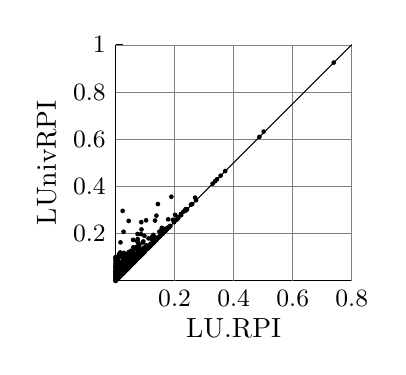
\begin{tikzpicture}

\draw (0,0) -- (3,0);
\node at (1.5,-0.6) {LU.RPI};
\node [anchor=north] at (0.75,0) {\small 0.2};
\draw (0.75,0) -- (0.75,0.1);
\draw [style=help lines] (0.75,0) -- (0.75,3);
\node [anchor=north] at (1.5,0) {\small 0.4};
\draw (1.5,0) -- (1.5,0.1);
\draw [style=help lines] (1.5,0) -- (1.5,3);
\node [anchor=north] at (2.25,0) {\small 0.6};
\draw (2.25,0) -- (2.25,0.1);
\draw [style=help lines] (2.25,0) -- (2.25,3);
\node [anchor=north] at (3,0) {\small 0.8};
\draw (3,0) -- (3,0.1);
\draw [style=help lines] (3,0) -- (3,3);
\draw (0,0) -- (0,3);
\node [rotate=90] at (-2.5em,1.5) {LUnivRPI};
\node [anchor=east] at (0,0.599) {\small 0.2};
\draw (0,0.599) -- (0.1,0.599);
\draw [style=help lines] (0,0.599) -- (3,0.599);
\node [anchor=east] at (0,1.198) {\small 0.4};
\draw (0,1.198) -- (0.1,1.198);
\draw [style=help lines] (0,1.198) -- (3,1.198);
\node [anchor=east] at (0,1.797) {\small 0.6};
\draw (0,1.797) -- (0.1,1.797);
\draw [style=help lines] (0,1.797) -- (3,1.797);
\node [anchor=east] at (0,2.396) {\small 0.8};
\draw (0,2.396) -- (0.1,2.396);
\draw [style=help lines] (0,2.396) -- (3,2.396);
\node [anchor=east] at (0,2.995) {\small 1};
\draw (0,2.995) -- (0.1,2.995);
\draw [style=help lines] (0,2.995) -- (3,2.995);
\foreach \pos in {
	(0.000000, 0.000000),
	(0.004367, 0.004367),
	(0.000000, 0.010490),
	(0.009009, 0.009009),
	(0.005300, 0.015901),
	(0.013333, 0.013333),
	(0.000000, 0.020408),
	(0.007344, 0.022032),
	(0.013363, 0.020045),
	(0.000000, 0.026882),
	(0.019405, 0.019405),
	(0.013550, 0.026197),
	(0.019874, 0.025552),
	(0.010545, 0.031634),
	(0.018545, 0.031636),
	(0.025974, 0.025974),
	(0.000000, 0.039063),
	(0.025373, 0.032836),
	(0.018394, 0.037707),
	(0.031185, 0.031185),
	(0.004545, 0.045455),
	(0.025199, 0.039059),
	(0.014706, 0.044118),
	(0.031370, 0.037975),
	(0.022222, 0.044444),
	(0.029126, 0.043689),
	(0.037514, 0.037514),
	(0.013756, 0.051586),
	(0.024965, 0.049931),
	(0.035319, 0.043629),
	(0.000000, 0.057143),
	(0.018544, 0.056083),
	(0.032504, 0.049358),
	(0.041806, 0.041806),
	(0.038687, 0.049238),
	(0.031774, 0.055605),
	(0.016529, 0.061983),
	(0.023281, 0.060209),
	(0.045596, 0.046526),
	(0.006696, 0.066964),
	(0.039003, 0.055255),
	(0.000000, 0.068571),
	(0.044633, 0.052604),
	(0.012821, 0.068376),
	(0.032098, 0.061848),
	(0.050346, 0.050346),
	(0.024150, 0.067084),
	(0.038633, 0.062407),
	(0.045249, 0.058824),
	(0.032609, 0.068182),
	(0.051980, 0.056436),
	(0.007692, 0.076923),
	(0.017266, 0.075540),
	(0.026026, 0.074074),
	(0.044056, 0.065035),
	(0.038710, 0.070968),
	(0.050669, 0.063336),
	(0.032518, 0.074326),
	(0.000000, 0.081571),
	(0.057884, 0.057884),
	(0.048237, 0.069573),
	(0.056680, 0.064777),
	(0.038541, 0.077081),
	(0.062169, 0.062169),
	(0.044843, 0.076233),
	(0.055670, 0.071134),
	(0.051040, 0.076560),
	(0.062092, 0.068627),
	(0.039669, 0.084298),
	(0.012371, 0.092784),
	(0.031250, 0.088542),
	(0.046997, 0.082245),
	(0.000000, 0.094737),
	(0.021583, 0.093525),
	(0.057252, 0.077290),
	(0.068311, 0.068311),
	(0.064439, 0.074463),
	(0.053834, 0.083197),
	(0.044355, 0.088710),
	(0.037480, 0.092140),
	(0.007732, 0.100515),
	(0.000000, 0.102273),
	(0.063299, 0.080563),
	(0.070661, 0.074380),
	(0.032653, 0.097959),
	(0.019531, 0.101562),
	(0.052678, 0.089552),
	(0.041763, 0.097448),
	(0.013216, 0.105727),
	(0.069543, 0.081133),
	(0.060287, 0.088995),
	(0.076194, 0.076730),
	(0.028754, 0.105431),
	(0.000000, 0.110656),
	(0.048387, 0.099620),
	(0.068465, 0.087137),
	(0.056354, 0.096133),
	(0.075997, 0.083597),
	(0.063315, 0.094398),
	(0.020814, 0.112217),
	(0.043307, 0.106299),
	(0.005894, 0.114931),
	(0.031250, 0.111111),
	(0.082120, 0.082120),
	(0.053088, 0.103467),
	(0.074447, 0.090543),
	(0.062016, 0.100775),
	(0.040036, 0.112100),
	(0.025424, 0.116949),
	(0.080873, 0.088575),
	(0.000000, 0.120000),
	(0.069740, 0.098109),
	(0.051241, 0.109315),
	(0.086692, 0.086692),
	(0.076923, 0.096154),
	(0.012903, 0.122581),
	(0.031447, 0.119497),
	(0.061141, 0.108016),
	(0.083228, 0.094578),
	(0.041152, 0.119342),
	(0.068666, 0.106551),
	(0.056897, 0.113793),
	(0.074353, 0.103448),
	(0.050562, 0.117978),
	(0.002568, 0.128425),
	(0.091082, 0.091082),
	(0.081818, 0.102273),
	(0.089029, 0.097122),
	(0.064000, 0.116000),
	(0.070423, 0.112676),
	(0.076867, 0.109810),
	(0.027815, 0.131126),
	(0.016667, 0.133333),
	(0.095588, 0.095588),
	(0.056133, 0.124740),
	(0.082873, 0.108919),
	(0.088710, 0.104839),
	(0.037736, 0.132075),
	(0.047771, 0.128981),
	(0.069638, 0.119777),
	(0.077381, 0.116071),
	(0.095112, 0.103038),
	(0.101449, 0.097826),
	(0.087800, 0.112463),
	(0.068581, 0.125733),
	(0.055147, 0.132353),
	(0.083937, 0.117150),
	(0.076110, 0.122622),
	(0.000000, 0.145374),
	(0.100313, 0.106583),
	(0.095785, 0.111111),
	(0.024974, 0.146722),
	(0.088995, 0.120574),
	(0.106322, 0.106322),
	(0.078750, 0.128250),
	(0.102094, 0.112565),
	(0.072331, 0.134328),
	(0.096642, 0.118421),
	(0.108247, 0.112113),
	(0.089313, 0.128244),
	(0.061100, 0.144603),
	(0.069124, 0.141014),
	(0.102981, 0.119241),
	(0.095553, 0.126202),
	(0.057508, 0.150160),
	(0.083333, 0.137821),
	(0.114044, 0.114044),
	(0.109091, 0.119580),
	(0.078303, 0.141925),
	(0.102439, 0.125854),
	(0.000000, 0.164234),
	(0.099321, 0.132428),
	(0.091537, 0.138169),
	(0.115963, 0.120258),
	(0.111603, 0.125775),
	(0.107034, 0.129969),
	(0.048649, 0.162162),
	(0.035176, 0.165829),
	(0.064815, 0.157407),
	(0.072041, 0.154374),
	(0.098131, 0.140187),
	(0.086411, 0.148449),
	(0.121919, 0.121919),
	(0.106017, 0.137536),
	(0.058099, 0.163732),
	(0.114645, 0.131379),
	(0.092923, 0.150154),
	(0.123322, 0.128356),
	(0.101266, 0.146835),
	(0.079937, 0.159875),
	(0.070968, 0.164516),
	(0.108216, 0.144289),
	(0.117455, 0.137031),
	(0.000000, 0.180516),
	(0.064549, 0.169057),
	(0.123364, 0.134579),
	(0.129405, 0.129405),
	(0.089457, 0.159744),
	(0.115279, 0.142726),
	(0.058172, 0.174515),
	(0.076807, 0.167169),
	(0.101485, 0.153465),
	(0.082797, 0.165593),
	(0.112957, 0.149502),
	(0.123203, 0.141684),
	(0.131300, 0.135279),
	(0.103752, 0.160522),
	(0.109464, 0.157355),
	(0.036036, 0.189189),
	(0.064994, 0.181300),
	(0.115243, 0.155701),
	(0.130321, 0.143354),
	(0.089503, 0.172376),
	(0.137931, 0.137931),
	(0.123377, 0.152597),
	(0.105882, 0.167647),
	(0.130977, 0.149688),
	(0.098811, 0.172919),
	(0.136153, 0.145436),
	(0.073171, 0.185976),
	(0.120000, 0.160000),
	(0.000000, 0.200000),
	(0.087097, 0.180645),
	(0.114343, 0.165496),
	(0.142857, 0.142857),
	(0.050251, 0.195980),
	(0.104690, 0.174204),
	(0.129114, 0.159494),
	(0.080153, 0.188931),
	(0.141579, 0.148902),
	(0.121896, 0.165914),
	(0.072581, 0.193548),
	(0.091037, 0.186309),
	(0.147541, 0.147541),
	(0.104558, 0.180965),
	(0.140461, 0.157233),
	(0.079439, 0.196262),
	(0.146341, 0.154044),
	(0.099338, 0.188742),
	(0.131918, 0.168309),
	(0.126923, 0.173077),
	(0.152098, 0.152098),
	(0.105606, 0.187744),
	(0.143609, 0.163715),
	(0.151007, 0.158557),
	(0.138462, 0.171041),
	(0.076043, 0.208504),
	(0.157022, 0.157022),
	(0.000000, 0.222222),
	(0.082695, 0.206738),
	(0.114607, 0.191011),
	(0.130035, 0.182969),
	(0.152968, 0.164384),
	(0.058496, 0.217270),
	(0.147368, 0.171053),
	(0.101983, 0.203966),
	(0.159151, 0.164456),
	(0.037696, 0.226178),
	(0.126667, 0.191667),
	(0.140244, 0.182927),
	(0.153696, 0.173152),
	(0.146341, 0.180775),
	(0.110400, 0.206400),
	(0.165517, 0.165517),
	(0.162562, 0.171429),
	(0.157895, 0.179825),
	(0.081720, 0.225806),
	(0.169811, 0.169811),
	(0.138500, 0.197857),
	(0.130796, 0.203460),
	(0.165000, 0.177500),
	(0.073952, 0.231717),
	(0.091640, 0.226688),
	(0.160305, 0.186478),
	(0.036855, 0.243243),
	(0.117383, 0.217447),
	(0.174832, 0.174832),
	(0.147241, 0.198888),
	(0.170616, 0.180095),
	(0.141768, 0.205793),
	(0.166768, 0.186927),
	(0.111570, 0.226240),
	(0.000000, 0.252632),
	(0.137405, 0.213740),
	(0.176471, 0.183007),
	(0.156904, 0.202406),
	(0.106401, 0.233564),
	(0.174194, 0.188710),
	(0.148897, 0.209559),
	(0.018979, 0.257569),
	(0.126246, 0.225914),
	(0.184265, 0.185645),
	(0.172748, 0.198404),
	(0.143089, 0.221138),
	(0.179919, 0.194070),
	(0.087549, 0.250973),
	(0.159218, 0.213687),
	(0.186090, 0.191729),
	(0.172708, 0.204691),
	(0.155620, 0.220461),
	(0.192913, 0.192913),
	(0.173021, 0.214076),
	(0.166667, 0.219807),
	(0.196144, 0.198659),
	(0.188247, 0.206175),
	(0.161448, 0.228963),
	(0.000000, 0.281250),
	(0.179543, 0.218716),
	(0.174515, 0.224377),
	(0.196721, 0.206557),
	(0.190733, 0.213362),
	(0.203103, 0.203103),
	(0.171912, 0.230255),
	(0.164122, 0.236641),
	(0.186441, 0.220339),
	(0.199434, 0.212164),
	(0.000000, 0.291262),
	(0.032258, 0.290323),
	(0.102857, 0.274286),
	(0.147082, 0.254475),
	(0.207242, 0.209385),
	(0.193746, 0.222298),
	(0.187500, 0.228659),
	(0.155405, 0.252252),
	(0.175127, 0.239502),
	(0.000000, 0.300000),
	(0.202222, 0.222222),
	(0.212085, 0.213270),
	(0.161815, 0.256849),
	(0.183414, 0.245157),
	(0.144695, 0.270096),
	(0.100000, 0.290000),
	(0.214651, 0.219761),
	(0.209607, 0.229258),
	(0.186158, 0.250597),
	(0.152406, 0.272727),
	(0.201705, 0.238636),
	(0.058906, 0.307153),
	(0.221352, 0.222331),
	(0.218373, 0.228163),
	(0.115481, 0.298745),
	(0.226619, 0.226619),
	(0.218613, 0.234416),
	(0.139535, 0.290698),
	(0.215548, 0.240283),
	(0.132813, 0.296875),
	(0.226929, 0.236006),
	(0.231984, 0.231984),
	(0.187879, 0.269697),
	(0.176471, 0.277311),
	(0.216190, 0.248766),
	(0.199367, 0.265823),
	(0.140318, 0.303087),
	(0.109261, 0.316857),
	(0.064516, 0.329032),
	(0.237251, 0.237251),
	(0.158654, 0.295673),
	(0.227538, 0.248541),
	(0.043668, 0.336245),
	(0.191411, 0.280982),
	(0.235075, 0.246269),
	(0.227891, 0.258503),
	(0.118705, 0.323741),
	(0.243958, 0.243958),
	(0.240810, 0.250938),
	(0.248040, 0.250178),
	(0.237617, 0.262165),
	(0.201622, 0.292005),
	(0.230769, 0.270243),
	(0.131542, 0.330976),
	(0.248189, 0.257278),
	(0.254325, 0.254325),
	(0.236659, 0.271462),
	(0.210291, 0.293065),
	(0.058824, 0.358289),
	(0.253898, 0.260579),
	(0.169231, 0.323077),
	(0.221591, 0.289773),
	(0.246938, 0.271926),
	(0.205319, 0.306520),
	(0.105263, 0.354067),
	(0.254672, 0.272290),
	(0.250319, 0.278416),
	(0.155709, 0.342561),
	(0.261307, 0.271357),
	(0.210913, 0.317943),
	(0.258845, 0.281588),
	(0.268408, 0.274660),
	(0.247633, 0.296431),
	(0.164948, 0.350515),
	(0.269118, 0.282353),
	(0.277142, 0.280612),
	(0.239244, 0.317943),
	(0.264770, 0.298770),
	(0.168717, 0.363796),
	(0.212286, 0.340591),
	(0.283951, 0.283951),
	(0.279141, 0.291411),
	(0.249370, 0.317380),
	(0.287571, 0.288790),
	(0.265165, 0.311958),
	(0.210402, 0.352246),
	(0.283113, 0.298013),
	(0.288703, 0.294979),
	(0.275902, 0.310827),
	(0.240711, 0.345719),
	(0.215617, 0.362023),
	(0.284424, 0.311512),
	(0.298747, 0.298747),
	(0.282723, 0.321990),
	(0.303598, 0.303598),
	(0.198748, 0.381847),
	(0.219101, 0.375000),
	(0.308964, 0.308964),
	(0.299220, 0.320808),
	(0.311100, 0.315789),
	(0.304147, 0.325872),
	(0.299177, 0.332113),
	(0.313433, 0.326866),
	(0.320900, 0.320900),
	(0.304718, 0.344037),
	(0.326425, 0.326425),
	(0.286082, 0.363402),
	(0.329558, 0.331823),
	(0.315517, 0.346552),
	(0.245758, 0.405500),
	(0.334153, 0.336481),
	(0.259375, 0.403125),
	(0.339950, 0.339950),
	(0.226212, 0.425494),
	(0.336909, 0.346372),
	(0.318277, 0.371849),
	(0.346776, 0.347547),
	(0.062593, 0.487332),
	(0.339768, 0.355212),
	(0.312461, 0.383260),
	(0.352941, 0.352941),
	(0.312599, 0.396989),
	(0.354227, 0.362974),
	(0.303797, 0.406872),
	(0.269164, 0.431185),
	(0.322008, 0.393822),
	(0.337748, 0.384106),
	(0.362745, 0.362745),
	(0.368852, 0.368852),
	(0.373610, 0.373610),
	(0.355536, 0.391869),
	(0.352518, 0.402878),
	(0.373989, 0.387863),
	(0.366838, 0.394823),
	(0.302178, 0.454628),
	(0.380041, 0.397149),
	(0.356890, 0.418728),
	(0.288312, 0.479221),
	(0.381215, 0.414365),
	(0.223118, 0.518817),
	(0.401936, 0.401936),
	(0.397554, 0.406728),
	(0.277014, 0.498035),
	(0.402672, 0.412214),
	(0.408727, 0.408727),
	(0.277710, 0.507917),
	(0.406977, 0.423256),
	(0.417994, 0.419088),
	(0.390733, 0.448967),
	(0.414600, 0.429483),
	(0.346939, 0.486395),
	(0.280665, 0.530146),
	(0.426829, 0.426829),
	(0.412541, 0.442244),
	(0.419624, 0.438413),
	(0.352941, 0.499160),
	(0.438213, 0.439599),
	(0.444500, 0.444500),
	(0.102273, 0.622159),
	(0.439739, 0.459283),
	(0.457012, 0.462020),
	(0.447280, 0.471457),
	(0.279534, 0.594010),
	(0.472072, 0.472072),
	(0.323544, 0.592405),
	(0.478431, 0.478431),
	(0.366848, 0.570652),
	(0.418803, 0.538462),
	(0.485581, 0.485581),
	(0.456221, 0.530876),
	(0.495146, 0.509709),
	(0.508130, 0.508130),
	(0.462236, 0.552870),
	(0.515304, 0.515304),
	(0.329557, 0.651724),
	(0.486435, 0.556467),
	(0.500000, 0.551282),
	(0.530574, 0.533396),
	(0.479458, 0.581758),
	(0.534354, 0.544858),
	(0.541339, 0.549213),
	(0.167102, 0.759791),
	(0.549662, 0.552555),
	(0.566875, 0.567790),
	(0.566994, 0.574067),
	(0.326656, 0.744222),
	(0.581419, 0.596404),
	(0.586279, 0.591913),
	(0.557185, 0.624633),
	(0.592893, 0.592893),
	(0.598803, 0.600378),
	(0.583914, 0.617694),
	(0.605854, 0.605854),
	(0.387597, 0.767442),
	(0.627142, 0.627142),
	(0.590070, 0.662635),
	(0.089888, 0.887640),
	(0.628999, 0.633153),
	(0.588167, 0.671694),
	(0.637417, 0.637417),
	(0.501528, 0.764732),
	(0.640533, 0.662722),
	(0.655066, 0.656275),
	(0.664245, 0.671352),
	(0.675813, 0.675813),
	(0.681072, 0.682819),
	(0.519183, 0.826939),
	(0.691057, 0.691057),
	(0.696561, 0.696870),
	(0.669130, 0.780000),
	(0.743390, 0.743390),
	(0.743363, 0.750603),
	(0.728400, 0.774335),
	(0.772600, 0.772600),
	(0.538050, 0.973996),
	(0.790795, 0.790795),
	(0.756032, 0.836461),
	(0.797386, 0.799020),
	(0.790571, 0.808437),
	(0.833239, 0.833239),
	(0.829088, 0.847749),
	(0.861519, 0.877792),
	(0.889159, 0.889507),
	(0.888000, 0.896000),
	(0.887715, 0.907530),
	(0.900283, 0.900283),
	(0.708972, 1.066740),
	(0.909224, 0.909224),
	(0.958415, 0.967221),
	(0.973150, 0.973150),
	(1.023024, 1.023024),
	(1.010802, 1.055671),
	(1.232750, 1.232750),
	(1.264940, 1.264940),
	(1.289613, 1.289613),
	(1.334389, 1.334389),
	(1.393080, 1.393080),
	(1.827128, 1.827128),
	(1.881198, 1.894112),
	(2.770800, 2.770800),
} \fill \pos circle(0.03);
\draw (0,0) -- (3, 3);
\end{tikzpicture}

  } \
  \subfloat[Compression ratio difference]{
    \centering
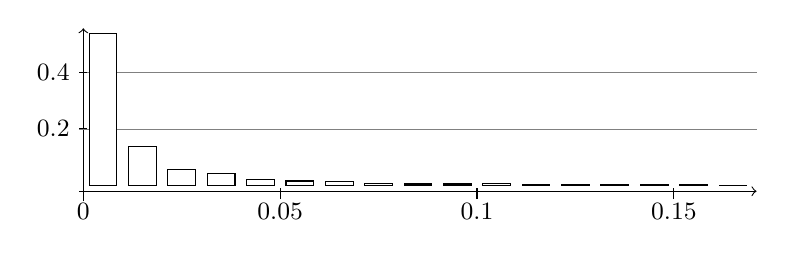
\begin{tikzpicture}
\draw[->] (-0.25,-0.2) -- (-0.25,2);
\draw [style=help lines] (-0.3,0.720894419908818) -- (8.3,0.720894419908818);
\node [anchor=east,fill=white] at (-0.3,0.720894419908818) {\small 0.2};
\draw (-0.3,0.720894419908818) -- (-0.2,0.720894419908818);
\draw [style=help lines] (-0.3,1.44178883981764) -- (8.3,1.44178883981764);
\node [anchor=east,fill=white] at (-0.3,1.44178883981764) {\small 0.4};
\draw (-0.3,1.44178883981764) -- (-0.2,1.44178883981764);
\draw[->] (-0.3,-0.07) -- (8.3,-0.07);
\node [anchor=north] at (-0.25, -0.1) {\small 0};
\draw (-0.25,-0.17) -- (-0.25,-0.03);
\node [anchor=north] at (2.25, -0.1) {\small 0.05};
\draw (2.25,-0.17) -- (2.25,-0.03);
\node [anchor=north] at (4.75, -0.1) {\small 0.1};
\draw (4.75,-0.17) -- (4.75,-0.03);
\node [anchor=north] at (7.25, -0.1) {\small 0.15};
\draw (7.25,-0.17) -- (7.25,-0.03);

\draw[fill=white] plot[ybar] coordinates {
	(6.000000, 0.011416)
	(6.500000, 0.009989)
	(7.500000, 0.011416)
	(3.000000, 0.047803)
	(5.500000, 0.017837)
	(5.000000, 0.024972)
	(8.000000, 0.002854)
	(1.500000, 0.151257)
	(4.500000, 0.021404)
	(3.500000, 0.028539)
	(0.500000, 0.492298)
	(0.000000, 1.927811)
	(4.000000, 0.022118)
	(2.500000, 0.059932)
	(1.000000, 0.209048)
	(2.000000, 0.077769)
	(7.000000, 0.010702)
};

\end{tikzpicture}
  } \
  \subfloat[Duration difference]{
    \centering
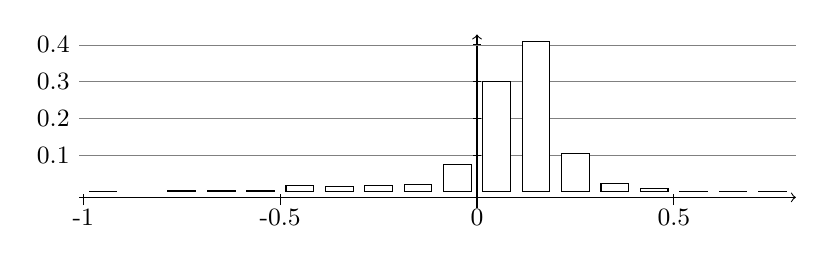
\begin{tikzpicture}
\draw[->] (-0.25,-0.2) -- (-0.25,2);
\draw [style=help lines] (-5.3,0.466521185853302) -- (3.8,0.466521185853302);
\node [anchor=east,fill=white] at (-5.3,0.466521185853302) {\small 0.1};
\draw (-0.3,0.466521185853302) -- (-0.2,0.466521185853302);
\draw [style=help lines] (-5.3,0.933042371706605) -- (3.8,0.933042371706605);
\node [anchor=east,fill=white] at (-5.3,0.933042371706605) {\small 0.2};
\draw (-0.3,0.933042371706605) -- (-0.2,0.933042371706605);
\draw [style=help lines] (-5.3,1.39956355755991) -- (3.8,1.39956355755991);
\node [anchor=east,fill=white] at (-5.3,1.39956355755991) {\small 0.3};
\draw (-0.3,1.39956355755991) -- (-0.2,1.39956355755991);
\draw [style=help lines] (-5.3,1.86608474341321) -- (3.8,1.86608474341321);
\node [anchor=east,fill=white] at (-5.3,1.86608474341321) {\small 0.4};
\draw (-0.3,1.86608474341321) -- (-0.2,1.86608474341321);
\draw[->] (-5.3,-0.07) -- (3.8,-0.07);
\node [anchor=north] at (-5.25, -0.1) {\small -1};
\draw (-5.25,-0.17) -- (-5.25,-0.03);
\node [anchor=north] at (-2.75, -0.1) {\small -0.5};
\draw (-2.75,-0.17) -- (-2.75,-0.03);
\node [anchor=north] at (-0.25, -0.1) {\small 0};
\draw (-0.25,-0.17) -- (-0.25,-0.03);
\node [anchor=north] at (2.25, -0.1) {\small 0.5};
\draw (2.25,-0.17) -- (2.25,-0.03);

\draw[fill=white] plot[ybar] coordinates {
	(1.000000, 0.485172)
	(-4.000000, 0.015710)
	(3.500000, 0.000924)
	(1.500000, 0.100731)
	(0.000000, 1.404689)
	(2.000000, 0.038814)
	(-3.500000, 0.017559)
	(0.500000, 1.906496)
	(-0.500000, 0.352096)
	(-3.000000, 0.019407)
	(3.000000, 0.006469)
	(-2.000000, 0.065614)
	(-1.000000, 0.095186)
	(2.500000, 0.004621)
	(-1.500000, 0.081324)
	(-5.000000, 0.000924)
	(-2.500000, 0.076703)
};

\end{tikzpicture}
  }
  \caption{Comparison between LU.RPI and LUnivRPI}
  \label{fig:LUnivRPI}
\end{figure}

\begin{figure}[!tbh]
  \centering
  \subfloat[Nodes compression]{
    \centering
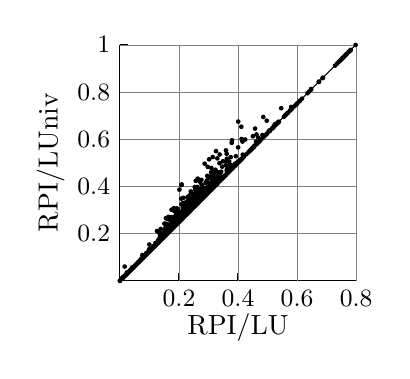
\begin{tikzpicture}

\draw (0,0) -- (3,0);
\node at (1.5,-0.6) {RPI/LU};
\node [anchor=north] at (0.75,0) {\small 0.2};
\draw (0.75,0) -- (0.75,0.1);
\draw [style=help lines] (0.75,0) -- (0.75,3);
\node [anchor=north] at (1.5,0) {\small 0.4};
\draw (1.5,0) -- (1.5,0.1);
\draw [style=help lines] (1.5,0) -- (1.5,3);
\node [anchor=north] at (2.25,0) {\small 0.6};
\draw (2.25,0) -- (2.25,0.1);
\draw [style=help lines] (2.25,0) -- (2.25,3);
\node [anchor=north] at (3,0) {\small 0.8};
\draw (3,0) -- (3,0.1);
\draw [style=help lines] (3,0) -- (3,3);
\draw (0,0) -- (0,3);
\node [rotate=90] at (-2.5em,1.5) {RPI/LUniv};
\node [anchor=east] at (0,0.599) {\small 0.2};
\draw (0,0.599) -- (0.1,0.599);
\draw [style=help lines] (0,0.599) -- (3,0.599);
\node [anchor=east] at (0,1.198) {\small 0.4};
\draw (0,1.198) -- (0.1,1.198);
\draw [style=help lines] (0,1.198) -- (3,1.198);
\node [anchor=east] at (0,1.797) {\small 0.6};
\draw (0,1.797) -- (0.1,1.797);
\draw [style=help lines] (0,1.797) -- (3,1.797);
\node [anchor=east] at (0,2.396) {\small 0.8};
\draw (0,2.396) -- (0.1,2.396);
\draw [style=help lines] (0,2.396) -- (3,2.396);
\node [anchor=east] at (0,2.995) {\small 1};
\draw (0,2.995) -- (0.1,2.995);
\draw [style=help lines] (0,2.995) -- (3,2.995);
\foreach \pos in {
	(0.000000, 0.000000),
	(0.022556, 0.022556),
	(0.028846, 0.028846),
	(0.034884, 0.034884),
	(0.034575, 0.044224),
	(0.039735, 0.039735),
	(0.047782, 0.047782),
	(0.055046, 0.055046),
	(0.063559, 0.063559),
	(0.068354, 0.068354),
	(0.072680, 0.072680),
	(0.077295, 0.077295),
	(0.083333, 0.083333),
	(0.088235, 0.088235),
	(0.092593, 0.092593),
	(0.090106, 0.106007),
	(0.099919, 0.099919),
	(0.104167, 0.104167),
	(0.110092, 0.110092),
	(0.114504, 0.114504),
	(0.122041, 0.122041),
	(0.128571, 0.128571),
	(0.060000, 0.180000),
	(0.134328, 0.134328),
	(0.139535, 0.139535),
	(0.146341, 0.146341),
	(0.151899, 0.151899),
	(0.156632, 0.156632),
	(0.162712, 0.162712),
	(0.155592, 0.170178),
	(0.168000, 0.168000),
	(0.172727, 0.172727),
	(0.177515, 0.177515),
	(0.182657, 0.182657),
	(0.190909, 0.190909),
	(0.195918, 0.195918),
	(0.204545, 0.204545),
	(0.209031, 0.210782),
	(0.214286, 0.214286),
	(0.223520, 0.223520),
	(0.230207, 0.230207),
	(0.234894, 0.234919),
	(0.239276, 0.239276),
	(0.243542, 0.243542),
	(0.248894, 0.248894),
	(0.255319, 0.255319),
	(0.260870, 0.260870),
	(0.265161, 0.265161),
	(0.269456, 0.269456),
	(0.273906, 0.273906),
	(0.273399, 0.280788),
	(0.279310, 0.279310),
	(0.283665, 0.283665),
	(0.288177, 0.288177),
	(0.292768, 0.292768),
	(0.298169, 0.298169),
	(0.302475, 0.302475),
	(0.293392, 0.314537),
	(0.285714, 0.326531),
	(0.306965, 0.306965),
	(0.311249, 0.311249),
	(0.307344, 0.320919),
	(0.315701, 0.315701),
	(0.320000, 0.320000),
	(0.324290, 0.324290),
	(0.328846, 0.328846),
	(0.333115, 0.333115),
	(0.337672, 0.337672),
	(0.334023, 0.351093),
	(0.342781, 0.342781),
	(0.347107, 0.347107),
	(0.351436, 0.351436),
	(0.356186, 0.356186),
	(0.360815, 0.360815),
	(0.365155, 0.365155),
	(0.369511, 0.369511),
	(0.373937, 0.373937),
	(0.367742, 0.387097),
	(0.378198, 0.378198),
	(0.382585, 0.382585),
	(0.376535, 0.388813),
	(0.371429, 0.400000),
	(0.386917, 0.386917),
	(0.393034, 0.393034),
	(0.397562, 0.397562),
	(0.401857, 0.401857),
	(0.406375, 0.406375),
	(0.410853, 0.410853),
	(0.415160, 0.415160),
	(0.374026, 0.459740),
	(0.419624, 0.419624),
	(0.423901, 0.423901),
	(0.428396, 0.428396),
	(0.424779, 0.438053),
	(0.432732, 0.432732),
	(0.437045, 0.437045),
	(0.441445, 0.441445),
	(0.445946, 0.445946),
	(0.450247, 0.450247),
	(0.455032, 0.455032),
	(0.453988, 0.463190),
	(0.459627, 0.459627),
	(0.464058, 0.464058),
	(0.452772, 0.480493),
	(0.468604, 0.468604),
	(0.472529, 0.473147),
	(0.469036, 0.478173),
	(0.477301, 0.477301),
	(0.481520, 0.481669),
	(0.485884, 0.485884),
	(0.490173, 0.490173),
	(0.484552, 0.498631),
	(0.494647, 0.494647),
	(0.498943, 0.498943),
	(0.486376, 0.514986),
	(0.503489, 0.503489),
	(0.507843, 0.507843),
	(0.512121, 0.512121),
	(0.505290, 0.524333),
	(0.516563, 0.516563),
	(0.520836, 0.520836),
	(0.522202, 0.527531),
	(0.516432, 0.533646),
	(0.504505, 0.547297),
	(0.528235, 0.528235),
	(0.522737, 0.542180),
	(0.532627, 0.532760),
	(0.531639, 0.539432),
	(0.537339, 0.537339),
	(0.542719, 0.542719),
	(0.543210, 0.549383),
	(0.508541, 0.583443),
	(0.549483, 0.549483),
	(0.554040, 0.554040),
	(0.544983, 0.564446),
	(0.471406, 0.631404),
	(0.531310, 0.582785),
	(0.558336, 0.558336),
	(0.488716, 0.622150),
	(0.557851, 0.566116),
	(0.563276, 0.563276),
	(0.557138, 0.574966),
	(0.529631, 0.602062),
	(0.567565, 0.567565),
	(0.501548, 0.631579),
	(0.572156, 0.572156),
	(0.567413, 0.578345),
	(0.576451, 0.576451),
	(0.563269, 0.593023),
	(0.513793, 0.636782),
	(0.573937, 0.585028),
	(0.580786, 0.581102),
	(0.567213, 0.603279),
	(0.585698, 0.585698),
	(0.574521, 0.599500),
	(0.583853, 0.591965),
	(0.591197, 0.591197),
	(0.518575, 0.657316),
	(0.587852, 0.597674),
	(0.578804, 0.611413),
	(0.596056, 0.596056),
	(0.600436, 0.600436),
	(0.599182, 0.606665),
	(0.605743, 0.605743),
	(0.579055, 0.635736),
	(0.610072, 0.610072),
	(0.607038, 0.615836),
	(0.614314, 0.614314),
	(0.576528, 0.655027),
	(0.618696, 0.618696),
	(0.609499, 0.630607),
	(0.615862, 0.624674),
	(0.623385, 0.623385),
	(0.604396, 0.645604),
	(0.579172, 0.671915),
	(0.619091, 0.635455),
	(0.627629, 0.627629),
	(0.632453, 0.632453),
	(0.615000, 0.650000),
	(0.604654, 0.662460),
	(0.633770, 0.638396),
	(0.611448, 0.660885),
	(0.584448, 0.689799),
	(0.606099, 0.670902),
	(0.629898, 0.648786),
	(0.639971, 0.639971),
	(0.636640, 0.645105),
	(0.644521, 0.644521),
	(0.640524, 0.649809),
	(0.617414, 0.675462),
	(0.635745, 0.658723),
	(0.624677, 0.671080),
	(0.648810, 0.648810),
	(0.564516, 0.725806),
	(0.641739, 0.660000),
	(0.636181, 0.669347),
	(0.651007, 0.655034),
	(0.603910, 0.699890),
	(0.649264, 0.662651),
	(0.657046, 0.657046),
	(0.611856, 0.701699),
	(0.589047, 0.722834),
	(0.650054, 0.669556),
	(0.657262, 0.663150),
	(0.645587, 0.676679),
	(0.663366, 0.663366),
	(0.631579, 0.696026),
	(0.614787, 0.711224),
	(0.660642, 0.671048),
	(0.667712, 0.667712),
	(0.657781, 0.679395),
	(0.655275, 0.686478),
	(0.664818, 0.677870),
	(0.672091, 0.672091),
	(0.636464, 0.707735),
	(0.670759, 0.680804),
	(0.677592, 0.677592),
	(0.657919, 0.700094),
	(0.671053, 0.687673),
	(0.679898, 0.683739),
	(0.666377, 0.702867),
	(0.680531, 0.690265),
	(0.686222, 0.686222),
	(0.661905, 0.714286),
	(0.676278, 0.701955),
	(0.656997, 0.720137),
	(0.690207, 0.690718),
	(0.686749, 0.699050),
	(0.674586, 0.711498),
	(0.693730, 0.695701),
	(0.666436, 0.722491),
	(0.686551, 0.706074),
	(0.672750, 0.719469),
	(0.585000, 0.795000),
	(0.699173, 0.699173),
	(0.601744, 0.784884),
	(0.691631, 0.710638),
	(0.697838, 0.705653),
	(0.703506, 0.703506),
	(0.640477, 0.764626),
	(0.705528, 0.709296),
	(0.691391, 0.723974),
	(0.702654, 0.715858),
	(0.642857, 0.772321),
	(0.711353, 0.711353),
	(0.612200, 0.799564),
	(0.679403, 0.744086),
	(0.689479, 0.735838),
	(0.709169, 0.720197),
	(0.703796, 0.726198),
	(0.715607, 0.715607),
	(0.703447, 0.732583),
	(0.715622, 0.722339),
	(0.710557, 0.727827),
	(0.615471, 0.810538),
	(0.721623, 0.721623),
	(0.719154, 0.727382),
	(0.709091, 0.737455),
	(0.725977, 0.725977),
	(0.653998, 0.793416),
	(0.721056, 0.734896),
	(0.730298, 0.730298),
	(0.711864, 0.750934),
	(0.707565, 0.755245),
	(0.718587, 0.749042),
	(0.731223, 0.736893),
	(0.727116, 0.742152),
	(0.656402, 0.807131),
	(0.737315, 0.737315),
	(0.733916, 0.743356),
	(0.679455, 0.794554),
	(0.723061, 0.755287),
	(0.691835, 0.786651),
	(0.719430, 0.762805),
	(0.741595, 0.742261),
	(0.740860, 0.750481),
	(0.746283, 0.746283),
	(0.721226, 0.775403),
	(0.734307, 0.763916),
	(0.742369, 0.756337),
	(0.750945, 0.750945),
	(0.736556, 0.770166),
	(0.751733, 0.758256),
	(0.723367, 0.786867),
	(0.745988, 0.766667),
	(0.757756, 0.757756),
	(0.752684, 0.764985),
	(0.716299, 0.801980),
	(0.752401, 0.771689),
	(0.759689, 0.764564),
	(0.729960, 0.795848),
	(0.765690, 0.765690),
	(0.760481, 0.771571),
	(0.755313, 0.782041),
	(0.723266, 0.811805),
	(0.769972, 0.769972),
	(0.705698, 0.829587),
	(0.765550, 0.775120),
	(0.743241, 0.801787),
	(0.739398, 0.806589),
	(0.761697, 0.786026),
	(0.756048, 0.792339),
	(0.774511, 0.774511),
	(0.753434, 0.798561),
	(0.771886, 0.781614),
	(0.763525, 0.793033),
	(0.778997, 0.778997),
	(0.715630, 0.840574),
	(0.737750, 0.822142),
	(0.748544, 0.812621),
	(0.727506, 0.833901),
	(0.783251, 0.783251),
	(0.777257, 0.791325),
	(0.762066, 0.807790),
	(0.749400, 0.821457),
	(0.774128, 0.798694),
	(0.785828, 0.788723),
	(0.655539, 0.901366),
	(0.782642, 0.797149),
	(0.775382, 0.805242),
	(0.791336, 0.791336),
	(0.766423, 0.817518),
	(0.789440, 0.797977),
	(0.686636, 0.889401),
	(0.795703, 0.795703),
	(0.725580, 0.860251),
	(0.776240, 0.816971),
	(0.759069, 0.834783),
	(0.788613, 0.807126),
	(0.765501, 0.829889),
	(0.750887, 0.845244),
	(0.745050, 0.851485),
	(0.800198, 0.800198),
	(0.797650, 0.807626),
	(0.804878, 0.804878),
	(0.795670, 0.817321),
	(0.780034, 0.832610),
	(0.801751, 0.813846),
	(0.793231, 0.823470),
	(0.788285, 0.828452),
	(0.807352, 0.810701),
	(0.775347, 0.841624),
	(0.685934, 0.921002),
	(0.800772, 0.823262),
	(0.797583, 0.828399),
	(0.813160, 0.813160),
	(0.773913, 0.851304),
	(0.743192, 0.879349),
	(0.760956, 0.864542),
	(0.810405, 0.819653),
	(0.794891, 0.836066),
	(0.817518, 0.817518),
	(0.814633, 0.825043),
	(0.796970, 0.843939),
	(0.810100, 0.831380),
	(0.823249, 0.823249),
	(0.718232, 0.917127),
	(0.815930, 0.832961),
	(0.796702, 0.852804),
	(0.822704, 0.830357),
	(0.730435, 0.914907),
	(0.828722, 0.828722),
	(0.818344, 0.842386),
	(0.824618, 0.836685),
	(0.809772, 0.854244),
	(0.830561, 0.834719),
	(0.816191, 0.849370),
	(0.836507, 0.836507),
	(0.825656, 0.847522),
	(0.800174, 0.872085),
	(0.813369, 0.861497),
	(0.834846, 0.844571),
	(0.840804, 0.840804),
	(0.792668, 0.891277),
	(0.839437, 0.849106),
	(0.829018, 0.861318),
	(0.845339, 0.845339),
	(0.835309, 0.857018),
	(0.843663, 0.853915),
	(0.849943, 0.849943),
	(0.831642, 0.870304),
	(0.842868, 0.861835),
	(0.817490, 0.889734),
	(0.854385, 0.854385),
	(0.830192, 0.881616),
	(0.836333, 0.875889),
	(0.858629, 0.858629),
	(0.810302, 0.904523),
	(0.849268, 0.869078),
	(0.854866, 0.865772),
	(0.844833, 0.879440),
	(0.863090, 0.863090),
	(0.857504, 0.871212),
	(0.852905, 0.876391),
	(0.798065, 0.926844),
	(0.866416, 0.868119),
	(0.861459, 0.875801),
	(0.808989, 0.926966),
	(0.871476, 0.871476),
	(0.856620, 0.889567),
	(0.865559, 0.880976),
	(0.850642, 0.899650),
	(0.875905, 0.875905),
	(0.872278, 0.884108),
	(0.880187, 0.880187),
	(0.860104, 0.899827),
	(0.852154, 0.907903),
	(0.780932, 0.969881),
	(0.870641, 0.895388),
	(0.876223, 0.889961),
	(0.832646, 0.932528),
	(0.884812, 0.884812),
	(0.853571, 0.917857),
	(0.883771, 0.891089),
	(0.879188, 0.895939),
	(0.819048, 0.952381),
	(0.889901, 0.889901),
	(0.828105, 0.948557),
	(0.867544, 0.915443),
	(0.890313, 0.896229),
	(0.881337, 0.908468),
	(0.896487, 0.896487),
	(0.892822, 0.902159),
	(0.799509, 0.986088),
	(0.888781, 0.907241),
	(0.877256, 0.918412),
	(0.867686, 0.930551),
	(0.900775, 0.900775),
	(0.901455, 0.906816),
	(0.897629, 0.912307),
	(0.873987, 0.935151),
	(0.907524, 0.907524),
	(0.855407, 0.958964),
	(0.904252, 0.914622),
	(0.894432, 0.926162),
	(0.902376, 0.920924),
	(0.910233, 0.913311),
	(0.868816, 0.953706),
	(0.827487, 0.991831),
	(0.900675, 0.926712),
	(0.880952, 0.946429),
	(0.915789, 0.915789),
	(0.844404, 0.984751),
	(0.911868, 0.922679),
	(0.859499, 0.974954),
	(0.920292, 0.920292),
	(0.778462, 1.043077),
	(0.907734, 0.936228),
	(0.917160, 0.927380),
	(0.901863, 0.943602),
	(0.924282, 0.925189),
	(0.886838, 0.963884),
	(0.867151, 0.982356),
	(0.908609, 0.945412),
	(0.902359, 0.951996),
	(0.929044, 0.929044),
	(0.917621, 0.943050),
	(0.926438, 0.935266),
	(0.851064, 1.005319),
	(0.908888, 0.954164),
	(0.933714, 0.933714),
	(0.917570, 0.950108),
	(0.886308, 0.980440),
	(0.929002, 0.941410),
	(0.904551, 0.967971),
	(0.915227, 0.958005),
	(0.805046, 1.052752),
	(0.870377, 1.000718),
	(0.938019, 0.938019),
	(0.927492, 0.948640),
	(0.917024, 0.964235),
	(0.936800, 0.946139),
	(0.942328, 0.942328),
	(0.913968, 0.970043),
	(0.935025, 0.953735),
	(0.910714, 0.977303),
	(0.923242, 0.967155),
	(0.876581, 1.011339),
	(0.946985, 0.946985),
	(0.884116, 1.008492),
	(0.894031, 1.003702),
	(0.946739, 0.954917),
	(0.942331, 0.959465),
	(0.953089, 0.953089),
	(0.921077, 0.985401),
	(0.943629, 0.966023),
	(0.951886, 0.959079),
	(0.912752, 0.997763),
	(0.958144, 0.958144),
	(0.956033, 0.964861),
	(0.944439, 0.979488),
	(0.962388, 0.962388),
	(0.858491, 1.056604),
	(0.912423, 1.012113),
	(0.954717, 0.975300),
	(0.959497, 0.970726),
	(0.966633, 0.966633),
	(0.860929, 1.062904),
	(0.940284, 0.995261),
	(0.971646, 0.971646),
	(0.963698, 0.980202),
	(0.969974, 0.978543),
	(0.943434, 1.006061),
	(0.975962, 0.975962),
	(0.955972, 0.996108),
	(0.755824, 1.156857),
	(0.902839, 1.046414),
	(0.957053, 1.003469),
	(0.981510, 0.981510),
	(0.921896, 1.039591),
	(0.978479, 0.990199),
	(0.986849, 0.986849),
	(0.976336, 0.997710),
	(0.951340, 1.025150),
	(0.985279, 0.992893),
	(0.969540, 1.008833),
	(0.884826, 1.084095),
	(0.911830, 1.064688),
	(0.992565, 0.992565),
	(0.941653, 1.042139),
	(0.980429, 1.008388),
	(0.929524, 1.058189),
	(0.967981, 1.024694),
	(0.995857, 0.997987),
	(0.907174, 1.079490),
	(0.960949, 1.033354),
	(0.939538, 1.054509),
	(0.977804, 1.019264),
	(0.948931, 1.047469),
	(0.990729, 1.011281),
	(1.001337, 1.001337),
	(0.995803, 1.007495),
	(0.977811, 1.026282),
	(1.006866, 1.006866),
	(0.989917, 1.025460),
	(0.994538, 1.021549),
	(1.004433, 1.014016),
	(0.924413, 1.087845),
	(0.962345, 1.055291),
	(1.011217, 1.011217),
	(1.002201, 1.022014),
	(0.983035, 1.043887),
	(1.009144, 1.018942),
	(1.014960, 1.017123),
	(0.925102, 1.101931),
	(1.006697, 1.029618),
	(1.020561, 1.020561),
	(0.781395, 1.213953),
	(0.900196, 1.133580),
	(1.008410, 1.039535),
	(1.025228, 1.025228),
	(0.784158, 1.223762),
	(1.023075, 1.032527),
	(1.030220, 1.030220),
	(0.985150, 1.074251),
	(0.980671, 1.080101),
	(1.023445, 1.039952),
	(1.031003, 1.036613),
	(1.037290, 1.037290),
	(1.026266, 1.051058),
	(0.984796, 1.090229),
	(1.041736, 1.041736),
	(1.021963, 1.065716),
	(0.984356, 1.102574),
	(1.046367, 1.046367),
	(1.014286, 1.078125),
	(1.038595, 1.059489),
	(0.999782, 1.096430),
	(1.031776, 1.068690),
	(1.045581, 1.055586),
	(1.051187, 1.051187),
	(0.962523, 1.138026),
	(1.047671, 1.062539),
	(1.056832, 1.056832),
	(0.977609, 1.135946),
	(1.055407, 1.065589),
	(1.060348, 1.061789),
	(1.050448, 1.073349),
	(0.955121, 1.162619),
	(1.065301, 1.065301),
	(1.040462, 1.090318),
	(0.969112, 1.154440),
	(1.017183, 1.117377),
	(1.070118, 1.070118),
	(1.040359, 1.100149),
	(1.062668, 1.078841),
	(1.056362, 1.092229),
	(1.070364, 1.080795),
	(1.075812, 1.075812),
	(1.026941, 1.122916),
	(0.950818, 1.189381),
	(0.967894, 1.176977),
	(1.037749, 1.115992),
	(1.066224, 1.089365),
	(1.053140, 1.103060),
	(1.080901, 1.080901),
	(1.055921, 1.108553),
	(1.077129, 1.088425),
	(1.085480, 1.085480),
	(1.034333, 1.134348),
	(1.076367, 1.094943),
	(1.085980, 1.092552),
	(0.980943, 1.191575),
	(1.014676, 1.163140),
	(1.092050, 1.092050),
	(1.087045, 1.099190),
	(1.085311, 1.107405),
	(1.096560, 1.096560),
	(1.101071, 1.101071),
	(1.086230, 1.120984),
	(1.100694, 1.107639),
	(1.096237, 1.119396),
	(1.108909, 1.108909),
	(1.097439, 1.125835),
	(1.113313, 1.113313),
	(1.108549, 1.124032),
	(1.082350, 1.149307),
	(1.045283, 1.184906),
	(1.105612, 1.129337),
	(1.099692, 1.135663),
	(1.119196, 1.119196),
	(1.123512, 1.123512),
	(1.056962, 1.186709),
	(0.963855, 1.269076),
	(1.120687, 1.134780),
	(1.128039, 1.128039),
	(1.129691, 1.135809),
	(1.036769, 1.222841),
	(1.136653, 1.136653),
	(1.117200, 1.166722),
	(1.100043, 1.183606),
	(1.130453, 1.154833),
	(1.142905, 1.142905),
	(1.014583, 1.258333),
	(1.144034, 1.150956),
	(1.139928, 1.156574),
	(1.150000, 1.150000),
	(1.130957, 1.173465),
	(0.988318, 1.296729),
	(1.120709, 1.185167),
	(1.154525, 1.154525),
	(1.159526, 1.159526),
	(1.130999, 1.187648),
	(1.155479, 1.167466),
	(1.148479, 1.177728),
	(1.034849, 1.281158),
	(1.145148, 1.187249),
	(1.167316, 1.167316),
	(1.088946, 1.243523),
	(1.159404, 1.178616),
	(1.143168, 1.198694),
	(1.174062, 1.174062),
	(1.166234, 1.183766),
	(1.171171, 1.179986),
	(1.098513, 1.250000),
	(1.159054, 1.194127),
	(1.164706, 1.191091),
	(1.181774, 1.181774),
	(1.172253, 1.195509),
	(1.178065, 1.190829),
	(1.187518, 1.187518),
	(1.129749, 1.244508),
	(1.103516, 1.271484),
	(1.192339, 1.192339),
	(1.170301, 1.214187),
	(1.186272, 1.207268),
	(1.197578, 1.197578),
	(1.194319, 1.203166),
	(1.197446, 1.212346),
	(1.207103, 1.207103),
	(1.183099, 1.238353),
	(1.212305, 1.212305),
	(1.190635, 1.234337),
	(1.217028, 1.217028),
	(1.190251, 1.245091),
	(1.125215, 1.309592),
	(1.202442, 1.240116),
	(1.172671, 1.273506),
	(1.224753, 1.224753),
	(1.109126, 1.331650),
	(1.201560, 1.252276),
	(1.210578, 1.244665),
	(1.229266, 1.229266),
	(1.144089, 1.310965),
	(1.233697, 1.233697),
	(1.231035, 1.242958),
	(1.144879, 1.324124),
	(1.238337, 1.238337),
	(1.244295, 1.244295),
	(1.237974, 1.252401),
	(1.198622, 1.298507),
	(1.239249, 1.275591),
	(1.262582, 1.262582),
	(1.189323, 1.338606),
	(1.268694, 1.268694),
	(1.254972, 1.287251),
	(1.157691, 1.376792),
	(1.275787, 1.275787),
	(1.241476, 1.323706),
	(1.282375, 1.287532),
	(1.115066, 1.446763),
	(1.181159, 1.394203),
	(1.292056, 1.292147),
	(1.280041, 1.311609),
	(1.076031, 1.487214),
	(1.298528, 1.298528),
	(1.211951, 1.383555),
	(1.222754, 1.376289),
	(1.303531, 1.303531),
	(1.161605, 1.431670),
	(1.304299, 1.315419),
	(1.310432, 1.310432),
	(1.251429, 1.374384),
	(1.313556, 1.317254),
	(1.213831, 1.409976),
	(1.261043, 1.372918),
	(1.273395, 1.367228),
	(1.322578, 1.322578),
	(1.329128, 1.329128),
	(1.286185, 1.385123),
	(1.337716, 1.337716),
	(1.342159, 1.342159),
	(1.348711, 1.348711),
	(1.132280, 1.541633),
	(1.358798, 1.362090),
	(1.366492, 1.366492),
	(1.299348, 1.449475),
	(1.356591, 1.398109),
	(1.379602, 1.379602),
	(1.264211, 1.493362),
	(1.359561, 1.416285),
	(1.177952, 1.571003),
	(1.389168, 1.389168),
	(1.396409, 1.397567),
	(1.391871, 1.413727),
	(1.236818, 1.554117),
	(1.345186, 1.465742),
	(1.380055, 1.433494),
	(1.404695, 1.416993),
	(1.366564, 1.455302),
	(1.412117, 1.412117),
	(1.307241, 1.516634),
	(1.410308, 1.425982),
	(1.420317, 1.420317),
	(1.398478, 1.455142),
	(1.344907, 1.514129),
	(1.397770, 1.471375),
	(1.435560, 1.435560),
	(1.440811, 1.440811),
	(1.422489, 1.464520),
	(1.266976, 1.603686),
	(1.362281, 1.525040),
	(1.220294, 1.646425),
	(1.387931, 1.514224),
	(1.450662, 1.457387),
	(1.357798, 1.549803),
	(1.458224, 1.458224),
	(1.462692, 1.462692),
	(1.468891, 1.468891),
	(1.458469, 1.481672),
	(1.478172, 1.478172),
	(1.478777, 1.495085),
	(1.355323, 1.612954),
	(1.406478, 1.570410),
	(1.498013, 1.498013),
	(1.503409, 1.505404),
	(1.497406, 1.513621),
	(1.346996, 1.654945),
	(1.509183, 1.509183),
	(1.523141, 1.523141),
	(1.472189, 1.581065),
	(1.528378, 1.528378),
	(1.527110, 1.535317),
	(1.538012, 1.538012),
	(1.544983, 1.544983),
	(1.556802, 1.556802),
	(1.573389, 1.573389),
	(1.560165, 1.601374),
	(1.419553, 1.751436),
	(1.501434, 1.693444),
	(1.606623, 1.606623),
	(1.423582, 1.783982),
	(1.632543, 1.632543),
	(1.644841, 1.644841),
	(1.653870, 1.653870),
	(1.556609, 1.767589),
	(1.665806, 1.665806),
	(1.670283, 1.670283),
	(1.544963, 1.800000),
	(1.683074, 1.683074),
	(1.693806, 1.693806),
	(1.590639, 1.793561),
	(1.701794, 1.701794),
	(1.706790, 1.706790),
	(1.707772, 1.715235),
	(1.735704, 1.735704),
	(1.744768, 1.744768),
	(1.728638, 1.766849),
	(1.755382, 1.756413),
	(1.541934, 1.955813),
	(1.687959, 1.834537),
	(1.766223, 1.766223),
	(1.773655, 1.773655),
	(1.502194, 2.021453),
	(1.785152, 1.785152),
	(1.779854, 1.790575),
	(1.755213, 1.818250),
	(1.734592, 1.857796),
	(1.810567, 1.810567),
	(1.716975, 1.932441),
	(1.810131, 1.849900),
	(1.834640, 1.834640),
	(1.855539, 1.855539),
	(1.868804, 1.868804),
	(1.890277, 1.901899),
	(1.897379, 1.897379),
	(1.904224, 1.904224),
	(1.905562, 1.910953),
	(1.932687, 1.932687),
	(1.938574, 1.938574),
	(1.946175, 1.948244),
	(1.865014, 2.032478),
	(1.820835, 2.080332),
	(1.955203, 1.955203),
	(1.964163, 1.968298),
	(1.966156, 1.986146),
	(1.978911, 1.980897),
	(1.987261, 1.993111),
	(1.996257, 1.997716),
	(2.004235, 2.004235),
	(2.011581, 2.016846),
	(2.019159, 2.019159),
	(2.082724, 2.082724),
	(2.096291, 2.096291),
	(2.107660, 2.110754),
	(2.048547, 2.191131),
	(2.127244, 2.127244),
	(2.135859, 2.135859),
	(2.162073, 2.162073),
	(2.170420, 2.172437),
	(2.186389, 2.186389),
	(2.174544, 2.206955),
	(2.215284, 2.215284),
	(2.234410, 2.234410),
	(2.248334, 2.248334),
	(2.252819, 2.252819),
	(2.281871, 2.281871),
	(2.286710, 2.286710),
	(2.312344, 2.312344),
	(2.382145, 2.382145),
	(2.400839, 2.400839),
	(2.427526, 2.427875),
	(2.428310, 2.435646),
	(2.523868, 2.523868),
	(2.529708, 2.529708),
	(2.573387, 2.573387),
	(2.578916, 2.578916),
	(2.732408, 2.732408),
	(2.757845, 2.757845),
	(2.777794, 2.777794),
	(2.794091, 2.794091),
	(2.807822, 2.807822),
	(2.819653, 2.819653),
	(2.825481, 2.825481),
	(2.830657, 2.830657),
	(2.844497, 2.844497),
	(2.858762, 2.858762),
	(2.870029, 2.870029),
	(2.879296, 2.879296),
	(2.903025, 2.903025),
	(2.916072, 2.916072),
	(2.925152, 2.925152),
	(2.931903, 2.931903),
	(2.993609, 2.993609),
} \fill \pos circle(0.03);
\draw (0,0) -- (3, 3);
\end{tikzpicture}

  } \qquad
  \subfloat[Unsat core compression]{
    \centering
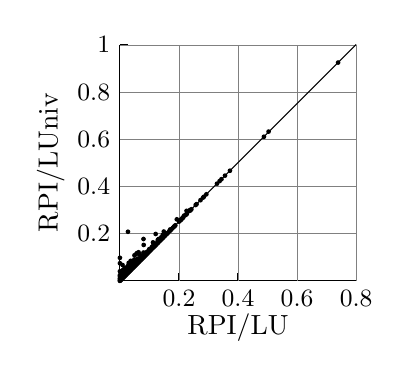
\begin{tikzpicture}

\draw (0,0) -- (3,0);
\node at (1.5,-0.6) {RPI/LU};
\node [anchor=north] at (0.75,0) {\small 0.2};
\draw (0.75,0) -- (0.75,0.1);
\draw [style=help lines] (0.75,0) -- (0.75,3);
\node [anchor=north] at (1.5,0) {\small 0.4};
\draw (1.5,0) -- (1.5,0.1);
\draw [style=help lines] (1.5,0) -- (1.5,3);
\node [anchor=north] at (2.25,0) {\small 0.6};
\draw (2.25,0) -- (2.25,0.1);
\draw [style=help lines] (2.25,0) -- (2.25,3);
\node [anchor=north] at (3,0) {\small 0.8};
\draw (3,0) -- (3,0.1);
\draw [style=help lines] (3,0) -- (3,3);
\draw (0,0) -- (0,3);
\node [rotate=90] at (-2.5em,1.5) {RPI/LUniv};
\node [anchor=east] at (0,0.599) {\small 0.2};
\draw (0,0.599) -- (0.1,0.599);
\draw [style=help lines] (0,0.599) -- (3,0.599);
\node [anchor=east] at (0,1.198) {\small 0.4};
\draw (0,1.198) -- (0.1,1.198);
\draw [style=help lines] (0,1.198) -- (3,1.198);
\node [anchor=east] at (0,1.797) {\small 0.6};
\draw (0,1.797) -- (0.1,1.797);
\draw [style=help lines] (0,1.797) -- (3,1.797);
\node [anchor=east] at (0,2.396) {\small 0.8};
\draw (0,2.396) -- (0.1,2.396);
\draw [style=help lines] (0,2.396) -- (3,2.396);
\node [anchor=east] at (0,2.995) {\small 1};
\draw (0,2.995) -- (0.1,2.995);
\draw [style=help lines] (0,2.995) -- (3,2.995);
\foreach \pos in {
	(0.000000, 0.000000),
	(0.004367, 0.004367),
	(0.008831, 0.008831),
	(0.007353, 0.014706),
	(0.013181, 0.013181),
	(0.000000, 0.020690),
	(0.017481, 0.017481),
	(0.011628, 0.023256),
	(0.021765, 0.021765),
	(0.000000, 0.031746),
	(0.018251, 0.027376),
	(0.026028, 0.026028),
	(0.022624, 0.031674),
	(0.018987, 0.037975),
	(0.030332, 0.030332),
	(0.014706, 0.044118),
	(0.026892, 0.038845),
	(0.034682, 0.034682),
	(0.025210, 0.045378),
	(0.032609, 0.043478),
	(0.038249, 0.039524),
	(0.000000, 0.057143),
	(0.029745, 0.050992),
	(0.043126, 0.043126),
	(0.039280, 0.047872),
	(0.047368, 0.047368),
	(0.039003, 0.055255),
	(0.032895, 0.059211),
	(0.000000, 0.070312),
	(0.046089, 0.054469),
	(0.051619, 0.051619),
	(0.033520, 0.067039),
	(0.042105, 0.063158),
	(0.007692, 0.076923),
	(0.051163, 0.058140),
	(0.057075, 0.057075),
	(0.041216, 0.069942),
	(0.027190, 0.081571),
	(0.061318, 0.061318),
	(0.050139, 0.071031),
	(0.057793, 0.068301),
	(0.044118, 0.080882),
	(0.065563, 0.065563),
	(0.061061, 0.074074),
	(0.055118, 0.078740),
	(0.069936, 0.069936),
	(0.064624, 0.081857),
	(0.040609, 0.096447),
	(0.074194, 0.074194),
	(0.057292, 0.088542),
	(0.073370, 0.081522),
	(0.068966, 0.086207),
	(0.078624, 0.078624),
	(0.045455, 0.102273),
	(0.020814, 0.112217),
	(0.066667, 0.093333),
	(0.078125, 0.085938),
	(0.083697, 0.083697),
	(0.000000, 0.120000),
	(0.079137, 0.093525),
	(0.046632, 0.113990),
	(0.087948, 0.087948),
	(0.061475, 0.110656),
	(0.032258, 0.122581),
	(0.078929, 0.100775),
	(0.072687, 0.105727),
	(0.089489, 0.093750),
	(0.085938, 0.101562),
	(0.095290, 0.095290),
	(0.092375, 0.101173),
	(0.033333, 0.133333),
	(0.052326, 0.127907),
	(0.061856, 0.123711),
	(0.087640, 0.107865),
	(0.075843, 0.117978),
	(0.099644, 0.099644),
	(0.094284, 0.109315),
	(0.074844, 0.124740),
	(0.103890, 0.103890),
	(0.066038, 0.132075),
	(0.084615, 0.123077),
	(0.097393, 0.115101),
	(0.103448, 0.111111),
	(0.109164, 0.109164),
	(0.107713, 0.115691),
	(0.099174, 0.123967),
	(0.113456, 0.113456),
	(0.092704, 0.131330),
	(0.110526, 0.121053),
	(0.104592, 0.127551),
	(0.117754, 0.117754),
	(0.064815, 0.157407),
	(0.117073, 0.124390),
	(0.107303, 0.134128),
	(0.059459, 0.162162),
	(0.123000, 0.123000),
	(0.113662, 0.134328),
	(0.121339, 0.129707),
	(0.127434, 0.127434),
	(0.104188, 0.150153),
	(0.115587, 0.141856),
	(0.126004, 0.133674),
	(0.079646, 0.165929),
	(0.131707, 0.131707),
	(0.085843, 0.167169),
	(0.121519, 0.146835),
	(0.126984, 0.142857),
	(0.135981, 0.135981),
	(0.121704, 0.154564),
	(0.132464, 0.146011),
	(0.140288, 0.140288),
	(0.033333, 0.200000),
	(0.144563, 0.144563),
	(0.135135, 0.155405),
	(0.148902, 0.148902),
	(0.130653, 0.165829),
	(0.102832, 0.187779),
	(0.150000, 0.155556),
	(0.134003, 0.174204),
	(0.156087, 0.156087),
	(0.000000, 0.222222),
	(0.117117, 0.189189),
	(0.153169, 0.163732),
	(0.133409, 0.181300),
	(0.160485, 0.160485),
	(0.131429, 0.188571),
	(0.140391, 0.182969),
	(0.155172, 0.171088),
	(0.164782, 0.164782),
	(0.114731, 0.203966),
	(0.163587, 0.171699),
	(0.169385, 0.169385),
	(0.162406, 0.180451),
	(0.121479, 0.211268),
	(0.173648, 0.173648),
	(0.168639, 0.183432),
	(0.178170, 0.178170),
	(0.111570, 0.226240),
	(0.160804, 0.195980),
	(0.166667, 0.191667),
	(0.174481, 0.190504),
	(0.182825, 0.182825),
	(0.187500, 0.187500),
	(0.185484, 0.193548),
	(0.144695, 0.226688),
	(0.191872, 0.191872),
	(0.176615, 0.208504),
	(0.190000, 0.200000),
	(0.185501, 0.204691),
	(0.196292, 0.196292),
	(0.201174, 0.201174),
	(0.196721, 0.206557),
	(0.190733, 0.213362),
	(0.136842, 0.252632),
	(0.185879, 0.220461),
	(0.205882, 0.205882),
	(0.199434, 0.212164),
	(0.000000, 0.291262),
	(0.193746, 0.222298),
	(0.164426, 0.245088),
	(0.210471, 0.210471),
	(0.204878, 0.221138),
	(0.214884, 0.214884),
	(0.216590, 0.221198),
	(0.186158, 0.250597),
	(0.222656, 0.222656),
	(0.219643, 0.230357),
	(0.227273, 0.227273),
	(0.218424, 0.237996),
	(0.211957, 0.244565),
	(0.183280, 0.270096),
	(0.226929, 0.236006),
	(0.231522, 0.231522),
	(0.236559, 0.236559),
	(0.230997, 0.248766),
	(0.240854, 0.240854),
	(0.238683, 0.246914),
	(0.246080, 0.246080),
	(0.245495, 0.252252),
	(0.251685, 0.251685),
	(0.237342, 0.265823),
	(0.222086, 0.280982),
	(0.232620, 0.272727),
	(0.255764, 0.258981),
	(0.261868, 0.261868),
	(0.184615, 0.323077),
	(0.246094, 0.281250),
	(0.252874, 0.278416),
	(0.266949, 0.266949),
	(0.271357, 0.271357),
	(0.275910, 0.275910),
	(0.269318, 0.289773),
	(0.280335, 0.280335),
	(0.209897, 0.342599),
	(0.279141, 0.291411),
	(0.285121, 0.286989),
	(0.265165, 0.311958),
	(0.290323, 0.290323),
	(0.283113, 0.298013),
	(0.216495, 0.350515),
	(0.258993, 0.323741),
	(0.294873, 0.294873),
	(0.248908, 0.336245),
	(0.299163, 0.299163),
	(0.289872, 0.310827),
	(0.303598, 0.303598),
	(0.236912, 0.362023),
	(0.297794, 0.316176),
	(0.303665, 0.314136),
	(0.308964, 0.308964),
	(0.314465, 0.314465),
	(0.309760, 0.330976),
	(0.320890, 0.320890),
	(0.319236, 0.327422),
	(0.325581, 0.325581),
	(0.299465, 0.358289),
	(0.331823, 0.331823),
	(0.336685, 0.336685),
	(0.332180, 0.342561),
	(0.342924, 0.342924),
	(0.348214, 0.348214),
	(0.337434, 0.363796),
	(0.352941, 0.352941),
	(0.360562, 0.360562),
	(0.368852, 0.368852),
	(0.370787, 0.375000),
	(0.363436, 0.383260),
	(0.377953, 0.377953),
	(0.373989, 0.387863),
	(0.384106, 0.384106),
	(0.377606, 0.393822),
	(0.302178, 0.454628),
	(0.374101, 0.402878),
	(0.383281, 0.397476),
	(0.393908, 0.393908),
	(0.393212, 0.405500),
	(0.399654, 0.399654),
	(0.401447, 0.406872),
	(0.411398, 0.411398),
	(0.418728, 0.418728),
	(0.407666, 0.431185),
	(0.420108, 0.425494),
	(0.426641, 0.426641),
	(0.425532, 0.432624),
	(0.419624, 0.438413),
	(0.299376, 0.530146),
	(0.434407, 0.434407),
	(0.426425, 0.448967),
	(0.439227, 0.439227),
	(0.443760, 0.443760),
	(0.102273, 0.622159),
	(0.449070, 0.449070),
	(0.453360, 0.453360),
	(0.420268, 0.487332),
	(0.459283, 0.459283),
	(0.447280, 0.471457),
	(0.472072, 0.472072),
	(0.478431, 0.478431),
	(0.485581, 0.485581),
	(0.480354, 0.498035),
	(0.490909, 0.490909),
	(0.481183, 0.518817),
	(0.508130, 0.508130),
	(0.492166, 0.530876),
	(0.513398, 0.513398),
	(0.518045, 0.518045),
	(0.454243, 0.594010),
	(0.533793, 0.533793),
	(0.538462, 0.538462),
	(0.525680, 0.552870),
	(0.541582, 0.544625),
	(0.548293, 0.548293),
	(0.553151, 0.553151),
	(0.544782, 0.581758),
	(0.558424, 0.570652),
	(0.567790, 0.567790),
	(0.574790, 0.574790),
	(0.571139, 0.592405),
	(0.581419, 0.596404),
	(0.589391, 0.589391),
	(0.557185, 0.624633),
	(0.595190, 0.595190),
	(0.601953, 0.601953),
	(0.609326, 0.609326),
	(0.626341, 0.626341),
	(0.631907, 0.633153),
	(0.640449, 0.640449),
	(0.645040, 0.645040),
	(0.638424, 0.651724),
	(0.656678, 0.656678),
	(0.671694, 0.671694),
	(0.684916, 0.684916),
	(0.691057, 0.691057),
	(0.697179, 0.697179),
	(0.703569, 0.703569),
	(0.750603, 0.750603),
	(0.722609, 0.780000),
	(0.760803, 0.764732),
	(0.767442, 0.767442),
	(0.772600, 0.772600),
	(0.777616, 0.777616),
	(0.790795, 0.790795),
	(0.797386, 0.799020),
	(0.804314, 0.804314),
	(0.814429, 0.826939),
	(0.833239, 0.833239),
	(0.844504, 0.844504),
	(0.850415, 0.850415),
	(0.846442, 0.887640),
	(0.861519, 0.877792),
	(0.889159, 0.889507),
	(0.888000, 0.896000),
	(0.900283, 0.900283),
	(0.907530, 0.907530),
	(0.962120, 0.962120),
	(0.973150, 0.973150),
	(1.023024, 1.023024),
	(1.055671, 1.055671),
	(1.066922, 1.066922),
	(1.097921, 1.097921),
	(1.232750, 1.232750),
	(1.265604, 1.265604),
	(1.289613, 1.289613),
	(1.334842, 1.334842),
	(1.397232, 1.397232),
	(1.828723, 1.828723),
	(1.887913, 1.894112),
	(2.770800, 2.770800),
} \fill \pos circle(0.03);
\draw (0,0) -- (3, 3);
\end{tikzpicture}

  } \
  \subfloat[Nodes compression difference]{
    \centering
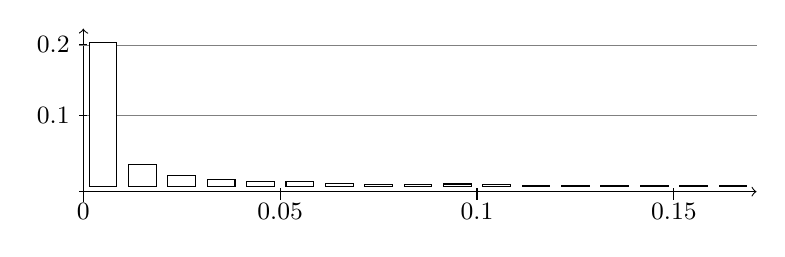
\begin{tikzpicture}
\draw[->] (-0.25,-0.2) -- (-0.25,2);
\draw [style=help lines] (-0.3,0.896638354122678) -- (8.3,0.896638354122678);
\node [anchor=east,fill=white] at (-0.3,0.896638354122678) {\small 0.1};
\draw (-0.3,0.896638354122678) -- (-0.2,0.896638354122678);
\draw [style=help lines] (-0.3,1.79327670824536) -- (8.3,1.79327670824536);
\node [anchor=east,fill=white] at (-0.3,1.79327670824536) {\small 0.2};
\draw (-0.3,1.79327670824536) -- (-0.2,1.79327670824536);
\draw[->] (-0.3,-0.07) -- (8.3,-0.07);
\node [anchor=north] at (-0.25, -0.1) {\small 0};
\draw (-0.25,-0.17) -- (-0.25,-0.03);
\node [anchor=north] at (2.25, -0.1) {\small 0.05};
\draw (2.25,-0.17) -- (2.25,-0.03);
\node [anchor=north] at (4.75, -0.1) {\small 0.1};
\draw (4.75,-0.17) -- (4.75,-0.03);
\node [anchor=north] at (7.25, -0.1) {\small 0.15};
\draw (7.25,-0.17) -- (7.25,-0.03);

\draw[fill=white] plot[ybar] coordinates {
	(4.500000, 0.026615)
	(3.500000, 0.017743)
	(0.500000, 0.278571)
	(6.000000, 0.010646)
	(0.000000, 1.820472)
	(6.500000, 0.007097)
	(4.000000, 0.023066)
	(7.500000, 0.007097)
	(3.000000, 0.031938)
	(5.500000, 0.010646)
	(5.000000, 0.017743)
	(8.000000, 0.007097)
	(2.500000, 0.053230)
	(1.000000, 0.133075)
	(2.000000, 0.055005)
	(7.000000, 0.001774)
	(1.500000, 0.079845)
};

\end{tikzpicture}
  } \
  \subfloat[Duration difference]{
    \centering
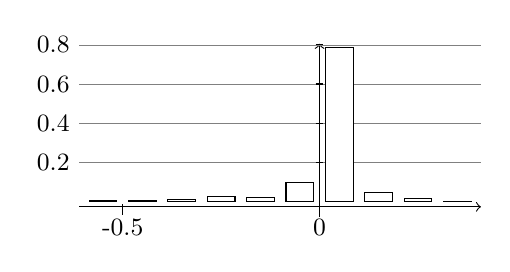
\begin{tikzpicture}
\draw[->] (-0.25,-0.2) -- (-0.25,2);
\draw [style=help lines] (-3.3,0.496543752673843) -- (1.8,0.496543752673843);
\node [anchor=east,fill=white] at (-3.3,0.496543752673843) {\small 0.2};
\draw (-0.3,0.496543752673843) -- (-0.2,0.496543752673843);
\draw [style=help lines] (-3.3,0.993087505347686) -- (1.8,0.993087505347686);
\node [anchor=east,fill=white] at (-3.3,0.993087505347686) {\small 0.4};
\draw (-0.3,0.993087505347686) -- (-0.2,0.993087505347686);
\draw [style=help lines] (-3.3,1.48963125802153) -- (1.8,1.48963125802153);
\node [anchor=east,fill=white] at (-3.3,1.48963125802153) {\small 0.6};
\draw (-0.3,1.48963125802153) -- (-0.2,1.48963125802153);
\draw [style=help lines] (-3.3,1.98617501069537) -- (1.8,1.98617501069537);
\node [anchor=east,fill=white] at (-3.3,1.98617501069537) {\small 0.8};
\draw (-0.3,1.98617501069537) -- (-0.2,1.98617501069537);
\draw[->] (-3.3,-0.07) -- (1.8,-0.07);
\node [anchor=north] at (-2.75, -0.1) {\small -0.5};
\draw (-2.75,-0.17) -- (-2.75,-0.03);
\node [anchor=north] at (-0.25, -0.1) {\small 0};
\draw (-0.25,-0.17) -- (-0.25,-0.03);

\draw[fill=white] plot[ybar] coordinates {
	(1.000000, 0.031963)
	(0.500000, 0.116543)
	(1.500000, 0.002459)
	(-0.500000, 0.234561)
	(-3.000000, 0.006884)
	(0.000000, 1.950246)
	(-2.000000, 0.022620)
	(-1.000000, 0.049174)
	(-1.500000, 0.062943)
	(-2.500000, 0.009343)
};

\end{tikzpicture}
  }
  \caption{Comparison between the LU and LUniv combinations}
\end{figure}


\section{Conclusions}

\bibliographystyle{splncs}
\bibliography{../biblio}

\end{document}
